\documentclass[11pt,oneside,a4paper,titlepage,onecolumn]{book}

\usepackage[utf8]{inputenc}
\usepackage{textcomp}
\usepackage[official]{eurosym}
\usepackage[polish]{babel}
\usepackage{amsthm}
\usepackage{graphicx}
\usepackage[T1]{fontenc}
\usepackage{scrextend}
\usepackage{hyperref}
\usepackage{xcolor}
\usepackage{enumitem}
% \usepackage{nameref}
% \usepackage{showlabels}
% \usepackage{titlesec}
\usepackage{geometry}
\geometry{a4paper, portrait, margin=2cm}
\graphicspath{ {./fig/} }
\usepackage{listings}

\newenvironment{enumreq}
{ \begin{enumerate}[topsep=0pt,itemsep=-1ex,partopsep=1ex,parsep=1ex] }
{ \end{enumerate}                  } 

\newcommand{\inzmaintitlePL}{Viua VM w akcji}

\setcounter{secnumdepth}{4}

%% Author and title
% \author{Marek Marecki \and Gr.52c \and Krzysztof Franek}
\author{Zespół: Marek Marecki i Krzysztof Franek\\Promotor: dr hab. Marek A. Bednarczyk, prof. PJWSTK}
\title{%
    \inzmaintitlePL \\
    \large
    Implementacja języka wysokiego poziomu i \\
    prostej aplikacji\\
    ~\\
    Viua VM in action.\\
    Implementation of a high-level programming language and\\ a simple application}

\begin{document}

\lstset{basicstyle=\ttfamily,
columns=fixed,
escapeinside={\%*}{*)},
inputencoding=utf8,
extendedchars=true}

\maketitle

\tableofcontents
% \listoftables
\listoffigures

Praca została złożona za pomocą systemu \LaTeX.

\newpage

\chapter{Wprowadzenie}

We wprowadzeniu chcielibyśmy poruszyć ogólne tematy związane z naszą pracą, oraz przedstawić Czytelnikowi
spójny wstęp zapewniający solidne podstawy do dalszej lektury. Zakładamy, że Czytelnik ma doświadczenie z
językami programowania i umie biegle posługiwać się co najmniej jednym ''\emph{mainstreamowym}'' językiem, np.
C++, Java, czy Python.

Wprowadzenie jest dla nas miejscem, w którym przedstawimy problemy dręczące popularne obecnie języki
programowania oraz powiemy skąd się te problemy biorą i dlaczego w miarę postępu technologii są one coraz
trudniejsze do zignorowania.

Po krótce przedstawiona zostanie również maszyna wirtualna Viua, która jest platformą, na której nasza praca
się opiera.

\section{Układ pracy inżynierskiej}

W rozdziale \ref{jezyk_viuact_i_jego_kompilator}.~\nameref{jezyk_viuact_i_jego_kompilator} (na stronie
\pageref{jezyk_viuact_i_jego_kompilator}) przedstawiamy język Viuact oraz jego implementację - kompilator.
Są to narzędzia wykorzystywane do stworzenia aplikacji użytkowej przedstawionej w rozdziale
\ref{program_viuachat}.~\nameref{program_viuachat} (na stronie \pageref{program_viuachat}).

Wkład własny członków zespołu przedstawiony jest w rozdziale \ref{wklad_wlasny_czlonkow_zespolu} na stronie
\pageref{wklad_wlasny_czlonkow_zespolu}.

W rozdziale \ref{slownik_pojec}.~\nameref{slownik_pojec} na stronie \pageref{slownik_pojec} prezentujemy listę
pojęć i terminów używanych w pracy, które mogą wymagać doprecyzowania lub definicji. Dla wygody Czytelnika są
one umieszczone w jednym miejscu, oraz podzielone na sekcje związane z językiem i kompilatorem
(rozdział~\ref{slownik_pojec_jezyka}) i związane z chatem (rozdział~\ref{slownik_pojec_chatu}).

\section{Przedstawienie problemu}

Tytułem pracy jest ,,\inzmaintitlePL''. Problemem, który poruszamy jest sprawdzenie czy Viua VM w stanie
,,zastanym'' (tj. w takim w jakim znajdowała się jej implementacja na początku prac nad projektem
inżynierskim) umożliwia pisanie niezawodnego, wysoce współbieżnego, nietrywialnego oprogramowania.

W naszej pracy prezentujemy język programowania, który z założenia ma pozwalać na tworzenie oprogramowania
niezawodnego i wykorzystującego potencjał współbieżności w stopniu wyższym niż powszechnie używane,
,,mainstreamowe'' języki programowania.

Aby udowodnić, że w wytworzonym języku możliwe jest tworzenie nietrywialnego oprogramowania prezenetujemy
aplikację użytkową -- czat -- napisany w tym języku. Czat umożliwi komunikację (zorganizowaną kanałach) wielu
użytkownikom naraz. Wybór rodzaju aplikacji (czat) jest warunkowany tym, że oprogramowanie komunikacyjne
powinno charakteryzować się tymi cechami, które chcemy uzyskać:

\begin{enumerate}
    \item niezawodnością -- jeśli jedno połączenie ulegnie awarii to pozostałe powinny działać dalej
    \item izolacją procesów -- każde połączenie powinno być izolowane od wszystkich innych
    \item współbieżnością -- wiele połączeń musi być obsługiwanych w tym samym czasie
\end{enumerate}

\subsection{Ogląd sytuacji}

Współczesny \emph{hardware} zmierza coraz bardziej w stronę współbieżności oraz przetwarzania równoległego.
Firma AMD w roku 2018 wprowadziła na rynek konsumencki procesory wielordzeniowe z serii
Threadripper\footnote{https://www.amd.com/en/products/ryzen-threadripper} prezentujące nawet 32 rdzenie logiczne.

Współczesny \emph{software} stoi w miejscu. Poza oprogramowaniem specjalistycznym (np.
Blender\footnote{https://www.blender.org/}) mało który program jest w stanie wykorzystać więcej niż kilka wątków.
Współbieżności szuka się nieco ''na siłę''; np. przeglądarki internetowe uruchamiają współbieżnie obsługę
wielu kart.

Mainstreamowe języki w większości korzystają z wątków (np. Java, C++) lub są stricte jednowątkowe i
niedostosowane do przetwarzania współbieżnego i równoległego (np. Python).

Dla takich języków tworzone są biblioteki ułatwiające wykorzystanie mechanizmów systemu operacyjnego
(np.~wieloprocesowość dla języka Python) lub cała infrastruktura umożliwiająca rozproszenie pracy,
np.~sewery pracy (np. Gearman, Celery) czy kolejki wiadomości (np. RabbitMQ, ZeroMQ).
To wszystko są jednak jedynie ''łatki'' mające za zadanie dodać do istniejących języków mechanizmy, z którymi
pierwotnie nie były one projektowane. Istnieje dla takiego działania angielski termin bardzo dobrze oddający
jego postać: \emph{retrofitting}.

Istnieją środowiska i języki zaprojektowane od zera z myślą o współbieżności i przetwarzaniu równoległym, a
nawet rozproszonym.
Najbardziej znanym przykładem takiego środowiska jest BEAM -- maszyna wirtualna
języka Erlang\footnote{http://www.erlang.org/}. To środowisko wraz z językiem jest z powodzeniem
wykorzystywane w sprzęcie telekomunikacyjnym firmy Ericsson, oraz do tworzenia aplikacji użytkowych, których
działanie obejmuje niemal z definicji działanie rozproszone i współbieżne, na przykład w serwerach
komunikatora Discord\footnote{https://discordapp.com/}.

\section{Cel}

Ta praca inżynierska motywowana jest chęcią stworzenia bazy programistycznej (środowiska uruchomieniowego i
języka programowania) umożliwiającej programistom pisanie oprogramowania od początku uwzględniającego
przetwarzanie współbieżne na pierwszym miejscu, oraz charakteryzującego się wysokim poziomem niezawodności i
stabliności działania.

Osiągniemy to dzięki zbudowaniu języka wyposażonego w łatwo dostępne konstrukcje umożliwiające wprowadzenie
współbieżności do programu, oraz uruchamianiu programów wynikowych w środowisku zdolnym do rozłożenia pracy na
całość dostępnych zasobów sprzętowych.

\subsection{Problemy i ryzyko}

Postawienie współbieżności na pierwszym miejscu powoduje, że problemy związane z pisaniem poprawnych programów
są bardziej liczne niż w innych (niewspółbieżnych) językach -- oprócz zapewnienia poprawności pojedynczego
procesu, programista musi zadbać o poprawność interakcji między procesami, oraz o stabilność działania
oprogramowania w momencie awarii któregoś z procesów składowych programu.

Zminimalizujemy ryzyko płynące z wprowadzenia współbieżności do warsztatu programistów udostępniając im
mechanizmy umożliwiające opanowanie awarii, propagowanie informacji o błędach, oraz izolację poszczególnych
procesów składowych.

\chapter{Strategia prowadzenia prac}

W tym rozdziale opisujemy metodologię prac nad poszczególnymi częściami projektu. Każda z nich była rozwijana
innym sposobem z dużych rozbieżności specyfiki konkretnych problemu -- zupełnie inaczej pracuje się nad
semi-formalną specyfikacją języka programowania niż nad aplikacją użytkową, więc podjęliśmy decyzję o
rozdzieleniu tych części i poprowadzeniu ich jako osobne, mniejsze projekty wewnątrz pracy inżynierskiej.

\section{Język ViuAct}

% Specyfikacja. Analiza wymagań. Formalizm. Kaskada.

Tworzenie specyfikacji języka odbywa się w modelu kaskadowo-prototypowym i przeplata się z implementacją
prototypu kompilatora.

\subsection{Określenie wymagań}

Przed rozpoczęciem specyfikowania poszczególnych konstrukcji językowych należało podjąć decyzję co w języku
powinno się znaleźć, a co nie powinno zostać włączone do specyfikacji.

\subsection{Specyfikacja konkretnej konstrukcji języka}

Każda konstrukcja językowa jest najpierw projektowana, następnie dokumentowana i omawiana (żeby wychwycić
pewne oczywiste błędy ,,grube'' na wczesnym etapie prac). Potem proces specyfikacji zostaje zawieszony do
momentu wytworzenia w kompilatorze prototypu danej konstrukcji, lub odrzucenia jej jako niewykonalnej w
zakładanym czasie lub zakresie funkcjonalności.

Wynik prac prototypowych (sukces bądź porażka) decyduje o tym czy prace specyfikacyjne są prowadzone dalej.
Jeśli konstrukcja jest możliwa do zaimplementowania jej specyfikacja jest formalizowana oraz przygotowana dla
niej zostaje dokumentacja (obejmująca m.in. przykłady użycia).

\section{Kompilator języka ViuAct}

Issue tracking, open-source. Prototypowanie. Iteracja.
Prace przeplatają się z pracami nad specyfikacją celem walidacji co jest możliwe.

\subsection{Testowanie}

Zestaw prostych programów testowych. Test sprawdza czy program się kompiluje i czy po uruchomieniu daje
spodziewane wyniki.

\section{Program ViuaChat}

Mini-SCRUM.

\subsection{Testowanie}

Jak wygląda testowanie czatu.

\chapter{Dokumentacja prac}

\section{Specyfikacja języka ViuAct}

Tworzenie formalnej specyfikacji języka ViuAct było, paradoksalnie, procesem mało sformalizowanym. Polegało
na określeniu głównych założeń języka (opisanych w rozdziale
\ref{specyfikacja_jezyka_viuact_model_programowania}
\nameref{specyfikacja_jezyka_viuact_model_programowania}).

\section{Implementacja kompilatora}

Issue tracking. Zapis issue, daty rozpoczęcia i zakończenia, branche z Git. Trochę słowno-muzycznego opisu co
się działo podczas prac.

\section{Implementacja ViuaChat}

Opis prac nad implementacją ViuaChat.

\chapter{Język ViuAct i jego kompilator -- formalności}

W tym rozdziale prezentujemy wszelkie ''formalności'' związane z pierwszą częścią naszej pracy, czyli
dokumenty takie jak DZW\footnote{Dokument Założeń Wstępnych} czy SWS\footnote{Spis Wymagań Systemowych}.
Opis projektu języka i jego implementacji prezentujemy w rozdziale \nameref{jezyk_viuact_i_jego_kompilator} na
stronie~\pageref{jezyk_viuact_i_jego_kompilator}.

\section{Wprowadzenie}

\subsection{Cel dokumentu}
Celem dokumentu jest zdefiniowanie wymagań dla czatu ViuaChat na podstawie analizy otoczenia aplikacji oraz analizy potrzeb projektu w stosunku do niej.

\subsection{Zakres dokumentu}
Niniejszy dokument jest produktem pierwszego etapu procesu wytwórczego czatu ViuaChat, na który składają się:
\begin{itemize}
    \item analiza otoczenia, wraz z z klientami;
    \item wskazanie kontekstu biznesowego systemu;
    \item określenie udziałowców;
	\item wyszczególnienie i uporządkowanie zasad biznesowych, jakie zostały założone w stosunku do aplikacji;
	\item opracowanie historyjek na podstawie ustalonych zasad biznesowych.
\end{itemize}

\textbf{Uwaga:} Niniejszy dokument nie dotyczy języka ViuAct ani jego kompilatora.

\subsection{Dokumenty powiązane}
\begin{itemize}
	\item Szkic funkcjonalności ViuaChat - pierwszy zarys zasad biznesowych, ujęty w formie prostego konspektu;
	\item Specyfikacja wymagań biznesowych i \textit{user stories} - starsza wersja dokumentu SWS, nieujmująca otoczenia i kontekstu aplikacji.
\end{itemize}

\subsection{Odbiorcy}
Dokument został skierowany przede wszystkim dla członków zespołu, aby ułatwić im współpracę - w szczególności wówczas, gdy funkcjonalności czatu mogą pociągać za sobą modyfikację zestawu bibliotek ViuaVM bądź struktury składni projektowanego języka ViuAct.

Kolejną grupą adresatów niniejszego dokumentu są pracownicy uczelni, odpowiedzialni za nadzór nad prawidłowym ukształtowaniem i przebiegiem projektu. Wśród nich, szczególną rolę odgrywa JE Dziekan ZWI, prof. Marek Bednarczyk, będący opiekunem projektu.

\section{Czat w kontekście}

\subsection{Kontekst biznesowy}

Niniejszy czat stanowi część szerszego kontekstu, jakim jest potrzeba zademonstrowania działania języka ViuAct oraz całego środowiska wytwórczego powiązanego z maszyną wirtualną ViuaVM.

\begin{figure}[h]
	\centering
	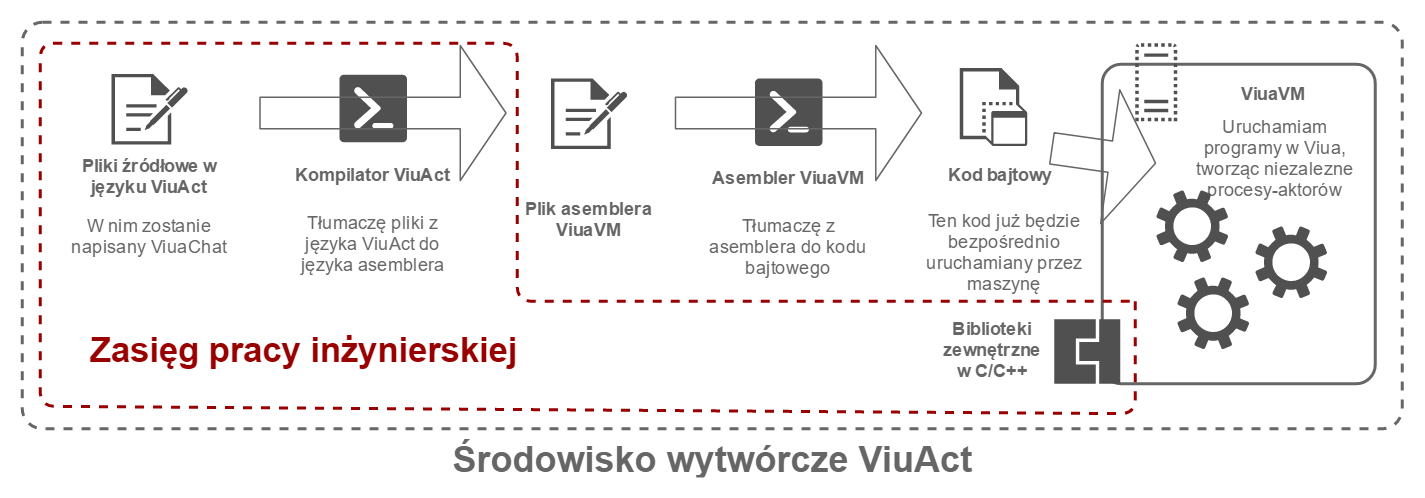
\includegraphics[width=\textwidth]{chat/fig/viuavm-env}
	\caption{Ilustracja środowiska wytwórczego wraz zasięgiem, którym są objęte prace przewidziane projektem inżynierskim}
\end{figure}

Cel demonstracyjny jest pierwszym i najważniejszym, jaki przyświeca konstrukcji czatu. Ponadto, sam proces wytwórczy pozwoli
przetestować wydajność całego środowiska w jego praktycznym wymiarze. Tym samym, możliwe będzie poprawienie konstrukcji kompilatora 
lub zastosowanych konstrukcji językowych ViuAct, podnoszących jego użyteczność.

Wszelcy odbiorcy dla aplikacji czatu zostaną, podobnie jak sama aplikacja, skonstruowani na cele demonstracyjne. Nie powinni oni
odbiegać od modelowych odbiorców podobnych komunikatorów, tak, aby potencjalny, poczatkujący użytkownik środowiska ViuaVM mógł
zrozumieć intencje stojące za rozwiązaniami zastosowanymi w ViuaChat oraz przenieść je do swoich pierwszych programów, opracowanych
w tym środowisku.

\subsection{Udziałowcy}

Poniżej wyszczególniono udziałowców, mających wpływ na rozwój czatu.

\begin{tabular}{ | l | l | }
  
	\hline
	\multicolumn{2}{ | l | }{\textbf{Karta udziałowca}}  \\
  
	\hline
    \parbox[t]{3cm}{
    	\textbf{Identyfikator}
    } & UN-01 \\  
    
    \hline
    \parbox[t]{3cm}{
    	\textbf{Nazwa}
    } & ViuaVM \\  
    
    \hline
    \parbox[t]{3cm}{
    	\textbf{Opis}
    } & \parbox[t]{12cm}{
    	Maszyna wirtualna, oparta o przechowywanie danych w rejestrach zamiast \textit{płaskich} tablic pamięci. Stanowi ona 
    	platformę, na której musi zostać uruchomiony serwer czatu. Ponieważ jej największym atutem jest zorientowanie na kod
    	wykonywany współbieżnie, sam serwer czatu powinien tę cechę wykorzystywać w maksymalnym stopniu. 
    	} \\ 
    
    \hline
    \parbox[t]{3cm}{
    	\textbf{Typ}
    } & Nieożywiony, bezpośredni \\  
    
    \hline
    \parbox[t]{3cm}{
    	\textbf{Punkt widzenia}
    } & \parbox[t]{12cm}{
    	ViuaVM jest absolutnie nieodzownym elementem projektu, a serwer czatu stanowi przede wszystkim dowód jej użyteczności.
    	O ile jądro maszyny nie ma być poddawane już żadnym zmianom i być wykorzystane takie, jakie było na inicjalnym etapie
    	pracy inżynierskiej, o tyle dopuszcza się poszerzanie jej funkcjonalności o dodatkowe biblioteki zewnętrzne.
    	} \\ 
    
    \hline
    \parbox[t]{3cm}{
    	\textbf{Ograniczenia}
    } & \parbox[t]{12cm}{
    	Maszyna wirtualna, jakkolwiek stanowi istotny czynnik dla decyzji w zakresie architektury czy konstrukcji oprogramowania,
    	nie powinna mieć wpływu na wymagania stricte biznesowe, jest bowiem jedynie środowiskiem do uruchamiania współbieżnych
    	programów, \textit{przezroczystym} dla końcowego użytkownika czy zleceniodawcy zrealizowanego oprogramowania.
    	} \\ 
    
    \hline
    \parbox[t]{3cm}{
    	\textbf{Wymagania}
    } & \colorbox{yellow}{...} \\ 
  
    \hline
\end{tabular}

\vspace{2em} 

\begin{tabular}{ | l | l | }

	\hline
	\multicolumn{2}{ | l | }{\textbf{Karta udziałowca}}  \\
  
	\hline
    \parbox[t]{3cm}{
    	\textbf{Identyfikator}
    } & UO-01 \\  
    
    \hline
    \parbox[t]{3cm}{
    	\textbf{Nazwa}
    } & Opiekun pracy inżynierskiej \\ 
    
    \hline
    \parbox[t]{3cm}{
    	\textbf{Opis}
    } & \parbox[t]{12cm}{
    	Pracownik uczelni, wyznaczony do opieki nad całym projektem inżynierskim - nadzorowania jego postępów, wskazywania problemów
    	oraz sugerowania decyzji podwyższających walor pracy oraz szanse na jej skuteczne obronienie. Ma również zasadniczy wpływ na 
    	decyzję o dopuszczeniu pracy do recenzji.
    } \\ 
    
    \hline
    \parbox[t]{3cm}{
    	\textbf{Typ}
    } & Ożywiony, bezpośredni \\  
    
    \hline
    \parbox[t]{3cm}{
    	\textbf{Punkt widzenia}
    } & \parbox[t]{12cm}{
    	Opiekun pracy patrzy na czat przede wszystkim przez pryzmat jego użyteczności jako efektownego przykładu implementacji modelu
    	aktora w praktycznym, programistycznym ujęciu. Stąd, jego uwaga skupia się przede wszystkim na konstrukcjach językowych,
    	strukturach oraz rozwiązaniach od strony kodu źródłowego. Czat stanowi jedynie pretekst do przeniesienia teoretycznych, akademickich
    	rozważań na praktyczny grunt. 
    	} \\ 
    
    \hline
    \parbox[t]{3cm}{
    	\textbf{Ograniczenia}
    } & \parbox[t]{12cm}{
    	Opiekun pracy, pomimo bycia jej nadzorcą i posiadania istotnych uprawnień decyzyjnych w stosunku do jej dalszego rozwoju, 
    	nie ma możliwości bieżącego śledzenia prac oraz
    	podejmowania decyzji w przypadku konkretnych problemów. Powinien zachować dystans, pozwalający na samodzielną realizację projektu
    	przez zespół. Stąd, jego faktyczny udział ogranicza się do udzielania porad w przypadku strategicznych kierunków, w jakich
    	będzie podążała grupa, a także doraźnego recenzowania ograniczonej puli zagadnień, wyłapanych w trakcie wspólnych spotkań.
    	} \\ 
    
    \hline
    \parbox[t]{3cm}{
    	\textbf{Wymagania}
    } & \colorbox{yellow}{...} \\ 
  
    \hline
\end{tabular}

\vspace{2em} 

\begin{tabular}{ | l | l | }

	\hline
	\multicolumn{2}{ | l | }{\textbf{Karta udziałowca}}  \\
  
	\hline
    \parbox[t]{3cm}{
    	\textbf{Identyfikator}
    } & UO-02 \\  
    
    \hline
    \parbox[t]{3cm}{
    	\textbf{Nazwa}
    } & \parbox[t]{12cm}{
    Członek zespołu ds. ViuAct
    } \\ 
    
    \hline
    \parbox[t]{3cm}{
    	\textbf{Opis}
    } & \parbox[t]{12cm}{
    	Student i członek zespołu, skupiający się w pierwszej kolejności nad rozwojem języka programowania ViuAct, jego kompilatora oraz
    	ewentualnego rozbudowania maszyny ViuaVM o kolejne, zewnętrzne biblioteki.
    } \\ 
    
    \hline
    \parbox[t]{3cm}{
    	\textbf{Typ}
    } & Ożywiony, bezpośredni \\  
    
    \hline
    \parbox[t]{3cm}{
    	\textbf{Punkt widzenia}
    } & \parbox[t]{12cm}{
    	Przede wszystkim, postrzega czat jako produkt, realizowany na końcowej platformie. Stąd, musi brać udział w formułowaniu
    	wymagań związanych z ViuaVM oraz językiem ViuAct. Jego zadaniem jest doprowadzenia do zaprojektowania czatu w sposób, 
    	który ukaże możliwości ViuAct jako solidnego, kompletnego rozwiązania. Przy tym, musi trzymać rękę na pulsie i reagować,
    	gdyby pojawiały się przeszkody w zaprogramowaniu czatu, wynikające z niedoskonałości środowiska wytwórczego.
    	
    	Podczas współudziału w definiowaniu wymagań, istotny jest dla niego zakres pracy, wiążący się z 
    	urzeczywistnianiem poszczególnych, proponowanych wymagań. Zbyt rozbudowany czat może opóźnić prace nad całym projektem,
    	a w efekcie - zniweczyć trud włożony w rozwój języka programowania i dedykowanego mu kompilatora.
    	} \\ 
    
    \hline
    \parbox[t]{3cm}{
    	\textbf{Ograniczenia}
    } & \parbox[t]{12cm}{
    	Jego udział w pracach nad czatem jest z gruntu nieograniczony. Jednakże, decydując się na podział odpowiedzialności 
    	podyktowany zespołowym charakterem projektu oraz własnymi ograniczeniami czasowymi, zrezygnował z decydowania o biznesowej 
    	części wymagań, faktycznie pozostając w roli konsultanta.
    	
    	} \\ 
    
    \hline
    \parbox[t]{3cm}{
    	\textbf{Wymagania}
    } & \colorbox{yellow}{...} \\ 
  
    \hline
\end{tabular}

\vspace{2em} 

\begin{tabular}{ | l | l | }

	\hline
	\multicolumn{2}{ | l | }{\textbf{Karta udziałowca}}  \\
  
	\hline
    \parbox[t]{3cm}{
    	\textbf{Identyfikator}
    } & UO-03 \\  
    
    \hline
    \parbox[t]{3cm}{
    	\textbf{Nazwa}
    } & \parbox[t]{12cm}{
    Członek zespołu ds. Czatu
    } \\ 
    
    \hline
    \parbox[t]{3cm}{
    	\textbf{Opis}
    } & \parbox[t]{12cm}{
    	Student i członek zespołu, odpowiedzialny za prace nad czatem
    } \\ 
    
    \hline
    \parbox[t]{3cm}{
    	\textbf{Typ}
    } & Ożywiony, bezpośredni \\  
    
    \hline
    \parbox[t]{3cm}{
    	\textbf{Punkt widzenia}
    } & \parbox[t]{12cm}{
    	Czat stanowi dla niego, obok dokumentacji, najistotniejszą część przedsięwzięcia. Musi z jednej strony nauczyć się poruszać
    	w nowym, dynamicznie zmieniającym się środowisku programistycznym, a z drugiej strony - zrealizować przy jego użyciu serwer
    	czatu, który pokaże jego możliwości i zastosowania innym nowicjuszom.
    	
    	Podczas współudziału w definiowaniu wymagań, istotny jest dla niego zakres końcowych funkcjonalności czatu. Nie może być zbyt 
    	wąski. Z drugiej strony, konstrukcja programu powinna pozostać prosta i przejrzysta. Przykładowy kod nie powinien odstraszać
    	potencjalnego programisty, dla którego cała koncepcja ViuaVM oraz modelu aktorów może wydawać się na pierwszy rzut oka nieco egzotyczna.
    	} \\ 
    
    \hline
    \parbox[t]{3cm}{
    	\textbf{Ograniczenia}
    } & \parbox[t]{12cm}{
    	Nie ma w zasadzie organizacyjnych czy kompetencyjnych ograniczeń dla formułowania wymagań. Nie oznacza to jednak, że może
    	definiować wymagań w oderwaniu od pozostałych udziałowców (ich role i punkty widzenia opisano wcześniej).
    	} \\ 
    
    \hline
    \parbox[t]{3cm}{
    	\textbf{Wymagania}
    } & \colorbox{yellow}{...} \\ 
  
    \hline
\end{tabular}

\subsection{Charakterystyka użytkowników}

Na etapie analizy kontekstu, w którym ma zostać zaprojektowany i zrealizowany czat, zadecydowano o zaprojektowaniu następujących,
modelowych użytkowników docelowego oprogramowania:

\begin{enumerate}

	\item \textbf{Użytkownik tymczasowy.} Typ użytkownika, którego konto jest tworzone podczas połączenia z serwerem czatu oraz 
		niszczone po jego zakończeniu. Podczas łączenia z czatem, nie będzie musiał się autoryzować przy użyciu hasła, a deklarować
		tylko unikalną nazwę, nie powtarzającą się z nazwą innego użytkownika, posiadającego konto na danym serwerze czatu. Ten typ
		konta jest przeznaczony dla osób, zainteresowanych dołączeniem do dyskusji na czacie bez dodatkowych zobowiązań.
		
	\item \textbf{Użytkownik stały.} Typ użytkownika, którego konto jest utrzymywane przez serwer pomiędzy połączeniami do czatu. W
		zamierzeniu, adresatami takiego rozwiązania mają być stali bywalcy serwera, którzy chcą mieć zarezerwowaną określoną nazwę
		dla siebie i uniknąć ewentualnego podszywania się. Stąd każdorazowo, przed rozpoczęciem sesji połączenia z serwerem, muszą się
		dodatkowo autoryzować przy użyciu hasła. Równocześnie, ich nazwa jest zarezerwowana wyłącznie do jego użytku oraz niedostępna
		dla użytkowników tymczasowych.
		
	\item \textbf{Administrator.} To użytkownik stały, który jest dodatkowo wyróżniony i posiada uprawienia do szeroko pojętego 
		zarządzania serwerem (w tym - pozostałymi użytkownikami). Nie wyróżnia się wśród administratorów żadnych dodatkowych, szczególnych
		ról (np. superadministrator, właściciel).
		
\end{enumerate}

Poza wspomnianymi różnicami, wszyscy użytkownicy po rozpoczęciu sesji połączenia mają prawo do dołączania do pokojów oraz wysyłania sobie
nawzajem wiadomości prywatnych. Łącznie, pula użytkowników przebywających na serwerze czatu w jednym momencie nie powinna przekraczać 320,
zaś w jednym pokoju - nie więcej niż 32. W związku z tym można przyjąć, że czat jest przeznaczony dla niewielkich społeczności, np.
szkolnych, uczelnianych czy hobbystycznych.

\subsection{Istniejąca infrastruktura}

\begin{itemize}
	\item \textbf{Komputer A}
	\begin{itemize}
		\item komputer przenośny z procesorem Intel Core i5 oraz systemem operacyjnym Windows 10
		\item XAMPP 7.2.7, obejmujący serwer Apache 2.4 oraz interpreter języka PHP w wersji 7.2.7.
	\end{itemize}
	
	\item \textbf{Komputer B}
	\begin{itemize}
		\item komputer przenośny, na którym zainstalowano system operacyjny Linux Mint 19 ,,Tara''
		\item GNU Compiler Collection 8.2
		\item wirtualna maszyna Viua VM w wersji 0.9.0
		\item \textit{należy doinstalować serwer Nginx, odpowiedzialny za wysłanie frontendu do
		użytkownika łączącego się z czatem oraz za handshake Websocketu}
	\end{itemize}
	
	\item \textit{\textbf{Do uzupełnienia}
	\begin{itemize}
		\item Kolejne urządzenie końcowe (trzecie), dzięki któremu będzie można symulować połączenie kolejnej
		osoby do usługi czatu
	\end{itemize}}

\end{itemize}

\section{Zasady biznesowe}

Zidentyfikowane zasady pogrupowano w 3 kategorie, biorąc pod uwagę podstawowe bloki funkcjonalności. Przydzielenie
do kategorii jest sygnalizowanie literą alfabetu, będącą prefiksem identyfikatora danej zasady. Dokonano
również priorytetyzacji zasad biznesowych według klasycznej skali ,,MoSCoW":

\begin{itemize}
	\item \textbf{,,M''} (z ang. \textit{must}) - zasady, których spełnienie jest niezbędne dla realizacji systemu
	\item \textbf{,,S''} (z ang. \textit{should}) - są to zasady o wysokim priorytecie, które powinny;
	zostać spełnione, o ile tylko jest to możliwe;
	\item \textbf{,,C''} (z ang. \textit{could}) - dobrze byłoby zrealizować takie wymagania, ale zależy to od czasu
	i zasobów, jakie pozostaną do dyspozycji po ukończeniu zadań ,,M" i ,,C";
	\item \textbf{,,W''} (z ang. \textit{won't}) - takie wymagania, po dyskusji, zostały wycofane dalszej realizacji.
\end{itemize}

\subsection{System użytkowników [ZU]}
  \begin{tabular}{ | l | l | l | }
	\hline
    \textbf{ID} & \parbox[t]{14cm}{
    	\textbf{Zasada biznesowa}
    } & \textbf{Priorytet} \\  
  
    \hline
    ZU-01 & \parbox[t]{14cm}{
      Podczas wejścia na czat, użytkownikowi pokazuje się monit z polem do wpisania nazwy użytkownika. 
    } & M \\

    \hline
    ZU-02 & \parbox[t]{14cm}{
      Użytkownicy bez stałego konta podczas logowania podają tylko nazwę użytkownika, pole hasła pozostaje puste .
    } & M \\

    \hline
    ZU-03 & \parbox[t]{14cm}{
      Nazwa użytkownika to ciąg od 3 do 32 alfanumerycznych znaków.
    } & M \\

    \hline
    ZU-04 & \parbox[t]{14cm}{
      Można rozpocząć sesję jako użytkownik, pod warunkiem, że zadeklarowana nazwa nie będzie powtarzać się z nazwami już zalogowanych użytkowników. 
    } & M \\

    \hline
    ZU-05 & \parbox[t]{14cm}{
      Monit podczas wejścia na czat jest wyposażony w pole do wpisania hasła (nieobowiązkowe). 
    } & S \\

    \hline
    ZU-06 & \parbox[t]{14cm}{
      Użytkownicy czatu ze stałym kontem, podczas logowania podają nazwę i odpowiadające mu hasło.
    } & S \\

    \hline
    ZU-07 & \parbox[t]{14cm}{
      Stałe konta użytkowników są utrzymywane na serwerze w postaci trójek wartości: nazwa użytkownika, hasło (md5), czy jest administratorem. 
    } & S \\

    \hline
    ZU-08 & \parbox[t]{14cm}{
      Nie można rozpocząć sesji użytkownika o nazwie, która pasuje do istniejącego konta, jeżeli nie zostanie podane prawidłowe hasło (nie można podszywać się pod nazwy użytkowników ze stałym kontem).
    } & S \\

    \hline
    ZU-09 & \parbox[t]{14cm}{
      Można rozpocząć sesję jako użytkownik bez podawania hasła, pod warunkiem, że zadeklarowana nazwa nie będzie powtarzać się z nazwami stałych kont użytkowników.
    } & S \\

    \hline
    ZU-10 & \parbox[t]{14cm}{
      W okienkach czatu, loginy użytkowników ze stałym kontem są pogrubione i pokolorowane: Administratorzy na czerwono,
      Pozostali na zielono. 
      } & S \\

    \hline
    ZU-11 & \parbox[t]{14cm}{
      Administratorzy mają prawo przeglądać nazwy pokojów na serwerze. 
    } & M \\

    \hline
    ZU-12 & \parbox[t]{14cm}{
      Administratorzy mają prawo tworzyć i usuwać pokoje. 
    } & S \\

    \hline
    ZU-13 & \parbox[t]{14cm}{
      Administratorzy mają prawo ustanawiać, zmieniać i usuwać hasła do pokojów. 
    } & C \\

    \hline
    ZU-14 & \parbox[t]{14cm}{
      Administratorzy mają prawo wyrzucać użytkowników z pokojów. 
    } & C \\

    \hline
    ZU-15 & \parbox[t]{14cm}{
      Administratorzy mają prawo wyrzucać użytkowników z serwera. 
    } & C \\

    \hline
    ZU-16 & \parbox[t]{14cm}{
      Administratorzy mają prawo przeglądać nazwy i poziomy uprawnień kont stałych użytkowników. 
    } & M \\

    \hline
    ZU-17 & \parbox[t]{14cm}{
      Administratorzy mają prawo tworzyć i usuwać użytkowników. 
    } & S \\

    \hline
    ZU-18 & \parbox[t]{14cm}{
      Administratorzy mają prawo zmieniać hasła użytkowników. 
    } & C \\

    \hline
    ZU-19 & \parbox[t]{14cm}{
      Administratorzy mają prawo zmieniać uprawnienia stałych kont użytkowników. 
    } & C \\

    \hline
    ZU-20 & \parbox[t]{14cm}{
      Użytkownicy ze stałymi kontami mogą zmieniać swoje hasło.
    } & W \\

    
    \hline
  \end{tabular}

\subsection{Pokoje [ZP]}
  \begin{tabular}{ | l | l | l | }
	\hline
    \textbf{ID} & \parbox[t]{14cm}{
    	\textbf{Zasada biznesowa}
    } & \textbf{Priorytet} \\  
    
    \hline
    ZP-01 & \parbox[t]{14cm}{
      Pokoje to właściwe czaty – tam użytkownicy mogą wejść i pisać do siebie nazwajem
    } & M \\

    \hline
    ZP-02 & \parbox[t]{14cm}{
      Każdy pokój ma unikalną nazwę będącą ciągiem alfanumerycznym od 3 do 32 znaków
    } & M \\

    \hline
    ZP-03 & \parbox[t]{14cm}{
      Lista pokojów jest widoczna dla każdego użytkownika po zalogowaniu się do serwera czatu
    } & M \\

    \hline
    ZP-04 & \parbox[t]{14cm}{
      Użytkownik może być równocześnie wpięty do jednego pokoju
    } & M \\

    \hline
    ZP-05 & \parbox[t]{14cm}{
      Wiadomość wysłana w pokoju jest widoczna w oknie pokoju dla wszystkich użytkowników podpiętych do tego pokoju
    } & M \\

    \hline
    ZP-06 & \parbox[t]{14cm}{
      Użytkownik może się samodzielnie wypiąć z pokoju, do którego jest wpięty
    } & S \\

    \hline
    ZP-07 & \parbox[t]{14cm}{
      Pokój może mieć ustanowione hasło, które użytkownik musi wpisać przed podpięciem się do niego
    } & C \\
    
    \hline
    ZP-08 & \parbox[t]{14cm}{
      Nowo wpięty użytkownik widzi 10 najnowszych wiadomości, 
      które zostały wysłane do pokoju tuż przed wpięciem
    } & S \\
    
    \hline
    ZP-09 & \parbox[t]{14cm}{
      Serwer czatu automatycznie wysyła do pokoju wiadomości, 
      zawierające powiadomienia o wydarzeniach związanych z
      pokojem, tzw. wiadomości systemowe
    } & S \\
    
    \hline
    ZP-10 & \parbox[t]{14cm}{
      Wiadomości systemowe są niepodpisane przez
      żadnego użytkownika i zapisane kursywą
   	} & C \\
   	
   	\hline
    ZP-11 & \parbox[t]{14cm}{
      Wiadomość systemowa zostaje wysłana podczas wpięcia się
      nowego użytkownika do pokoju
   	} & S \\
   	
   	\hline
    ZP-12 & \parbox[t]{14cm}{
      Wiadomość systemowa zostaje wysłana podczas wypięcia
      użytkownika z pokoju
   	} & S \\
   	
   	\hline
    ZP-13 & \parbox[t]{14cm}{
      Wiadomość systemowa zostaje wysłana, gdy użytkownik
      wpięty do pokoju traci połączenie z serwerem czatu
   	} & S \\
   	
   	\hline
    ZP-14 & \parbox[t]{14cm}{
      Wiadomość systemowa zostaje wysłana, gdy użytkownik
      zostaje wyrzucony z pokoju
   	} & S \\	
    
    \hline
    
  \end{tabular}

\subsection{Prywatne wiadomości [ZW]}
  \begin{tabular}{ | l | l | l | }
  	\hline
    \textbf{ID} & \parbox[t]{14cm}{
    	\textbf{Zasada biznesowa}
    } & \textbf{Priorytet} \\  
    
    \hline
    ZW-01 & \parbox[t]{14cm}{
      Wiadomości prywatne to wiadomości, które są wysyłane do
      konkretnego odbiorcy, innego niż nadawca. Są one widoczne
      wyłącznie dla nadawcy i odbiorcy takiej wiadomości
    } & M \\

    \hline
    ZW-02 & \parbox[t]{14cm}{
      Wiadomość prywatna może być wysłana z okna czatu pokoju – wiadomości prywatne nie są pokazywane wszystkim uczestnikom czatu, a jedynie użytkownikowi, do którego jest adresowana. 
    } & M \\

    \hline
    ZW-03 & \parbox[t]{14cm}{
      Aby wysłać wiadomość prywatną w oknie pokoju, należy poprzedzić ją znakiem \# i nazwą użytkownika, do którego jest kierowana wiadomość, oddzielona spacją od komunikatu, np.: „\#user Tajna wiadomość”.
    } & C \\

    \hline
    ZW-04 & \parbox[t]{14cm}{
      W oknie czatu pokoju dopuszczalne jest wysyłanie wiadomości prywatnych tylko tych użytkowników, którzy są do niego w danym momencie podpięci
    } & C \\

    \hline
    ZW-05 & \parbox[t]{14cm}{
      Próba wysłania wiadomości prywatnej w pokoju powinna zostać
      odrzucona przez serwer i zwrócić błąd w przypadku gdy:
      \begin{itemize}
      	\item Po znaku „\#” pojawi się od razu znak spacji lub nie
      	będzie żadnych znaków (nie zostanie podana 
		nazwa użytkownika który jest adresatem)
		\item Nazwa adresata jest dłuższa niż 32 znaki
		\item Wysyłamy wiadomość prywatną w pokoju czatu do
		użytkownika, który nie jest podpięty do tego pokoju
      \end{itemize}
		
    } & M \\
    
    \hline
    ZW-06 & \parbox[t]{14cm}{
      Użytkownik dysponuje dedykowanym oknem, w którym widzi wiadomości prywatne. 
    } & M \\
    
    \hline
    ZW-07 & \parbox[t]{14cm}{
      Z okna wiadomości prywatnych można odbierać i wysyłać wyłącznie
      wiadomości prywatne, których nadawcą/odbiorcą jest wybrany
      użytkownik
    } & M \\    
    
    \hline
    ZW-08 & \parbox[t]{14cm}{
      W oknie wiadomości prywatnych można przeglądać wiadomości wysłane do i odebrane od jednego, wybranego użytkownika.
      
    } & S \\
    
    \hline
    ZW-09 & \parbox[t]{14cm}{
      W oknie wiadomości prywatnych można wysyłać wiadomości
      wyłącznie do nadawcy, którego wiadomości są w danym momencie
      pokazywane.
    } & S \\
    
    \hline
    ZW-10 & \parbox[t]{14cm}{
      Czas istnienia wiadomości prywatnych zależy od typu użytkownika
      który jest jej nadawcą i odbiorcą:
      \begin{itemize}
      	\item Jeżeli co najmniej jedna strona komunikacji
      	 jest użytkownikiem tymczasowym, wiadomości są
      	 utrzymywane dopóki nadawca i odbiorca nie skończą
      	 sesji na serwerze
      	\item Jeżeli jedna strona komunikacji jest
      	użytkownikiem
      	tymczasowym, a druga stałym, to wiadomość jest utrzymywana
      	dopóki użytkownik tymczasowy skończy sesję połączenia z
      	serwerem
      	\item Jeżeli obie strony są użytkownikami stałymi, to
      	wiadomość jest trzymana bezterminowo
      \end{itemize}
    } & S \\
    
    \hline
    ZW-11 & \parbox[t]{14cm}{
      Dla każdej pary użytkowników, na serwerze jest
      gromadzone co najwyżej 100 wiadomości prywatnych.
    } & S \\
    \hline
  \end{tabular}

\section{Wymagania}
\label{program_viuachat_wymagania}

\subsection{Wymagania funkcjonalne}

Ponieważ obraną metodologią wytwarzania aplikacji jest \textit{mini-Scrum}, należący do kategorii metodyk zwinnych, wymagania funkcjonalne ujęto w formie historyjek (\textit{user stories}).

\vspace{2em} 

\begin{tabular}{ | l | l | }
	\hline
		\textbf{Identyfikator} & 
		WF-01
		\\
		
	\hline
		\textbf{Treść} & \parbox[t]{11cm}{
			Jako użytkownik serwera czatu, chcę się do niego zalogować, aby zobaczyć listę pokojów dyskusyjnych.
		}\\
		 
	\hline
		\parbox[t]{4cm}{\textbf{Powiązane zasady biznesowe}} & \parbox[t]{11cm}{
			ZU-01 Podczas wejścia na czat, użytkownikowi pokazuje się monit z polem do wpisania nazwy użytkownika. \\
			ZP-03 Lista pokojów jest widoczna dla każdego użytkownika
			po zalogowaniu się do serwera czatu
		}\\
		
	\hline
		\parbox[t]{4cm}{\textbf{Kryteria akceptacji}} & \parbox[t]{11cm}{
			\begin{enumreq}
				\item Po wejściu na czat bez rozpoczętej sesji, pokazuje się monit o podanie nazwy użytkownika.
				\item Po wpisaniu nazwy użytkownika i zatwierdzeniu, użytkownik rozpocznie sesję na serwerze czatu.
				\item Tuż po rozpoczęciu sesji czatu, użytkownik zobaczy listę pokojów.
			\end{enumreq}
			}
		\\

	\hline
\end{tabular}

\vspace{2em} 

\begin{tabular}{ | l | l | }
	\hline
		\textbf{Identyfikator} & 
		WF-02
		\\
		
	\hline
		\textbf{Treść} & \parbox[t]{11cm}{
			Jako użytkownik serwera czatu, chcę wpiąć się do pokoju,
			aby wziąć udział w dyskusji.
		}\\
		 
	\hline
		\parbox[t]{4cm}{\textbf{Powiązane zasady biznesowe}} & \parbox[t]{11cm}{
			ZP-01 Pokoje to właściwe czaty - tam użytkownicy mogą
			wejść i pisać do siebie nawzajem
		}\\
		
	\hline
		\parbox[t]{4cm}{\textbf{Kryteria akceptacji}} & \parbox[t]{11cm}{
			\begin{enumreq}
				\item Użytkownik, który ma otwartą sesję 
				połączenia z serwerem czatu i nie jest wpięty
				do żadnego pokoju, zobaczy listę pokojów.
				\item Użytkownik, po kilknięciu w liście pokojów
				na nazwę pokoju, zostanie do niego podpięty
				\item Użytkownik po wpięciu się do pokoju zobaczy
				okno pokoju
				\item Użytkownik, który ma otwartą sesję
				połączenia z serwerem i jest wpięty do pokoju,
				po odświeżeniu przeglądarki zobaczy okno pokoju, 
				do którego jest wpięty
			\end{enumreq}
			}
		\\

	\hline
\end{tabular}

\vspace{2em} 

\begin{tabular}{ | l | l | }
	\hline
		\textbf{Identyfikator} & 
		WF-03
		\\
		
	\hline
		\textbf{Treść} & \parbox[t]{11cm}{
			Jako użytkownik serwera czatu, chcę po wpięciu
			do pokoju zobaczyć ostatnie wiadomości wysłane
			przed moim dołączeniem, aby dowiedzieć się, co
			tam się obecnie dzieje.
		}\\
		 
	\hline
		\parbox[t]{4cm}{\textbf{Powiązane zasady biznesowe}} & \parbox[t]{11cm}{
			ZP-08 Nowo wpięty użytkownik widzi 10 najnowszych
			wiadomości, które zostały wysłane do pokoju tuż
			przed wpięciem
		}\\
		
	\hline
		\parbox[t]{4cm}{\textbf{Kryteria akceptacji}} & \parbox[t]{11cm}{
			\begin{enumreq}
				\item Użytkownik po wpięciu się do pokoju zobaczy
				10 najnowszych wiadomości wysłanych do pokoju
				przed jego dołączeniem (lub mniej, jeżeli
				dotychczas nie wysłano do pokoju co najmniej
				10 wiadomości)
			\end{enumreq}
			}
		\\

	\hline
\end{tabular}

\vspace{2em} 

\begin{tabular}{ | l | l | }
	\hline
		\textbf{Identyfikator} & 
		WF-04
		\\
		
	\hline
		\textbf{Treść} & \parbox[t]{11cm}{
			Jako użytkownik serwera czatu, chcę chcę wysłać
			wiadomość do pokoju w który jestem wpięty, aby
			zobaczyli ją inni uczestnicy dyskusji.
		}\\
		 
	\hline
		\parbox[t]{4cm}{\textbf{Powiązane zasady biznesowe}} & \parbox[t]{11cm}{
			ZP-01 Pokoje to właściwe czaty - tam użytkownicy mogą
			wejść i pisać do siebie nawzajem
		}\\
		
	\hline
		\parbox[t]{4cm}{\textbf{Kryteria akceptacji}} & \parbox[t]{11cm}{
			\begin{enumreq}
				\item Użytkownik wpisze tekst wiadomości w polu
				tekstowym u dołu czatu
				\item Wiadomość wpisana w polu tekstowym zostanie
				wysłana po wciśnięciu klawisza ,,Enter'', gdy aktywne
				będzie pole tekstowe
				\item Wiadomość wpisana w polu tekstowym zostanie
				wysłana po naciśnięciu przycisku ,,Wyślij'',
				widocznego obok pola tekstowego
				\item Po wysłaniu wiadomości, pole tekstowe zostanie
				wyczyszczone (niezależnie od tego czy wiadomość
				zostanie doręczona)
				\item Wiadomość wysłana do pokoju jest pokazywana
				wszystkim użytkownikom podpiętym do czatu u dołu
				strony
				\item Nowa wiadomość jest pokazywana wraz z nazwą
				użytkownika wysyłającego u dołu konwersacji
			\end{enumreq}
			}
		\\

	\hline
\end{tabular}

\vspace{2em} 

\begin{tabular}{ | l | l | }
	\hline
		\textbf{Identyfikator} & 
		WF-05
		\\
		
	\hline
		\textbf{Treść} & \parbox[t]{11cm}{
			Jako użytkownik serwera czatu, chcę chcę zobaczyć
			powiadomienie o wpięciu się nowego użytkownika do
			pokoju w którym sam jestem obecnie wpięty, aby powitać
			nowego dyskutanta
		}\\
		 
	\hline
		\parbox[t]{4cm}{\textbf{Powiązane zasady biznesowe}} & \parbox[t]{11cm}{
			ZP-09 Serwer czatu automatycznie wysyła do pokoju
			wiadomości, zawierające powiadomienia o wydarzeniach
			związanych z pokojem, tzw. wiadomości systemowe \\
			ZP-11 Wiadomość systemowa zostaje wysłana podczas
			wpięcia się nowego użytkownika do pokoju
		}\\
		
	\hline
		\parbox[t]{4cm}{\textbf{Kryteria akceptacji}} & \parbox[t]{11cm}{
			\begin{enumreq}
				\item Niezwłocznie po wpięciu się użytkownika do
				pokoju, serwer wyśle wiadomość systemową o treści
				,,Użytkownik ... dołączył do pokoju'', widoczną
				dla wszystkich użytkowników wpiętych do tego pokoju
			\end{enumreq}
			}
		\\

	\hline
\end{tabular}

\vspace{2em} 

\begin{tabular}{ | l | l | }
	\hline
		\textbf{Identyfikator} & 
		WF-06
		\\
		
	\hline
		\textbf{Treść} & \parbox[t]{11cm}{
			Jako użytkownik serwera czatu, chcę zobaczyć
			powiadomienie o opuszczeniu pokoju przez użytkownika,
			aby łatwo zorientować się, że nie bierze już udziału 
			w dyskusji.
		}\\
		 
	\hline
		\parbox[t]{4cm}{\textbf{Powiązane zasady biznesowe}} & \parbox[t]{11cm}{
			ZP-09 Serwer czatu automatycznie wysyła do pokoju
			wiadomości, zawierające powiadomienia o wydarzeniach
			związanych z pokojem, tzw. wiadomości systemowe \\
			ZP-12 Wiadomość systemowa zostaje wysłana podczas
			wpięcia wypięcia użytkownika z pokoju \\
			ZP-13 Wiadomość systemowa zostaje wysłana, gdy użytkownik
			wpięty do pokoju traci połączenie z serwerem \\
			ZP-14 Wiadomość systemowa zostaje wysłana, gdy użytkownik
			zostaje wyrzucony z pokoju
			
		}\\
		
	\hline
		\parbox[t]{4cm}{\textbf{Kryteria akceptacji}} & \parbox[t]{11cm}{
			\begin{enumreq}
				\item Niezwłocznie po wypięciu się użytkownika z
				pokoju, serwer wyśle wiadomość systemową, widoczną
				dla wszystkich użytkowników wpiętych do tego pokoju,
				o treści:
				\begin{enumerate}
					\item ,,Użytkownik ... opuścił pokój'', gdy
					użytkownik samodzielnie wypiął się z pokoju
					\item ,,Użytkownik ... stracił połączenie'',
					gdy użytkownik został wypięty z pokoju na skutek
					przerwania sesji z uwagi na zerwanie połączenia
					\item ,,Użytkownik ... został wyrzucony'', gdy
					użytkownik został wypięty wskutek interwencji
					administratora
				\end{enumerate}
			\end{enumreq}
			}
		\\

	\hline
\end{tabular}

\vspace{2em} 

\begin{tabular}{ | l | l | }
	\hline
		\textbf{Identyfikator} & 
		WF-07
		\\
		
	\hline
		\textbf{Treść} & \parbox[t]{11cm}{
			Jako użytkownik serwera czatu, chcę odpiąć się od pokoju,
			aby wpiąć się do innego pokoju.
		}\\
		 
	\hline
		\parbox[t]{4cm}{\textbf{Powiązane zasady biznesowe}} & \parbox[t]{11cm}{
			ZP-06 Użytkownik może się samodzielnie wypiąć z pokoju,
			do którego jest wpięty
			
		}\\
		
	\hline
		\parbox[t]{4cm}{\textbf{Kryteria akceptacji}} & \parbox[t]{11cm}{
			\begin{enumreq}
				\item W oknie pokoju użytkownik zobaczy przycisk
				lub link ,,Opuść pokój''.
				\item Po kliknięciu w ,,Opuść pokój'', użytkownik
				zobaczy listę pokojów.
			\end{enumreq}
			}
		\\

	\hline
\end{tabular}

\vspace{2em} 

\begin{tabular}{ | l | l | }
	\hline
		\textbf{Identyfikator} & 
		WF-08
		\\
		
	\hline
		\textbf{Treść} & \parbox[t]{11cm}{
			Jako użytkownik serwera czatu, chcę zobaczyć
			okno wiadomości prywatnych, aby odczytać wiadomości,
			które wysłano specjalnie do mnie.
		}\\
		 
	\hline
		\parbox[t]{4cm}{\textbf{Powiązane zasady biznesowe}} & \parbox[t]{11cm}{
			ZW-01 Wiadomości prywatne to wiadomości, które są
			wysyłane do konkretnego odbiorcy, innego niż
			nadawca... \\
			ZW-06 Użytkownik dysponuje dodatkowym oknem, na którym
			widzi wiadomości prywatne. \\
			ZW-07 Z okna wiadomości prywatnych można odbierać i
			wysyłać wyłącznie wiadomości prywatne, których
			nadawcą / odbiorcą jest wybrany użytkownik. \\
		}\\
		
	\hline
		\parbox[t]{4cm}{\textbf{Kryteria akceptacji}} & \parbox[t]{11cm}{
			\begin{enumreq}
				\item Po kliknięciu w link ,,PW'', użytkownik
				zobaczy okno prywatnych wiadomości
				\item W oknie wiadomości prywatnych, użytkownik
				zobaczy listę użytkowników, od których otrzymał
				wiadomości prywatne.
				\item Po kliknięciu w link z nazwą użytkownika,
				użytkownik zobaczy prywatne wiadomości, których
				nadawcą i odbiorcą jest wskazana osoba.
			\end{enumreq}
			}
		\\

	\hline
\end{tabular}

\vspace{2em} 

\begin{tabular}{ | l | l | }
	\hline
		\textbf{Identyfikator} & 
		WF-09
		\\
		
	\hline
		\textbf{Treść} & \parbox[t]{11cm}{
			Jako użytkownik serwera czatu, chcę wysłać
			wiadomość prywatną do jednego użytkownika, aby
			prowadzić z nim ciągłą konwersację.
		}\\
		 
	\hline
		\parbox[t]{4cm}{\textbf{Powiązane zasady biznesowe}} & \parbox[t]{11cm}{
			
			
		}\\
		
	\hline
		\parbox[t]{4cm}{\textbf{Kryteria akceptacji}} & \parbox[t]{11cm}{
			\begin{enumreq}
				\item Użytkownik wpisze tekst wiadomości w polu
				tekstowym u dołu okna wiadomości prywatnych
				\item Wiadomość wpisana w polu tekstowym zostanie
				wysłana po wciśnięciu klawisza ,,Enter'', gdy
				aktywne
				będzie pole tekstowe
				\item Wiadomość wpisana w polu tekstowym zostanie
				wysłana po naciśnięciu przycisku ,,Wyślij'',
				widocznego obok pola tekstowego
				\item Po wysłaniu wiadomości, pole tekstowe zostanie
				wyczyszczone (niezależnie od tego czy wiadomość
				zostanie doręczona)
				\item Wiadomość wysłana w oknie zostanie pokazana
				tylko użytkownikowi, z którym trwa otwarta
				konwersacja
				\item Nowa wiadomość jest pokazywana wraz z nazwą
				użytkownika wysyłającego u dołu konwersacji
			\end{enumreq}`								
			}
		\\

	\hline
\end{tabular}


\vspace{2em} 

\begin{tabular}{ | l | l | }
	\hline
		\textbf{Identyfikator} & 
		WF-10
		\\
		
	\hline
		\textbf{Treść} & \parbox[t]{11cm}{
			Jako użbytkownik czatu, chcę wysłać wiadomość
			prywatną w oknie czatu, aby zobaczył ją tylko jej
			odbiorca
		}\\
		 
	\hline
		\parbox[t]{4cm}{\textbf{Powiązane zasady biznesowe}} & \parbox[t]{11cm}{
			
			
		}\\
		
	\hline
		\parbox[t]{4cm}{\textbf{Kryteria akceptacji}} & \parbox[t]{11cm}{
			\begin{enumreq}
				\item Użytkownik wpisze w oknie pokoju 
				wiadomość zapoczątkowaną znakiem kratki \# i nazwą 
				użytkownika obecnego na czacie, oddzieloną spacją 
				od treści wiadomości
				tekstowym u dołu okna wiadomości prywatnych
				\item Wiadomość wysłana w oknie zostanie pokazana
				tylko użytkownikowi, do którego została skierowana
				a także u tego użytkownika, który ją nadał
				\item Wiadomości prywatna w oknie pokoju jest
				podświetlona na żółto.
			\end{enumreq}`								
			}
		\\

	\hline
\end{tabular}


\vspace{2em} 

\begin{tabular}{ | l | l | }
	\hline
		\textbf{Identyfikator} & 
		WF-11
		\\
		
	\hline
		\textbf{Treść} & \parbox[t]{11cm}{
			Jako użytkownik serwera czatu, chcę wysłać wiadomość 
			prywatną do innego użytkownika, z którym wcześniej nie
			wymieniałem takich wiadomości, aby rozpocząć z nim
			prywatną konwersację.
		}\\
		 
	\hline
		\parbox[t]{4cm}{\textbf{Powiązane zasady biznesowe}} & \parbox[t]{11cm}{
			
			
		}\\
		
	\hline
		\parbox[t]{4cm}{\textbf{Kryteria akceptacji}} & \parbox[t]{11cm}{
			\begin{enumreq}
				\item Użytkownik kliknie w oknie wiadomości
				prywatnych w przyciski ,,Nowy''.
				\item Użytkownik zobaczy monit o podanie nazwy
				użytkownika, z którym chce rozpocząć rozmowę
				\item Jeżeli użytkownik jest aktywny, wówczas 
				\item Wiadomość wpisana w polu tekstowym zostanie
				wysłana po wciśnięciu klawisza ,,Enter'', gdy
				aktywne
				będzie pole tekstowe
				\item Wiadomość wpisana w polu tekstowym zostanie
				wysłana po naciśnięciu przycisku ,,Wyślij'',
				widocznego obok pola tekstowego
				\item Po wysłaniu wiadomości, pole tekstowe zostanie
				wyczyszczone (niezależnie od tego czy wiadomość
				zostanie doręczona)
				\item Wiadomość wysłana w oknie zostanie pokazana
				tylko użytkownikowi, z którym trwa otwarta
				konwersacja
				\item Nowa wiadomość jest pokazywana wraz z nazwą
				użytkownika wysyłającego u dołu konwersacji
			\end{enumreq}`								
			}
		\\

	\hline
\end{tabular}

\subsection{Wymagania niefunkcjonalne}

\begin{tabular}{ | l | l | }
	\hline
		\textbf{Identyfikator} & 
		HN-1
		\\
		
	\hline
		\textbf{Treść} & \parbox[t]{13cm}{
			Długość nazwy użytkownika jest ograniczona od 2 do 32 znaków alfanumerycznych, w celu uniknięcia problemów z identyfikacją użytkownika na serwerze.
		}\\
		 
	\hline
		\parbox[t]{4cm}{\textbf{Powiązane zasady biznesowe}} & \parbox[t]{13cm}{
			U-3 Nazwa użytkownika to ciąg od 3 do 32 alfanumerycznych znaków.
		}\\
		
	\hline
		\parbox[t]{4cm}{\textbf{Kryteria akceptacji}} & \parbox[t]{13cm}{
			\begin{enumreq}
				\item Po wpisaniu do pola użytkownika nazwy krótszej niż 2 znaki, dłużej niż 32 znaki lub zawierającej inne znaki niż alfanumeryczne, zwracany jest błąd.
			\end{enumreq}
			}
		\\

	\hline
\end{tabular}

\subsection{Wymagania na środowisko docelowe}

\begin{tabular}{ | l | l | }
	\hline
		\textbf{Identyfikator} & 
	WS-01
		\\
		
	\hline
		\textbf{Treść} & \parbox[t]{13cm}{
			W rozwiązaniu należy wykorzystać środowisko ViuaVM i
			język Viuact
		}\\

	\hline
\end{tabular}

\begin{tabular}{ | l | l | }
	\hline
		\textbf{Identyfikator} & 
	WS-02
		\\
		
	\hline
		\textbf{Treść} & \parbox[t]{13cm}{
			Czat będzie użytkowany jako aplikacja webowa typu
			\textit{single page application}
		}\\

	\hline
\end{tabular}

\begin{tabular}{ | l | l | }
	\hline
		\textbf{Identyfikator} & 
	WS-03
		\\
		
	\hline
		\textbf{Treść} & \parbox[t]{13cm}{
			Aplikacja czatu będzie dostosowana przede wszystkim
			do obsługi z wykorzystaniem urządzeń mobilnych.
		}\\

	\hline
\end{tabular}

\subsection{Wymagania dotyczące procesu wytwarzania}

\begin{tabular}{ | l | l | }
	\hline
		\textbf{Identyfikator} & 
	WW-01
		\\
		
	\hline
		\textbf{Treść} & \parbox[t]{13cm}{
			W procesie wytwórczym należy korzystać z metodologii
			mini-Scrum
		}\\

	\hline
\end{tabular}


\chapter{Specyfikacja języka Viuact}
\label{specyfikacja_jezyka_viuact}

ViuAct jest językiem kładącym silny nacisk na funkcjonalność związaną z współbieżnością opartą na modelu
aktorów. Większość konstrukcji językowych jest wyrażeniami (\emph{expressions}) zamiast ''stwierdzeniami''
(\emph{statements}). Składnia języka przypomina składnię Lispa.

Najciekawsze funkcjonalności języka ViuAct to:

\begin{enumerate}
    \item aktory
    \item przekazywanie wiadomości
    \item system modułów
    \item funkcje zagnieżdżone i niemutowalne domknięcia
    \item dowiązania \emph{\texttt{let}}
\end{enumerate}

\paragraph*{Aktory}

Aktory są \emph{wewnętrznie sekwencyjnymi} (każdy aktor wykonuje sekwencyjny strumień instrukcji bez
jakiejkolwiek współbieżności), izolowanymi od siebie procesami, które komunikują się za pomocą
\emph{przekazywania wiadomości}.

\paragraph*{Przekazywanie wiadomości}

Przekazywanie wiadomości w ViuAct jest \emph{bezpośrednie} (wiadomości są przekazywane bezpośrednio między
dwoma aktorami, bez użycia jakiegokolwiek kanału pośredniczącego), \emph{asynchroniczne} (wiadomość jest
wysyłana, a kontrola natychmiast wraca do aktora nadawcy bez oczekiwania na odpowiedź od odbiorcy).
Przekazywanie wiadomości nie daje gwarancji dostarczenia ani kolejności -- implementacja protokołu
zapewniającego poprawność komunikacji leży po stronie ''przestrzeni użytkownika''.

\paragraph*{System modułów}

ViuAct zapewnia programiście system modułów. Moduły są automatycznie kompilowane i linkowane, w większości z
poziomu języka, co redukuje poziom skomplikowania konfiguracji systemów budowania projektu.

\paragraph*{Funkcje zagnieżdżone i niemutowalne domknięcia}

Funkcje w ViuAct mogą być zagnieżdżane, i tworzyć niemutowalne domknięcia (ang. \emph{closures}) -- funkcje,
które odwołują się do zmiennych zdefiniowanych w otaczającej je przestrzeni leksykalnej.

\paragraph*{Dowiązania \emph{\texttt{let}}}

Zmienne w ViuAct są typowane dynamicznie (czyli zmienna może być dowiązana do wartości wielu typów wewnątrz
jednej funkcji), a wartości statycznie (każda wartość ma konkretny typ, który jest śledzony w czasie
kompilacji). Dowiązania \emph{\texttt{let}} do jednej nazwy mogą być tworzone wiele razy, na przykład:

\begin{lstlisting}
(let conf (Config.from_file "/etc/some.config"))
(let conf (Config.load_section conf "daemon"))
\end{lstlisting}

Po ponownym dowiązaniu nie jest możliwe dotarcie do poprzednio dowiązanej wartości, ale użycia zmiennej
''przed'' ponownym dowiązaniem zachowują swoje znaczenie (\emph{prior art}: na takiej samej zasadzie działają
dowiązania \emph{\texttt{let}} w językach OCaml i Rust).

\section{Model programowania}

\subsection{Podział programu}

Najmniejszym elementem możliwym do wykonania jest wyrażenie.
Wyrażenia proste (\emph{simple expression}) są grupowane w wyrażenia złożone (\emph{compound expression}).
Funkcje parametryzują wyrażenia.
Funkcje są zebrane w modułach.

\subsection{Wykonywanie programu}

Program składa się z jednego lub większej ilości ''aktorów'' (procesów).
Aktory są izolowane od siebie nawzajem i działają równolegle (wszystkie naraz).
Wewnętrznie, każdy z aktorów wykonywany jest sekwencyjnie, bez jakiejkolwiek
współbieżności.
Wykonanie programu rozpoczyna się od funkcji \texttt{main}.

\subsection{Komunikacja między aktorami}

Aktory komunikują się ze sobą za pomocą ''wymiany wiadomości''.
Wymiana wiadomości ma następujące cechy:

\begin{enumerate}
    \item jest asynchroniczna (nadawca nie jest blokowany do momentu aż odbiorca otrzyma
        wiadomość)
    \item nie daje gwarancji dostarczenia (nadawca nie ma gwarancji, że jego wiadomość
        dotrze do odbiorcy)
    \item nie daje gwarancji kolejności dostarczenia (nadawca nie ma gwarancji w jakiej
        kolejności wysłane przez niego wiadomości dotrą do odbiorcy)
\end{enumerate}

Ten model wymiany wiadomości jest warunkowany faktem, że nie jest fizycznie
możliwe zagwarantowanie poprawności komunikacji.

\subsection{Obsługa błędów}

Obsługa błędów jest realizowana za pomocą wyjątków. Viuact oferuje typową
składnię \texttt{try-catch}.

\newpage

\section{Typy danych}

\subsection{Typy proste}

\subsubsection{Liczba całkowita}

\emph{Liczba całkowita ze znakiem, o szerokości 64 bitów, kodowana z dopełnienem do
dwóch}

\subsubsection{Liczba zmiennoprzecinkowa}

\emph{Liczba zmiennoprzecinkowa o szerokości 64 bitów kodowana w standardzie IEEE 754-2008}

\subsubsection{Wartość boolowska}

\emph{Wartość logiczna reprezentująca prawdę lub fałsz o szerokości 8 bitów}

\subsubsection{Tekst}

\emph{Ciąg znaków Unicode, kodowany w formacie UTF-8}

\subsubsection{String}

\emph{Ciąg 8-bitowych bajtów}

\subsection{Typy złożone}

\subsubsection{Wektor}

\emph{Sekwencja wartości dowolnych typów danych, indeksowana od 0}

\subsubsection{Struktura}

\emph{Struktura agregująca wartości dowolnych typów danych, w której jedna
wartość jest mapowana do jednego pola}

\subsection{Typy platformy}

\subsubsection{PID}

\emph{Wartość identyfikująca aktora w programie}

Jest to typ dostarczany przez Viua VM. Dla programów pisanych w Viuact jest to
typ nieprzezroczysty.

\newpage

\section{Konstrukcje języka}

\subsection{Wyrażenia}
\label{language_expressions}

\texttt{expression := \emph{literal} \\
\phantom{expression :}| \emph{name} \\
\phantom{expression :}| \emph{fn-call} \\
\phantom{expression :}| \emph{actor-call} \\
\phantom{expression :}| \emph{operator-call} \\
\phantom{expression :}| \emph{try-expr} \\
\phantom{expression :}| \emph{if-expr}}
\\
\texttt{expression := \{ \emph{expression}+ \}}

\begin{lstlisting}
42
true
3.14
"Hello World!"
x
(print x)
(actor server_loop sock)
(+ x 1)

; compound expression
{
    (let x 42)
    (print (+ x 1))
    x
}
\end{lstlisting}

Wyrażenia zwracają wartość, którą reprezentują. W przypadku literałów jest to wartość, którą bezpośrednio
reprezentują; w przypadku innych wyrażeń wartość ta jest określana na etapie wykonania (''\emph{run-time}'')
zależnie od wcześniejszego stanu programu.

Większość konstrukcji jezykowych oferowanych przez Viuact może być użyta jako wyrażenie.
Wyjątki to definicje zmiennych, definicje funkcji, definicje modułów, i przypisanie do pola struktury.

\subsubsection{Wyrażenia złożone}

Wyrażenia złożone są wyrażeniami składającymi się z kilku wyrażeń ograniczonych nawiasami klamrowymi.
Wyrażenia składowe wyrażenia złożonego są wykonywane po kolei, a końcowa wartość wyrażenia złożonego jest
wartością ostatniego wyrażenia składowego.

Wartością zwracaną wyrażenia złożonego przedstawionego poniżej będzie \texttt{42}:

\begin{lstlisting}
{
    (let x 42)
    (print x)
    x   ; %*wartość zwracana z tego wyrażenia jest wartością przechowywaną pod nazwą x*)
}
\end{lstlisting}

Wyrażenia złożone mogą być dowolnie zagnieżdżane. Mimo iż składają się z potencjalnie wielu wyrażeń
wyrażenia złożone są traktowane jako jedno wyrażenie -- mogą być wykorzystywane wszędzie tam gdzie składnia
języka wymaga użycia pojedynczego wyrażenia (definicje funkcji, wyrażenia kontrolne w konstrukcji warunkowej,
wyrażenia obsługi w konstrukcji \texttt{try}, itp.). Na przykładzie poniżej prezentowane jest dowiązanie
\emph{\texttt{let}} do wartości wyrażenia złożonego:

\begin{lstlisting}
(let x {
    (let z (do_stuff))
    (print z)
    z
})
\end{lstlisting}

\subsection{Definicje zmiennych}

\texttt{let-binding := (let \emph{name} \emph{expression})}

\begin{lstlisting}
(let i 42)
(let f -3.14)
(let t "Hello World!")
\end{lstlisting}

Definicje zmiennych przypisują wartości wyrażeń do nazw.

\subsection{Wywołanie operatora}

\texttt{(\emph{operator} \emph{lhs} \emph{rhs})}

\begin{lstlisting}
(+ x 1)
(* a b)
\end{lstlisting}

Operatory są zapisywane w konwencji prefiksowej (tj. najpierw operator, potem operandy).

\subsubsection{Operatory binarne (dwuargumentowe) logiczne}

Binarne operatory logiczne pobierają dwie wartości, i produkują wartość logiczną.

\begin{labeling}{and}
    \item[\texttt{or}] pobiera dwie dowolne wartości; \texttt{(or a b)}
    \item[\texttt{and}] pobiera dwie dowolne wartości; \texttt{(and a b)}
    \item[\texttt{=}] pobiera dwie wartości liczbowe; \texttt{(= a b)}
    \item[\texttt{!=}] pobiera dwie wartości liczbowe; \texttt{(!= a b)}
    \item[\texttt{<}] pobiera dwie wartości liczbowe; \texttt{(< a b)}
    \item[\texttt{<=}] pobiera dwie wartości liczbowe; \texttt{(<= a b)}
    \item[\texttt{>}] pobiera dwie wartości liczbowe; \texttt{(> a b)}
    \item[\texttt{>=}] pobiera dwie wartości liczbowe; \texttt{(>= a b)}
\end{labeling}

\subsubsection{Operatory binarne (dwuargumentowe) arytmetyczne}

Operatory arytmetyczne pobierają dwie wartości liczbowe i produkują wartość liczbową zgodną z typem operandu
lewej strony (\emph{left-hand side}).

\begin{lstlisting}
let op : Ta -> Tb -> Ta
\end{lstlisting}

\begin{labeling}{+}
    \item[\texttt{+}] dodaje dwie wartości liczbowe
    \item[\texttt{-}] odejmuje dwie wartości liczbowe, \emph{\texttt{rhs}} jest odejmowany od
        \emph{\texttt{lhs}}
    \item[\texttt{*}] mnoży dwie wartości liczbowe
    \item[\texttt{/}] dzieli dwie wartości liczbowe, \emph{\texttt{lhs}} jest dzielony przez
        \emph{\texttt{rhs}}
\end{labeling}

\subsubsection{Operator dostępu}

\texttt{id := \emph{name}} \\
\texttt{id := \emph{id} . \emph{name}}

\begin{lstlisting}
(let x a_struct.some_field)
(let sock (Std.Posix.Network.socket))
\end{lstlisting}

\begin{description}
    \item[\texttt{.}] operator dostępu do składowych modułów i pól struktur, w zależności od kontekstu
\end{description}

\subsubsection{Operatory unarne (jednoargumentowe)}

\begin{description}
    \item[\texttt{not}] negacja logiczna, pobiera dowolną wartość i produkuje jej odwrotność logiczną
    \item[\texttt{\^}] dereferencja wskaźnika
\end{description}

\subsection{Przypisanie do pola struktury}

\texttt{(:= \emph{field} \emph{expression})}

\begin{lstlisting}
(let x (struct))
(:= x.field 42)
\end{lstlisting}

Operator przypisania do pola struktury powoduje utworzenie żądanego pola w strukturze (jeśli wcześniej nie
istniało) lub aktualizację wartości przechowywanej w tym polu (jeśli wcześniej istniało).

\subsection{Definicje funkcji}

\texttt{function-definition := (let \emph{name} (\emph{formal-parameters}) \emph{expression})}

\begin{lstlisting}
(let f (x) (+ x 1))
(let f_with_print (x) {
    (print x)
    (+ x 1)
})
\end{lstlisting}

O funkcjach w Viuact można myśleć jak o parametryzowanych wyrażeniach.

\subsubsection{Parametry formalne}

\texttt{formal-parameters := \emph{name}*}
\\

Parametry formalne (\emph{formal parameters}) są nazwami zmiennych widocznymi wewnątrz funkcji.
Parametry faktyczne (\emph{actual parameters}) są wartościami przypisywanymi parametrom formalnym na etapie
wykonania przez wywołującego.

\subsubsection{Ciało funkcji}

Ciało funkcji jest reprezentowane jednym wyrażeniem (może to być wyrażenie złożone).
Wyrażenia są opisane w rozdziale
\ref{language_expressions} na stronie \pageref{language_expressions}.

\subsubsection{Wartość zwracana}

Wartość zwracana z funkcji jest wartością, do której ewaluuje wyrażenie będące jej ciałem.

\subsection{Definicje modułów}

\texttt{inline-module-definition := (module \emph{module-name} (
\newline
\phantom{inline-module-definition := ~ }\emph{module-definition}*
\newline
\phantom{inline-module-definition := ~ }\emph{import}*
\newline
\phantom{inline-module-definition := ~ }\emph{function-definition}+
))}
\newline
\texttt{module-definition := (module \emph{module-name}) \\
\phantom{module-definition :}| \emph{inline-module-definition}}
\newline

Moduł jest zbiorem definicji modułów, deklaracji import, i definicji funkcji.
Taka kolejność w kodzie źródłowym nie jest wymagana, ale kompilator w takiej kolejności przetwarza konstrukcje
składające się na definicję modułu.

\subsection{Wywołanie funkcji}

\texttt{fn-call := (\emph{id} \emph{expression}*)}
\newline

Wywołanie funkcji jest reprezentowane przez podanie jej nazwy w nawiasach okrągłych, po której podane jest
zero lub więcej wyrażeń, których wartości zostaną przypisane do odpowiednich parametrów formalnych.

Funkcje, których definicje znajdują się w innych modułach niż aktualnie przetwarzany muszą być poprzedzone
pełną ścieżką do modułu, w którym są zdefiniowane (np. \texttt{Std.Posix.Network.socket}). Jedynie funkcje
znajdujące się w tym samym module mogą być wywoływane bez pełnej ścieżki.

\subsection{Wywołanie ''tailcall''}

\texttt{(tailcall \emph{id} \emph{expression}*)}
\newline

Wywołania \emph{tailcall} powodują wywołanie funkcji nowej funkcje ''wykorzystując'' ramkę obecnej funkcji.
W praktyce powodują natychmiastowe zdjęcie obecnej ramki ze stosu (co powoduje destrukcję wszystkich wartości
w rejestrach lokalnych obecnej ramki, oraz uruchomienie wszelkich wywołań odroczonych) i wepchnięcie na szczyt
stosu ramki dla funkcji wywołanej \emph{tailcall}.

Wywołanie \emph{tailcall} nie ma bezpośredniej wartości zwracanej, ponieważ nie da się jej zaobserwować.
Wywołanie \emph{tailcall} ''porywa'' (ang. ''hijacks'') punkt, do którego powinna zwrócić wartość funkcja,
która wykonała takie wywołanie -- i dopiero ten punkt zaobserwuje de facto wartość zwróconą przez wywołanie
\emph{tailcall}, ale z jego punktu widzenia wygląda to tak jakby tą wartość zwróciła funkcja, którą on
bezpośrednio wywołał.

\begin{lstlisting}
(let g (x) (+ x 1))

(let f (x) (tailcall g x))  ; call frame of f() is replaced by g()

(let main () {
    (let i (f 41))  ; here, i will be bound to value returned by g()
    0
})
\end{lstlisting}

Podmiana ramki jest niedostrzegalna dla wywołującego oryginalną funkcję.

\subsection{Wywołanie odroczone}

\texttt{(defer \emph{name} \emph{expression}*)}
\newline

Wywołania odroczone nie są wywoływane od razu (jak zwykłe wywołania funkcji, bądź wywołania \emph{tailcall}),
ale dopiero w momencie, w którym ramka, w której zostały zarejestrowane jest zdejmowana ze stosu, niezależnie
od powodu dla którego jest ona zdejmowana -- czy będzie to zwykły powrót, odwinięcie stosu wywołane przez
wyjątek, czy wywołanie \emph{tailcall}.

Wywołania odroczone są wykonywane w odwrotnej kolejności rejestracji. Jeśli odroczone wywołanie \texttt{f()}
zostanie zarejestrowane przed odroczonym wywołaniem \texttt{g()}, to zostanie wykonane po nim. Dla przykładu:

\begin{lstlisting}
(let f () (print "from f()"))
(let g () (print "from g()"))
(let h () {
    (defer f)
    (defer g)
    (print "from h()")
    0
})
\end{lstlisting}

Wywołując funkcję \texttt{h()} na standardowym wyjściu pojawi się następujący tekst:

\begin{verbatim}
from h()
from g()
from f()
\end{verbatim}

Funkcja uruchomiona w wywołaniu odroczonym może zarejestrować swoje wywołania odroczone; takie wywołania
mogą być zagnieżdżane bez ograniczeń.

Wywołania odroczone są uruchamiane po zakończeniu działania funkcji, w której zostały zarejestrowane, ale
przed zniszczeniem wartości, które były umieszczone w jej zmiennych lokalnych. Ten fakt może zostać
wykorzystany do implementacji zarządzania zasobami -- jeśli wywołanie odroczone ma jakikolwiek uchwyt (np.
wskaźnik) do zasobu to może wykonać dla niego jakąś logikę finalizacji. W takim celu po utworzeniu zasobu
najlepiej od razu zarejestrować wywołanie odroczone, które dokona jego ''finalizacji''.

\begin{lstlisting}
(let f () {
    ; ...

    (let x (Some_module.reserve_resource))
    (defer Some_module.free_resource (Std.pointer x))

    ; ...
})
\end{lstlisting}

\subsection{Wywołanie aktora}

\texttt{(actor \emph{name} \emph{expression}*)}

\subsubsection{Fork-join}

Metoda \emph{fork-join} może być zrealizowana w Viuact za pomocą aktorów. Jeśli wynik wywołania aktora jest
przypisywany do zmiennej, to aktor będzie działał jako ''\emph{aktor potomny}'' aktora, który go wywołał. Taki
aktor potomny może być włączony (\emph{join}) za pomocą wywołania funkcji wbudowanej \texttt{Std.Actor.join()}
z biblioteki standardowej (opisanej na stronie \pageref{Std_Actor_join}).

\begin{lstlisting}
(let p (actor foo x))           ; %*aktor stworzony z funkcji foo*)
                                ; %*wykonuje się równolegle*)
(let result (Std.Actor.join p)) ; %*wynik pracy aktora będzie dostępny*)
                                ; %*w zmiennej result*)
\end{lstlisting}

Funkcja \texttt{Std.Actor.join()} zwraca wartość, którą zwróciła funkcja uruchomiona jako aktor lub wyjątek,
który tego aktora zabił. Aktor pochodny nie utworzy zrzutu stosu -- w razie awarii jego wyjątek jest
zachowywyany i czeka na włączenie.

\subsubsection{Wolne aktory}

Wolne aktory to aktory, których adres nie był przypisany do zmiennej w momencie ich utworzenia. Są one
niezwiązane w żaden sposób z aktorem, który je utworzył. W przeciwieństwie do aktorów potomnych aktorów
wolnych nie można włączyć za pomocą funkcji \texttt{Std.Actor.join()}.

Aktory wolne w razie awarii tworzą zrzuty stosu.

Typowym sposobem na uzyskanie adresu aktora wolnego jest takie zaprojektowanie programu żeby aktor wolny jako
jeden z parametrów przyjmował PID, na który powinien wysłać \emph{swój} PID po wystartowaniu. Dla przykładu:

\begin{lstlisting}
(actor Some_module.free_actor (Std.Actor.self))
(let p (Std.Actor.receive))
\end{lstlisting}

Funkcja \texttt{Std.Actor.self()} pozwala aktoromi uzyskać swój własny PID.

\subsection{Konstrukcja warunkowa}

\texttt{(if \emph{condition-expression} \emph{true-arm} \emph{false-arm})}
\newline

Konstrukcja warunkowa składa się z trzech wyrażeń:

\begin{description}
    \item[\texttt{condition-expression}] wyrażenie, które po obliczeniu warunkuje, które wyrażenie będzie
        obliczane w następnym kroku
    \item[\texttt{true-arm}] wyrażenie będzie obliczone jeśli \texttt{condition-expression} ewaluuje do prawdy
    \item[\texttt{false-arm}] wyrażenie będzie obliczone jeśli \texttt{condition-expression} ewaluuje do
        fałszu
\end{description}

\begin{lstlisting}
(if (= x 42)
    (print "%*Odpowiedź na sens życia, Wszechświata, i w ogóle wszystkiego.*)")
    (print "Nie bardzo.")
)
\end{lstlisting}

\subsection{Wywołanie ,,watchdog''}

\texttt{(watchdog \emph{name} \emph{expression}*)}
\newline

Watchdog jest ostatnią linią obrony danego aktora przed niekontrolowanym zamknięciem w wyniku błędu programu.
Jeśli aktor nie obsłużył błędu (reprezentowanego przez wyjątek) i jego stos wywołań został całkowicie
odwinięty, ale aktor ma ustawiony watchdog to VM ,,w miejscu'' podmieni odwinięty stos na wywołanie funkcji
ustawionej jako watchdog.

Oznacza to, że aktor zamiast zostać zabity zacznie wykonywać funkcję ustawioną jako watchdog -- jednocześnie
zachowując PID, co może być bardzo przydatne.

Watchdog jest normalną funkcją i może korzystać ze wszystkich dozwolonych konstrukcji językowych.
Jedynym ograniczeniem jest to, że watchdog musi być napisany w języku ViuAct lub w języku assemblera Viua VM.

\paragraph*{Argumenty funkcji watchdog}

\begin{lstlisting}
(let use_as_watchdog (error controller) {
    (let report (struct))
    (:= report.error error)
    (:= report.pid (Std.Actor.self))
    (Std.Actor.send controller error)
})

(let some_other_function (controller) {
    (watchdog use_as_watchdog controller)
})
\end{lstlisting}

Jako pierwszy argument watchdog zawsze otrzymuje \texttt{struct} zawierający informacje o błędzie, który
spowodował awarię aktora. Jako pozostałe argumenty otrzymuje to co zostało przekazane w wywołaniu.
Czyli ,,pierwszy'' argument użyty w wywołaniu będzie tak naprawdę drugi z punktu widzenia funkcji użytej jako
watchdog.

\paragraph*{Błędy wewnątrz watchdog}

Jeśli podczas wykonywania funkcji ustawionej jako watchdog wystąpi kolejny nieobsłużony błąd aktor zostanie
natychmiast zabity, a watchdog nie będzie uruchomiony przez VM ,,z powodu samego siebie''.

\subsection{Obsługa wyjątków}

\texttt{(try \emph{expression} ((catch \emph{exception-tag} \emph{name} \emph{expression})+))}

\begin{lstlisting}
(let x (try (Std.Actor.receive 1s)) (
    (catch Exception _ {
        (print "Did not receive a message in time.")
        0   ; return a default value
    })
))
\end{lstlisting}

\subsection{Wyliczenia}

\texttt{(enum \emph{enum-name} (\emph{enum-member}+))}
\newline

Wyliczenia przydatne są do reprezentowania pewnego skończonego zbioru możliwych wartości. Ułatwiają one
zachowanie porządku w programie dzięki umożliwieniu wyliczenia możliwych stanów pewnych zmiennych, oraz
redukują możliwość popełnienia błędu dzięki utrzymaniu jednej definicji tych stanów.

\begin{lstlisting}
(enum Good_languages (
    Cpp
    OCaml
    ViuAct
))

(enum Bad_languages (
    Perl
    Bash
    JavaScript
))
\end{lstlisting}

Wyliczenia mogą pojawić się jedynie na poziomie modułu, w tym na poziomie modułu anonimowego niejawnie
dodawanego do plików z kodem źródłowym kompilowanym do plików wykonywalnych. Wyliczeń nie można tworzyć
wewnątrz funkcji.

\newpage
\section{Biblioteka standardowa}

Biblioteka standardowa języka Viuact składa się z modułów implementujących wybrane algorytmy (np. sortowanie)
i funkcjonalności (np. konwersje między typami danych), oraz umożliwia interakcję ze środowiskiem zewnętrznym
gdyż Viuact nie posiada wbudowanych w język mechanizmów takiej interakcji.

Część funkcji udostępnianych przez bibliotekę standardową jest niemożliwa do zaimplementowania w języku
Viuact. Takie funkcje są napisane albo w języku assemblera Viua VM, albo w języku C++.

Nie wszystkie funkcje biblioteki standardowej są ''normalnymi'' funkcjami, możliwymi do uruchomienia jako
aktor ponieważ niektóre z nich kompilują się do pojedynczych instrukcji maszyny (funkcje ''wbudowane'') albo
są napisane w języku C++, który jest niemożliwy do wywłaszczenia przez Viua VM (funkcje ''obce'').

Dla takich funkcji programista musi napisać \emph{wrappery} jeśli chce użyć ich jak w niektórych kontekstach.
Jednak w typowym programie nie będzie to potrzebne, gdyż funkcje biblioteki standardowej zazwyczaj
implementują atomowe zadania, których sens uruchamiania w osobnych aktorach jest ograniczony.

\begin{center}
\emph{Należy pamiętać, że opis biblioteki standardowej \textbf{nie} jest ostateczny i może ulec zmianie w
trakcie trwania projektu. Z tego powodu funkcje są opisane skrótowo, a dokumentacja nie jest wyczerpująca.}
\end{center}

Moduł \texttt{Std.Actor} jest opisany na stronie \pageref{stdlib_Std_Actor}.
Moduł \texttt{Std.Io} jest opisany na stronie \pageref{stdlib_Std_Io}.
Moduł \texttt{Std.Posix.Network} jest opisany na stronie \pageref{stdlib_Std_Posix_Network}.
Moduł \texttt{Std.Random} jest opisany na stronie \pageref{stdlib_Std_Random}.

\subsection{\texttt{Std.Actor}}
\label{stdlib_Std_Actor}

Moduł udostępniający funkcjonalność związaną z wymianą wiadomości i modelem aktorów.

\subsubsection{\texttt{Std.Actor.join()}}
\label{Std_Actor_join}

\begin{small}
\begin{lstlisting}
Std.Actor.join(Pid) -> Value
\end{lstlisting}
\end{small}

Oczekuje na zakończenie wykonywania przez aktora o podanym PID, po czym zwraca wynik jego pracy.
Może powodować zgłoszenie wyjątku jeśli aktor o podanym PID zakończył wykonywanie z powodu błędu, lub jeśli aktor
o podanym PID nie istnieje.

\subsubsection{\texttt{Std.Actor.self()}}

\begin{small}
\begin{lstlisting}
Std.Actor.self() -> Pid
\end{lstlisting}
\end{small}

Zwraca PID obecnego aktora.

\subsubsection{\texttt{Std.Actor.receive()}}

\begin{small}
\begin{lstlisting}
Std.Actor.receive() -> Value
\end{lstlisting}
\end{small}

Oczekuje na nadejście wiadomości.

\subsection{\texttt{Std.Io}}
\label{stdlib_Std_Io}

Moduł udostępniający mechanizmy I/O (\emph{wejścia-wyjścia}). Umożliwia on prowadzenie I/O na plikach, oraz
interakcji z konsolą użytkownika (\texttt{tty}).

\subsubsection{\texttt{Std.Io.stdin\_getline() -> String}}

\begin{small}
\begin{lstlisting}
Std.Posix.Network.socket() -> Integer
\end{lstlisting}
\end{small}

Umożliwia odczytanie pojedynczej linii ze strumienia standardowego wejścia (\emph{\texttt{stdin}}).

\subsection{\texttt{Std.Posix.Network}}
\label{stdlib_Std_Posix_Network}

Moduł udostępniający implementację ''POSIX sockets''. Jest to cienka abstrakcja nad API dostarczanym przez
system operacyjny; w przypadku braków w tym dokumencie ich dokumentację można wydedukować ze stron manuala
sekcji 3 dostarczanych przez program \texttt{man(1)} (np. dokumentację dla funkcji
\texttt{Std.Posix.Network.socket} można uzyskać wykonując polecenie \texttt{man 3 socket}).

\begin{center}
\emph{Wszystkie funkcje w tym module są blokujące i nie mają timeoutu. Może to spowodować zagłodzenie
schedulerów I/O w Viua VM. Na późniejszym etapie projektu ten błąd zostanie wyeliminowany.}
\end{center}

\subsubsection{\texttt{Std.Posix.Network.socket()}}

\begin{small}
\begin{lstlisting}
Std.Posix.Network.socket() -> Integer
\end{lstlisting}
\end{small}

Tworzy socket za pomocą wywołania funkcji \texttt{socket(3)}.
Socket jest w rodzinie \texttt{AF\_INET}, rodzaju \texttt{SOCK\_STREAM}, i jest tworzony bez flag.

\subsubsection{\texttt{Std.Posix.Network.connect()}}

\begin{small}
\begin{lstlisting}
Std.Posix.Network.connect(
      socket : Integer
    , addr   : Text
    , port   : Integer
) -> Void
\end{lstlisting}
\end{small}

Wrapper na funkcję \texttt{connect(3)}.

\subsubsection{\texttt{Std.Posix.Network.bind()}}

\begin{small}
\begin{lstlisting}
Std.Posix.Network.bind(
      socket : Integer
    , addr   : Text
    , port   : Integer
) -> Void
\end{lstlisting}
\end{small}

Wrapper na funkcję \texttt{bind(3)}.

\subsubsection{\texttt{Std.Posix.Network.listen()}}

\begin{small}
\begin{lstlisting}
Std.Posix.Network.listen(
      socket  : Integer
    , backlog : Integer
) -> Void
\end{lstlisting}
\end{small}

Wrapper na funkcję \texttt{listen(3)}.

\subsubsection{\texttt{Std.Posix.Network.accept()}}

\begin{small}
\begin{lstlisting}
Std.Posix.Network.accept(socket : Integer) -> Void
\end{lstlisting}
\end{small}

Wrapper na funkcję \texttt{accept(3)}.

\subsubsection{\texttt{Std.Posix.Network.write()}}

\begin{small}
\begin{lstlisting}
Std.Posix.Network.write(
      socket : Integer
    , value  : Value
) -> Int
\end{lstlisting}
\end{small}

Niezależnie od tego jaka wartość jest przekazana do funkcji, będzie najpierw przekonwertowana na
\texttt{String}, a potem wpisana do socketu.

\subsubsection{\texttt{Std.Posix.Network.read()}}

\begin{small}
\begin{lstlisting}
Std.Posix.Network.read(
    socket  : Integer
) -> String
\end{lstlisting}
\end{small}

Wrapper na funkcję \texttt{read(3)}. Odczytuje z socketu maksymalnie 1024 bajty.

\subsubsection{\texttt{Std.Posix.Network.recv()}}

\begin{small}
\begin{lstlisting}
Std.Posix.Network.recv(
      socket        : Integer
    , buffer_length : Integer
) -> String
\end{lstlisting}
\end{small}

Wrapper na funkcję \texttt{recv(3)}. Odczytuje z socketu maksymalnie \texttt{buffer\_length} bajtów.

\subsubsection{\texttt{Std.Posix.Network.shutdown()}}

\begin{small}
\begin{lstlisting}
Std.Posix.Network.listen(
    socket  : Integer
) -> Void
\end{lstlisting}
\end{small}

Wrapper na funkcję \texttt{shutdown(3)}.
Wyłącza socket z flagą \texttt{SHUT\_RDWR}.

\subsubsection{\texttt{Std.Posix.Network.close()}}

\begin{small}
\begin{lstlisting}
Std.Posix.Network.listen(
      socket  : Integer
) -> Void
\end{lstlisting}
\end{small}

Wrapper na funkcję \texttt{close(3)}.


\subsection{\texttt{Std.Random}}
\label{stdlib_Std_Random}

Moduł udostępniający dostęp do liczb losowych ogólnego przeznaczenia (\texttt{/dev/urandom}) oraz zdatnych do
zastosowań kryptograficznych (\texttt{/dev/random}).

\newpage
\section{Interakcja z platformą}

''Platformą'' w przypadku Viuact jest Viua VM. Narzuca to pewne ograniczenia związane ze środowiskiem, w
którym programy napisane w języku Viuact można skompilować i uruchomić. Wynika to z faktu, że Viua VM sama w
sobie ma pewną platformę i wymagania.

\subsection{Platforma kompilacji}

Do kompilacji programów napisanych w Viuact potrzebny jest interpreter języka Python 3 w wersji co najmniej
3.6. Jest to jedyne ograniczenie, ponieważ na etapie kompilacji Viuact nie odwołuje się do żadnego elementu
Viua VM.

\subsection{Platforma asemblacji i linkowania}

Asemblacja i linkowanie odbywa się z użyciem narzędzi dostarczanych przez Viua VM.
Oprócz interpretera języka Python 3 potrzebny jest assembler dostarczany przez Viua VM. Oznacza to, że etap
asemblacji i linkowania może odbywać się jedynie na platformie zgodnej z POSIX-2008, wyposażonej w kompilator
obsługujący standard C++17 (są to wymagania Viua VM).

\subsection{Platforma uruchomieniowa}

Uruchomienie odbywa się w całości przy użyciu narzędzi dostarczanych przez Viua VM.
Ograniczenia i zależności są na tym etapie całkowicie zależne od wymagań narzucanych przez Viua VM.


\chapter{Język ViuAct i jego kompilator}
\label{jezyk_viuact_i_jego_kompilator}

Pierwszą częścią naszej pracy jest zaprojektowanie wysokopoziomowego języka programowania i opracowanie jego
implementacji. Z uwagi na to, że platforma uruchomieniowa, którą wykorzystujemy (czyli Viua VM) jest maszyną
wirtualną wykonującą programy w postaci \emph{bytecode} wybranym sposobem implementacji języka jest
kompilator - program tłumaczący kod źródłowy w jednym języku na kod źródłowy w innym języku przy jednoczesnym
zachowaniu zachowania programu. W przypadku naszej pracy językiem źródłowym jest język Viuact (dokładniej
opisany w rozdziale \ref{specyfikacja_jezyka_viuact}.~\nameref{specyfikacja_jezyka_viuact} na stronie
\pageref{specyfikacja_jezyka_viuact}), a językiem docelowym język assemblera Viua VM.

\section{Architektura}

\subsection{Użyte wzorce projektowe -- Sposób konstrukcji kompilatora}

\begin{figure}[!htp]
    \centering
    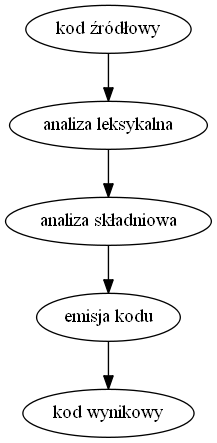
\includegraphics[width=5cm]{basic-compiler-flow}
    \caption{Podstawowy schemat budowy kompilatora}
    \label{basic_compiler_flow}
\end{figure}

Na rysunku \ref{basic_compiler_flow} przedstawiony jest uproszczony schemat budowy kompilatora.
W kompilatorach ''produkcyjnych'' (np. GCC, Clang, czy ICC) tych faz jest więcej -- przede wszystkim etap
emisji kodu jest dużo bardziej rozbudowany, oraz dochodzą etapy analizy semantycznej (czy program ma sens) czy
optymalizacji (prób takiego przekształcenia kodu programu żeby przy zachowaniu znaczenia działał wydajniej).

Kompilator języka ViuAct dostarczany jako element tej pracy inżynierskiej jest pozbawiony etapów
analizy semantycznej oraz optymalizacji. Analiza semantyczna (oraz weryfikacja typów i wykrywanie błędów na
etapie kompilacji) jest oddelegowana do assemblera dostarczanego przez platformę. Optymalizacja jest
całkowicie pominięta gdyż jest to temat niezwykle rozległy; implementacja i doszlifowanie algorytmów
optymalizujących kod jest sama w sobie materiałem wystarczającym na napisanie osobnej pracy inżynierskiej.

Architektura kompilatora języka ViuAct jest dokładniej opisana w rozdziale
\ref{architektura_kompilatora_viuact} (\nameref{architektura_kompilatora_viuact}) na
stronie \pageref{architektura_kompilatora_viuact}.
Sposób działania kompilatora jest opisany w rozdziale \ref{opis_etapow_kompilacji}
(\nameref{opis_etapow_kompilacji}) na stronie \pageref{opis_etapow_kompilacji}.
Omówienie interakcji kompilatora języka ViuAct z narzędziami dostarczanymi przez platformę Viua VM znajduje
się w rozdziale \ref{lang_architektura_systemu} (\nameref{lang_architektura_systemu}) na stronie
\pageref{lang_architektura_systemu}.

Oprócz kompilatora (rozdział \ref{opis_kompilatora} na stronie \pageref{opis_kompilatora}) dostarczany jest
również ''program łączący'' (rozdział \ref{opis_linkera} na stronie \pageref{opis_linkera}) dokonujący
automatycznego połączenia wymaganych modułów w gotowy plik wykonywalny.

\subsection{Architektura systemu}
\label{lang_architektura_systemu}

Rysunek \ref{schemat_interakcji_viuact_z_viuavm} (''\nameref{schemat_interakcji_viuact_z_viuavm}'') prezentuje
schemat interakcji jakie zachodzą w całym systemie od momentu wczytania pliku źródłowego przez kompilator do
uruchomienia programu przez jądro Viua VM.

Ostatnią fazą jaką zajmuje się kompilator języka ViuAct dostarczany jako element tej pracy inżynierskiej jest
emisja kodu (''Assembly code emission''), której wynikiem jest plik z kodem źródłowym w języku assemblera Viua
VM (''\texttt{hello\_world.asm}'' na rysunku \ref{schemat_interakcji_viuact_z_viuavm}).
Rozdział \ref{architektura_kompilatora_viuact} (\nameref{architektura_kompilatora_viuact}) dokładniej opisuje
działanie samego kompilatora.

\begin{figure}[!htp]
    \centering
    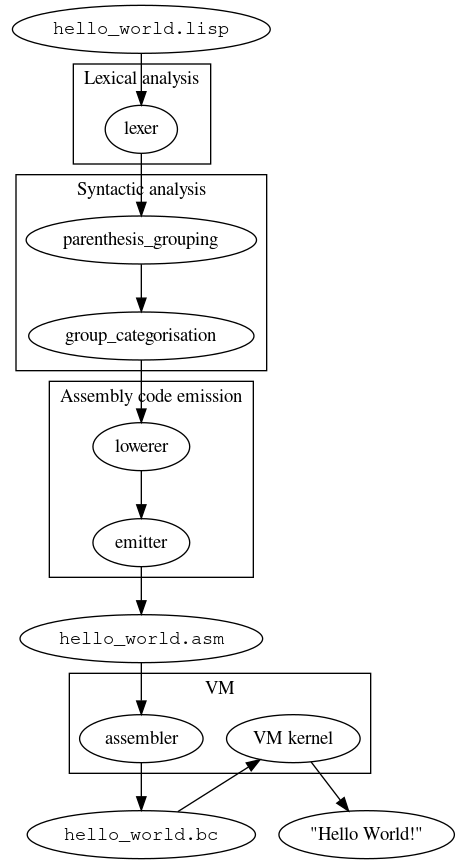
\includegraphics[width=9cm]{viuact-pipeline}
    \caption{Interakcje: od pliku źródłowego do działającego programu}
    \label{schemat_interakcji_viuact_z_viuavm}
\end{figure}

Zakres pracy inżynierskiej obejmuje wygenerowanie pliku zawierającego poprawny kod w języku
assemblera Viua VM oraz plików pomocniczych (zadanie kompilatora), oraz takim pokierowaniu
narzędziami dostarczanymi przez platformę, żeby wyemitowały one plik wykonywalny bądź bibliotekę (zadanie
''programu łączącego''). Zakładamy, że narzędzia dostarczane przez platformę działają poprawnie.

Pliki pomocnicze są wymagane przez ''program łączący'' (opisany w rozdziale \ref{opis_linkera} na stronie
\pageref{opis_linkera}). Ich dokładniejsze opisy znajdują się w rozdziałach
''\nameref{pliki_interfejsow_modulow}'' na stronie \pageref{pliki_interfejsow_modulow} i
''\nameref{pliki_zaleznosci_modulow}'' na stronie \pageref{pliki_zaleznosci_modulow}

\subsection{Dekompozycja systemu na podsystemy}
\label{architektura_kompilatora_viuact}

Język ViuAct jest implementowany przez dwa programy:

\begin{enumerate}
    \item \textbf{kompilator} - który przetwarza kod źródłowy w języku ViuAct na kod źródłowy w języku
        assemblera Viua VM
    \item \textbf{linker} - który na podstawie wyników pracy kompilatora tworzy pliki wykonywalne, które
        mogą być uruchomione na jądrze Viua VM
\end{enumerate}

Większość pracy w tym układzie wykonuje kompilator, opisany w rozdziale \ref{opis_kompilatora} na stronie
\pageref{opis_kompilatora}. Generuje on pliki zawierające kod źródłowy w języku assemblera gotowe do
przetworzenia przez assembler Viua VM na formę binarną, oraz pliki pomocnicze.

Z plików pomocniczych korzysta zarówno sam kompilator (do określenia interfejsów modułów importowanych przez
aktualnie kompilowany moduł), ale też linker -- do określenia jakie moduły powinny być dołączone do aktualnie
emitowanego pliku wykonywalnego, aby zapewnić dostępność wszystkich wymaganych funkcji. Linker jest dokładniej
opisany w rozdziale \ref{opis_linkera} na stronie \pageref{opis_linkera}.

\subsubsection{Kompilator -- \texttt{viuact-cc}}
\label{opis_kompilatora}

Kompilator składa się z kilku podsystemów, zgodnie z
przedstawieniem na rysunku \ref{ogolny_schemat_kompilatora_viuact}.

\begin{figure}[!htp]
    \centering
    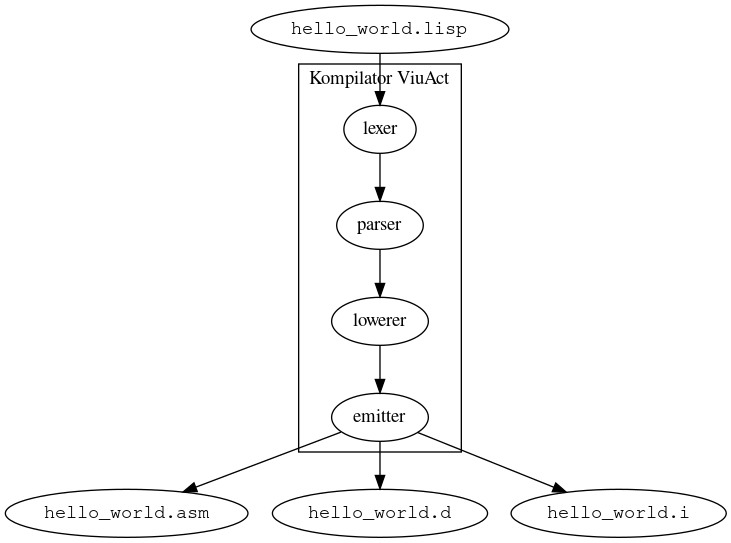
\includegraphics[width=10cm]{viuact-ogolny-schemat-kompilatora}
    \caption{Podział kompilatora na podsystemy}
    \label{ogolny_schemat_kompilatora_viuact}
\end{figure}

Każdy podsystem implementuje jedną z faz kompilacji:

\begin{enumerate}
    \item \textbf{lexer} dokonuje analizy leksykalnej wczytanego pliku źródłowego, dzieląc go na listę tokenów
    \item \textbf{parser} dokonuje analizy składniowej łącząc tokeny w grupy reprezentujące większe
        konstrukcje językowe
    \item \textbf{lowerer} mapuje grupy wyprodukowane przez \emph{parser} do odpowiednich funkcji
        \emph{emittera}; jest to dość banalny etap, ale upraszcza budowę kompilatora
    \item \textbf{emitter} tłumaczy konstrukcje językowe ViuAct na równoznaczne konstrukcje w języku
        assemblera Viua VM
\end{enumerate}

Różnica między podsystemami \emph{lowerer} i \emph{emitter} może być niejasna. Oba biorą udział w emisji
kodu wynikowego, ale \emph{lowerer} bezpośrednio zajmuje się tylko modułami i funkcjami, natomiast
\emph{emitter} implementuje emisję pojedynczych wyrażeń języka ViuAct -- przypisań \texttt{let}, konstrukcji
warunkowych \texttt{if}, wywołań funkcji, itd.

Proces kompilacji dokłaniej opisany jest w rozdziale \ref{opis_etapow_kompilacji}
(\nameref{opis_etapow_kompilacji}) na stronie \pageref{opis_etapow_kompilacji}.

\subsubsection{Program łączący -- \texttt{viuact-opt}}
\label{opis_linkera}

Program łączący (tzw. ,,\emph{linker}'') zajmuje się finalną fazą ,,kompilacji''.
Jest to stwierdzenie jednocześnie trafne i niepoprawne. Zazwyczaj jednak nie ma to znaczenia, ponieważ zarówno
linker jak i kompilator jest ukrywany przed programistą. Popularne ,,kompilatory'' jak np \emph{\texttt{g++}}
z GCC to tak naprawdę ,,drivery''; wywołanie polecenia \emph{\texttt{g++}} powoduje wywołanie zarówno
kompilatora (\emph{\texttt{cc1}}), assemblera (\emph{\texttt{as}}), jak i linkera (\emph{\texttt{ld}}) w taki
sposób aby na wyjściu uzyskać oczekiwany wynik, czyli na przykład plik wykonywalny w formacie
ELF \emph{\texttt{a.out}}.

W przypadku kompilatora ViuAct proces ten wygląda podobnie, ale nie jest aż tak zautomatyzowany.
Rolę ,,drivera'' pełni programista, który jest odpowiedzialny za wywołanie zarówno kompilatora jak i linkera.
Przykładowo:

\begin{lstlisting}
viuact-cc --mode exec ./hello_world.lisp
viuact-opt ./build/_default/hello_world.asm
\end{lstlisting}

Program łączący przeprowadzi proces asemblacji pliku podanego na wejściu, oraz dołączy do niego wszelkie
wymagane moduły. Zarówno asemblacja jak i łączenie będa przeprowadzone przez narzędzie dostarczane przez
platformę Viua VM -- \texttt{viuact-opt} zajmuje się jedynie wygenerowaniem odpowiednich poleceń dla tego
narzędzia.

Informacja o tym jakie moduły muszą zostać dołączone jest tworzona w oparciu o pliki zależności (opisane w
rozdziale \nameref{pliki_zaleznosci_modulow} na stronie \pageref{pliki_zaleznosci_modulow}).
Dla uproszczenia projektu program łączący nie zbiera informacji o zależnościach rekurencyjnie.

Po zebraniu informacji o zależnościach program łączący dokonuje asemblacji wszystkich modułów, od których
zależy kompilowany moduł główny. Następnie asembluje moduł główny i łączy wszystkie wyemitowane modułu
bytecode'u w gotowy plik wykonywalny.

\subsection{Przebieg procesu kompilacji}
\label{opis_etapow_kompilacji}

Ten rozdział zawiera dokładny opis procesu kompilacji, od momentu wczytania pliku z kodem źródłowym w języku
ViuAct do momentu wyemitowania kodu wynikowego w języku assemblera Viua VM. Kompilator jest wywoływany
poleceniem \texttt{viuact-cc} z opcją \texttt{-}\texttt{-mode} określającą czy kompilowany jest moduł wykonywalny
(\texttt{exec}) czy moduł biblioteki (\texttt{module}):

\begin{lstlisting}
viuact-cc --mode ( 'exec' | 'module' ) %*\emph{file.lisp}*)
\end{lstlisting}

\subsubsection{Wczytanie pliku źródłowego}

Kompilator wczytuje do pamięci cały plik źródłowy jako pojedynczy string.

\subsubsection{Analiza leksykalna}

Lexer patrzy na wczytany kod źródłowy i do pierwszego nieprzeanalizowanego znaku (czyli na początku analizy do
znaku na indeksie 0) próbuje przypasować wzorzec określający jaki token znajduje się na tej pozycji. Po udanym
przypasowaniu pozycja, która będzie rozpatrywana przez lexer jest przesuwana o tyle znaków ile wynosi długość
wygenerowanego tokenu i lexer rozpoczyna pracę od nowa. Ten proces trwa do momentu aż cały string wejściowy
nie zostanie przeanalizowany, albo odrzucony jako nieprawidłowy.

Algorytm przypasowania jest banalny. Lexer dysponuje listę wzorców (określonych przez wyrażenia regularne),
które określają jak wygląda każdy możliwy token w języku. Lexer po kolei próbuje przypasować każdy wzorzec z
listy i kończy na pierwszym trafieniu. Jeśli żaden wzorzec nie może zostać przypisany lexer odrzuca kod
źródłowy jako nieprawidłowy.

Wzorce są uszeregowane w taki sposób żeby nie była możliwa pomyłka i
na przykład przypasowanie początku nazwy zmiennej \texttt{letter} jako słowa kluczowego \texttt{let}.

\subsubsection{Analiza składniowa}
\label{opis_etapow_kompilacji_analiza_skladniowa}

Składnia języka została zaprojektowana w taki sposób aby analiza składniowa mogła być uproszczona do maksimum
i prosta w implementaji.

\paragraph{Grupowanie nawiasów}

W pierwszej fazie analizy składniowej tokeny grupowane są wegług nawiasów okrągłych, przy czym grupowanie jest
rekurencyjne (jeśli jakaś grupa zawiera podgrupę w nawiasach to zagnieżdżona grupa będzie widoczna jako
pojedynczy element w grupie zewnętrznej).
Dla przykładu:

\begin{lstlisting}
(let x (frobnicate 42))
\end{lstlisting}

będzie zgrupowane w następujący sposób:

\begin{lstlisting}
[ "let"; "x"; [ "frobnicate"; "42" ] ]
\end{lstlisting}

\paragraph{Grupowanie id}

Kolejnym etapem jest grupowanie id. Id jest nazwą składającą się z kilku członów, na przykład
\texttt{Std.Posix.Network.socket} składa się z 7 tokenów: trzech \emph{nazw modułów} (\texttt{Str},
\texttt{Posix}, i \texttt{Network}), trzech \emph{operatorów dostępu} (kropek), i jednej \emph{nazwy}
(\texttt{socket}).
Taka grupa zostanie na tym etapie zredukowana do pojedynczego elementu.

\paragraph{Oznczanie wyrażeń złożonych}

Wyrażenia złożone składają się z kilku wyrażeń (prostych bądź złożonych). Z uwagi na fakt, że formą pośrednią
wykorzystywaną na etapie grupowania są listy tokenów takie wyrażenie byłoby nieodróżnialne od listy
reprezentującej wywołanie funkcji. Dlatego na etapie analizy składniowej do list reprezentujących wyrażenia
złożone dodawany jest specjalny token-fantom. Dzięki temu zostaje zachowana właściwość umożliwiająca szybkie
klasyfikowanie grup. Dla przykładu:

\begin{lstlisting}
(let x { ... })
\end{lstlisting}

będzie zgrupowane w następujący sposób:

\begin{lstlisting}
[ "let"; "x"; [ Compound_expression_marker; ... ] ]
\end{lstlisting}

\paragraph{Klasyfikacja grup}

Ostatnim etapem analizy składniowej jest klasyfikacja grup. W większości przypadków do klasyfikacji listy
tokenów do grupy reprezentującej konkretną konstrukcję językową wystarczy spojrzeć na pierwszy token na
liście. W niektórych przypadkach algorytm musi się posiłkować długością listy.

Dla przykładu:

\begin{lstlisting}
[ "let"; "x";          ... ]        -> let-binding
[ "let"; "x"; [ ... ]; ... ]        -> function-definition
[ ... ]                             -> function-call
[ "actor"; ... ]                    -> actor-call
[ Compound_expression_marker; ... ] -> compound-call
\end{lstlisting}

Różnicą między definicją zmiennej (\texttt{let-binding}), a definicją funkcji (\texttt{function-definition})
jest długość listy - definicja zmiennej zawiera trzy elementy (słowo kluczowe \texttt{let}, nazwę, i
wyrażenie), a definicja funkcji cztery elementy (słowo kluczowe \texttt{let}, nazwę, listę parametrów
formalnych, i wyrażenie).

\subsubsection{Emisja modułów}

W następnej kolejności emitowane są wszystkie moduły zagnieżdżone w aktualnie kompilowanym module, przy czym
ten etap postępuje rekurencyjnie. Moduły zagnieżdżone musżą być wyemitowane przed modułem głównym, aby
kompilator miał dostęp do ich plików interfejsów i umożliwić ich importowanie.

\subsubsection{Analiza importu modułów}

Kolejnym krokiem jest analiza modułów importowanych przez aktualnie kompilowany moduł i wczytanie ich
interfejsów. Kompilator ładuje listy sygnatur funkcji i wyliczenia z każdego zaimportowanego modułu.

Jeśli kompilator nie może znaleźć pliku interfejsu danego modułu to kończy kompilację informując o błędzie.
Kompilator szuka plików interfejsów i modułów w ścieżkach podanych w zmiennej środowiskowej
\texttt{VIUAC\_LIBRARY\_PATH} (opisanej na stronie \pageref{viuact_manual_env_viuac_library_path}).

\subsubsection{Emisja kodu wynikowego}
\label{opis_etapow_kompilacji_emisja_kodu_wynikowego}

Na końcu następuje emisja kodu wynikowego w języku assemblera Viua VM. Ten etap jest wykonywany osobno dla
każdej funkcji zdefiniowanej w kompilowanym module.

\paragraph{Redukcja poziomu wyrażeń}

Najpierw następuje redukcja poziomu wyrażeń. Tym etapem zajmuje się \emph{lowerer}. Jest to mechaniczny proces
mapujący sklasyfikowane grupy reprezentujące konretne konstrukcje językowe do funkcji udostępnianych przez
\emph{emitter}, opakowanie wyniku w sposób jakiego wymagają zasady języka assemblera Viua VM, oraz
serializacja wyników do stringów.

\paragraph{Emisja instrukcji języka assemblera}

Emisja instrukcji języka assemblera jest wykonywana per-wyrażenie. Ten etap przeplata się z redukcją poziomu
wyrażeń i jest implementowany przez \emph{emitter}. \emph{Emitter} emituje sekwencje instrukcji języka
assemblera Viua VM odpowiadające zadanym konstrukcjom językowym ViuAct.

Dla przykładu \texttt{(let x 42)} zostanie wyemitowane jako pojedyncza instrukcja: \texttt{integer \%x local
42}.  Natomiast \texttt{(Some\_module.frobnicate 42)} zostanie wyemitowane jako sekwencja instrukcji:

\begin{lstlisting}
integer %3 local 42
frame %1 arguments
copy %0 arguments %3 local
call void Some_module::frobnicate/1
\end{lstlisting}

\subsubsection{Zapis pliku \texttt{.asm}}

Dla każdego wyemitowanego modułu kompilator zapisze plik \texttt{\emph{nazwa\_modulu}.asm} zawierający kod
wynikowy w języku assemblera Viua VM.

\subsubsection{Zapis pliku \texttt{.i}}

Dla każdego wyemitowanego modułu biblioteki kompilator zapisze plik \texttt{\emph{nazwa\_modulu}.i}
zawierający definicję interfejsu tego modułu. Pliki interfejsów są opisane w rozdziale
\nameref{pliki_interfejsow_modulow} na stronie \pageref{pliki_interfejsow_modulow}.

\subsubsection{Zapis pliku \texttt{.d}}

Dla każdego wyemitowanego modułu kompilator zapisze plik \texttt{\emph{nazwa\_modulu}.d}
zawierający definicję zależności tego modułu. Pliki zależności są opisane w rozdziale
\nameref{pliki_zaleznosci_modulow} na stronie \pageref{pliki_zaleznosci_modulow}.


\section{Projekt struktury}

\subsection{Wykorzystywane struktury danych}

Brak jest rozbudowanego diagramu klas, ponieważ program nie jest pisany w stylu obiektowym.
W programie istnieją dwie główne grupy struktur opisujące elementy języka -- typy tokenów i typy grup
(reprezentujących konstrukcje językowe), struktura reprezentująca adres rejestru (abstrakcyjny ,,slot'' na
wartości), struktura reprezentująca stan kompilowanego programu, oraz cztery struktury reprezentujące
niskopoziomowe abstrakcje linii programu w języku assemblera -- konstruktor, przeniesienie, wywołanie, i
,,\emph{verbatim}''.

\begin{quote}
    Listingi przedstawiające wykorzystywane struktury danych jest podany w języku OCaml.
    Kompilator jest napisany w języku Python, który nie pozwala na tak łatwe i czytelne definiowanie
    nowych struktur danych -- stąd decyzja o użyciu innego języka w pracy.

    Zachowane zostały typy danych, nazwy pól i całych struktur. OCaml pozwala na duże bardziej
    przejrzyste i czytelne opisanie typów danych poszczególnych pól niż Python, co ma dużą
    wartość dokumentacyjną.
\end{quote}

\subsubsection{Tokeny}
\label{diagram_klas_tokeny}

Każdy typ tokenu jest reprezentowany przez osobną strukturę. Tokeny, oprócz swojego typu mają atrybuty
określające ich lokalizację w pliku (wiersz i kolumna), oraz pole z leksemem. Typy tokenów wymagane do
reprezentacji języka ViuAct są opisane w specyfikacji języka.

Definicje struktur reprezentujących tokeny są zawarte w pliku \texttt{viuact/token\_types.py}.

\subsubsection{Grupy}
\label{diagram_klas_grupy}

Każda konstrukcja językowa jest reprezentowana przez osobną strukturę. Konstrukcje wymagane do reprezentacji
języka ViuAct są opisane w specyfikacji języka.

Definicje struktur reprezentujących grupy są zawarte w pliku \texttt{viuact/group\_types.py}.

\subsubsection{Slot}
\label{diagram_klas_slot}

\begin{lstlisting}
enum Register_set =
    | Local
    | Parameters
    | Arguments
    | Closure_local

type Slot = {
    name         : string ;
    index        : int ;
    register_set : register_set ;
}
\end{lstlisting}

Struktura \texttt{Slot} reprezentuje adres rejestru. Z punktu widzenia języka ViuAct istotne jest pole
\texttt{name} (określające nazwę slotu jaką posługuje się programista); z punktu widzenia emitera kodu istotne
są pola \texttt{index} i \texttt{register\_set} określające adres rejestru jakim posługuje się Viua VM.

\subsubsection{Stan programu}
\label{diagram_klas_stan_programu}

Stan programu (struktura \texttt{State}) zawiera pola śledzące ilość zaalokowanych rejestrów, widoczne
funkcje, a w przypadkach śledzenia stanu funkcji zagnieżdżonej -- także wykorzystywane sloty z otaczającego
zakresu leksykalnego.

\subsubsection{Konstruktor}
\label{diagram_klas_konstruktor}

\begin{lstlisting}
type Ctor = {
    of_type : string ;
    slot    : Slot ;
    value   : string ;
}
\end{lstlisting}

Konstruktor reprezentuje instrukcję bezpośrednio tworzącą wartość w rejestrze. Przykładowo, aby wyemitować
instrukcję \texttt{integer \%1 local 42} utworzony zostanie:

\begin{lstlisting}
{
    of_type = "integer" ;
    slot = { name = "x"; index = 1 ; Register_set.Local } ;
    value = "42"
}
\end{lstlisting}

\subsubsection{Przeniesienie}
\label{diagram_klas_przeniesienie}

\begin{lstlisting}
enum Move_kind =
    | Move
    | Copy

type Move = {
    kind   : Move_kind ;
    source : Slot ;
    dest   : Slot option ;
}
\end{lstlisting}

Przeniesienie opisuje przesunięcie (instrukcja \emph{\texttt{move}}) lub kopię wartości (instrukcja
\emph{\texttt{copy}}). Slot docelowy nie musi być obecny - np. wtedy wartość jest przenoszona do slotu
\texttt{void}.

\subsubsection{Wywołanie}
\label{diagram_klas_wywolanie}

\begin{lstlisting}
enum Call_kind =
    | Synchronous
    | Actor
    | Tail
    | Deferred

type Call = {
    kind : Call_kind ;
    slot : Slot option ;
    to   : string ;
}
\end{lstlisting}

Wywołanie opisuje wywołanie funkcji w każdy sposób dostępny w języku ViuAct: zwykłe wywołanie funkcji,
wywołanie tworzące aktora, wywołąnie \emph{tail call}, i wywołanie ''odroczone''.

Typy wywołań opisane są w specyfikacji języka.

\subsubsection{Linia ''\emph{verbatim}''}
\label{diagram_klas_linia_verbatim}

\begin{lstlisting}
type Verbatim = {
    text : string ;
}
\end{lstlisting}

Linia \emph{verbatim} opisuje dowolną linię języka assemblera (m.in. dyrektywy \texttt{.import:} czy
\texttt{.function:}).

\emph{Emitter} (rozdział \ref{opis_etapow_kompilacji_emisja_kodu_wynikowego} na stronie
\pageref{opis_etapow_kompilacji_emisja_kodu_wynikowego}) większość instrukcji tworzy za pomocą linii
\emph{verbatim}. Jest to zabieg o tyle ''brzydki'' co efektywny; na etapie prototypowania bardzo szybko
można w ten sposób wyemitować spory zakres instrukcji bez potrzeby projektowania struktury dla każdego typu
instrukcji.

\section{Decyzje projektowe}

\subsection{Środowisko docelowe}

Środowiskiem docelowym, na którym będą uruchamiane programy napisane w języku \ViuAct jest maszyna wirtualna
Viua VM. Środowisko docelowa musi spełniać wymagania jakie ma Viua VM (m.in. musi to być system zgodny ze
standardem POSIX).

\subsection{Środowisko implementacji}

Środowiskiem implmentacji jest Linux z dostępnymi standardowymi narzędziami GNU, językiem Python 3, i
umożliwiającym uruchomienie assemblera dostarczanego przez Viua VM.

\subsection{Priorytety implementacyjne}

Maksymalizacja prostoty budowy kompilatora i języka.
Marginalizacja obsługi błędów w kompilatorze z uwagi na brak czasu.
Marginalizacja optymalizacji z uwagi na brak czasu.

\section{Projekt algorytmów i przyjętych protokołów}

Dyskusja na temat algorytmów i sposobu implementacji jest częściowo przeprowadzona w rozdziale
\ref{opis_etapow_kompilacji} na stronie \pageref{opis_etapow_kompilacji}, szczególnie w rozdziale
\ref{opis_etapow_kompilacji_analiza_skladniowa}.

\section{Projekt rozwiązań sprzętowych}

Brak w tym projekcie. Jest on wyłącznie softwareowy.

\section{Projekt interfejsu}

\subsection{Interfejs użytkownika}

Interfejs użytkownika opisany jest w osobnym dokumencie -- podręczniku użytkownika kompilatora ViuAct (plik
''viuact-manual.pdf'').

\subsubsection{Założenia konstrukcji interfejsu}

\subsection{Interfejs kompilatora}

Kompilator składa się z dwóch programów: \texttt{viuact-cc} (kompilatora właściwego) i \texttt{viuact-opt}
(programu łączącego). Programy te są konfigurowane za pomocą zmiennych środowiskowych, które kontrolują poziom
''głośności'' logów, położenie assemblera Viua VM, a także włączają bądź wyłączają serializację formy
pośredniej.

Interfejs kompilatora opisany jest w osobnym dokumencie.

\subsection{Interfejs języka}

Interfejsem języka jest jego składnia.
Jest ona opisana w specyfikacji języka.

\subsection{Inne interfejsy}

\subsubsection{Pliki interfejsów modułów (\texttt{.i})}
\label{pliki_interfejsow_modulow}

Pliki interfejsów modułów wyliczają funkcje eksportowane przez dany moduł, oraz prezentują metadane wymagane
do połączenia plików w sposób, który będzie mógł działać na Viua VM. Pliki interfejsu dla modułów ''własnych''
nie różnią się zasadniczą strukturą od plików interfejsu dla modułów ''obcych'', ale pliki interfejsu dla
modułów ''obcych'' muszą być uzupełnione o kilka dodatkowych pól. Jest to dokładniej opisane w rozdziale
\ref{pliki_interfejsow_modulow_obcych} na stronie \pageref{pliki_interfejsow_modulow_obcych}.

Pliki interfejsów są zapisywane w formacie JSON.

\paragraph{Plik interfejsu dla modułów ''własnych''}

Moduły ''własne'' języka ViuAct to moduły napisane w języku ViuAct.

\begin{lstlisting}
{
    "foreign": false,
    "real_name": "A_module",
    "fns": [
        {
            "arity": 1,
            "name": "f",
            "real_name": "A_module::f",
            "from_module": "A_module"
        }
    ]
}
\end{lstlisting}

Atrybut \texttt{foreign} określa czy moduł jest ''obcy'' (\texttt{true}) czy ''własny'' (\texttt{false}).
Atrybut \texttt{real\_name} określa nazwę modułu tak jak będzie prezentowana na poziomie bytecode'u.
Atrybut \texttt{fns} jest listą funkcji, które są przez dany moduł eksportowane.

W elementach listy \texttt{fns} atrybuty mają następujące znaczenie:

\begin{enumerate}
    \item \texttt{arity} określa ''moc'' funkcji
    \item \texttt{name} określa nazwę funkcji widoczną z poziomu języka ViuAct
    \item \texttt{real\_name} określa pełną nazwę funkcji widoczną z poziomu bytecode'u
    \item \texttt{from\_module} określa pełną nazwę modułu, z którego pochodzi dana funkcja
\end{enumerate}

\paragraph{Plik interfejsu dla modułów ''obcych''}
\label{pliki_interfejsow_modulow_obcych}

Moduły ''obce'' języka ViuAct to moduły napisane w języku assemblera Viua VM lub w C++.

\begin{lstlisting}
{
    "foreign": true,
    "real_name": "std::posix::network",
    "fns": [
        {
            "arity": 0,
            "name": "socket",
            "real_name": "Std::Posix::Network::socket",
            "bytecode_name": "std::posix::network::socket",
            "from_module": "Std::Posix::Network"
        }
    ]
}
\end{lstlisting}

Różnicą w stosunku do plików interfejsu dla modułow ''własnych'' jest dodatkowy atrybut w deklaracji
eksportowanej funkcji -- \texttt{bytecode\_name} określający nazwę funkcji na poziomie bytecode'u. Nazwa ta
nie musi pokrywać się z nazwą w atrybucie \texttt{real\_name}, który określa pełną nazwę funkcji widoczną na
poziomie języka ViuAct.

Dwa atrybuty są potrzebne ponieważ na tym poziomie następuje łączenie dwóch ''światów''; języka ViuAct, który
narzuca reguły tego jak muszą wyglądać nazwy modułów i funkcji, oraz języka assemblera Viua VM, który takich
reguł nie narzuca. Dla modułów ''własnych'' atrybuty \texttt{bytecode\_name} jest zbędny ponieważ dla nich
nazwa widoczna na poziomie ViuAct i języka assemblera Viua VM jest taka sama.

\subsubsection{Pliki zależności modułów (\texttt{.d})}
\label{pliki_zaleznosci_modulow}

Pliki zależności są kodowane w formacie JSON.

\begin{lstlisting}
{
    "imports": [
        {
            "module_name": "Std::Random",
            "real_name": "std::random",
            "foreign": true
        }
    ]
}
\end{lstlisting}

Atrybut \texttt{imports} przechowuje listę modułów importowanych przez moduł, którego zależności definiuje
dany plik (co jest określane na podstawie nazwy pliku).

W elementach listy \texttt{imports} atrybuty mają następujące znaczenie:

\begin{enumerate}
    \item \texttt{module\_name} określa pełną nazwę modułu z punktu widzenia języka ViuAct
    \item \texttt{real\_name} określa pełną nazwę modułu widoczną z poziomu bytecode'u
    \item \texttt{foreign} określa czy moduł jest ''własny'' (\texttt{false}) czy ''obcy'' (\texttt{true})
\end{enumerate}

\section{Projekt bazy danych}

Brak bazy danych jako takiej w projekcie.
Dane przetwarzane przez kompilator są trzymane w plikach, których struktura opisana jest w rozdziałach
\ref{pliki_interfejsow_modulow} na stronie \pageref{pliki_interfejsow_modulow} i
\ref{pliki_zaleznosci_modulow} na stronie \pageref{pliki_zaleznosci_modulow}.

\section{Opis implementacji}

Implementacja kompilatora jest bardzo prosta, jak na standardy tego typu projektów.
Rysunek \ref{basic_compiler_flow} na stronie \pageref{basic_compiler_flow} bardzo dobrze oddaje strukturę
kompilatora dostarczonego jako wynik tej pracy.

\paragraph*{Analiza leksykalna i składniowa}
W fazie przygotowania tekstu programu ''do obróbki'' najpierw przeprowadzana jest analiza leksykalna (podział
tekstu na tokeny), później analiza składniowa -- która w dużej mierze polega na uporządkowaniu ''płaskiej''
listy tokenów w grupy ograniczone nawiasami. Algorytm dokonujący analizy składniowej jest trywialny:

\begin{enumerate}
    \item utwórz pustą listę przetworzoną
    \item rozważ token pierwszy nieprzenalizowany token
    \item jeśli ten token to \texttt{(} lub \texttt{\{}, rozpocznij rekurencyjnie przetwarzanie strumienia
        tokenów od następnego tokenu, a wynik analizy dodaj jako pojedynczy element do listy przetworzonej
    \item w innym przypadku dodaj token do listy przetworzonej
    \item jeśli na strumień tokenów jest pusty, zakończ algorytm
    \item w innym przypadku kontynuuj od punktu 2.
\end{enumerate}

Na pierwszy rzut oka widać, że ten algorytm nie analizuje wiele -- jego jedynym zadaniem jest pogrupowanie
płaskiego, jednowymiarowego strumienia tokenów w grupy reprezentujące konkretne konstrukcje językowe. Prostota
algorytmu sprawia, że jest on też bardzo szybki w działaniu.

Faktycznie, na tym etapie łączone są również rozbudowane identyfikatory (np. \texttt{foo.bar.baz}), ale nie
wpływa to znacząco na skomplikowanie kodu.

\paragraph*{Klasyfikacja grup}
Po tym etapie ''wstępnej'' analizy następuje klasyfikacja grup. W tym przypadku algorytm również jest bardzo
prosty. Klasyfikator rekurencyjnie sprawdza wszystkie listy i nadaje im typ oznaczający jaką konstrukcję
językową reprezentują. W tym celu musi jedynie sprawdzić typ pierwszego tokenu, i ewentualnie (w przypadku
dowiązań \emph{\texttt{let}} i definicji funkcji) długość listy.

Wykorzystanie algorytmu o tak niskim poziomie złożoności jest możliwe dzięki uważnemu zaprojektowaniu składni
języka. Każda konstrukcja językowa jest grupowana nawiasami -- klamrowymi bądź okrągłymi -- lub ma stałe
miejsce w grupie. Poniżej, dla przykładu, zaprezentowane są wzorce odpowiadające wybranym konstrukcjom
językowym:
\begin{lstlisting}
(let   %*\emph{name}*) %*\emph{expression}*))
(if    %*\emph{condition-expr}*) %*\emph{true-expr}*) %*\emph{false-expr}*))
(try   %*\emph{guarded-expr}*) ...)
(actor %*\emph{id}*) %*\emph{expr}*)*)
(+     %*\emph{lhs-expr}*) %*\emph{rhs-expr}*))
\end{lstlisting}

Jeśli całość oprócz pierwszego tokenu zostanie ''ukryta'' to dalej oczywistym jest z jaką konstrukcją mamy do
czynienia:
\begin{lstlisting}
(let   ...)
(if    ...)
(try   ...)
(actor ...)
(+     ...)
\end{lstlisting}

Wykorzystanie notacji polskiej (notacji prefiksowej) i takie zaprojektowanie składni, że każda konstrukcja ma
stałą ''szerokość'' pozwala na zastosowanie chwytu ''\emph{pierwszy token decyduje}''. Sprawia to też, że
język ma rozpoznawalne tempo i styl, a konsekwencja układu nadaje mu elegancji.


\section{Testowanie}

Testy kompilatora.

\subsection{Zestaw przypadków testowych}

Jeden testowy program na każdą funkcjonalność języka.
Kilka większych testowych programów sprawdzających integrację języka, np. wielomodułowych, wykorzystujących
moduły obce.

\subsection{Wykonanie testów}

Opis tego jak wygląda uruchomienie testów, w jaki sposób został zbudowany framework, itp.

\subsection{Trudności w testowaniu}

Niedeterminizm wynikający z równoległego działania aktorów stwarza problemy w testach. Trzeba uciekać się do
"sztuczek", np. sortowanie wyników programu testowego.

\section{Instrukcja użytkownika kompilatora języka Viuact}
\label{viuact_manual}

Tradycja nakazuje, aby pierwszym programem jaki pisze się w nowym języku był program, który wypisze na ekran
napis ,,\emph{Hello World!}''. W ViuAct ten program wygląda następująco:

\begin{lstlisting}
(let main () {
    (print "Hello World!")
    0
})
\end{lstlisting}

Aby skopilować ten program, należy wykonać w konsoli następujące polecenia:

\begin{lstlisting}
$ viuact-cc --mode exec ./hello_world.lisp
$ viuact-opt ./build/_default/hello_world.asm
\end{lstlisting}

Kod wykonywalny (\emph{bytecode} wykonywalny przez Viua VM) będzie umieszczony w pliku
\texttt{hello\_world.bc} w katalogu \texttt{./build/\_default}.
Aby go uruchomić należy użyć jądra Viua VM:

\begin{lstlisting}
$ viua-vm ./build/_default/hello_world.bc
%*\emph{Hello World!}*)
$
\end{lstlisting}

Nazwy plików pośrednich są wywodzone z nazwy pliku źródłowego:

\begin{description}
    \item[\texttt{\emph{example}.lisp}] plik z kodem źródłowym w języku ViuAct
    \item[\texttt{\emph{example}.asm}] plik wynikowy kompilatora, z kodem źródłowym w języku assemblera Viua
        VM
    \item[\texttt{\emph{example}.bc}] plik wynikowy assemblera Viua VM, zawierający wykonywalny bytecode
\end{description}

Pliki \texttt{.asm} i \texttt{.bc} są umieszczane w katalogu \texttt{./build/\_default}.

\subsection{Opcje kompilatora}

Jedyną opcją kompilatora jest \texttt{--mode}, która przyjmuje dwie możliwe wartości:

\begin{description}
    \item[\texttt{exec}] jeśli plik źródłowy definiuje moduł wykonywalny
    \item[\texttt{module}] jeśli plik źródłowy definiuje moduł biblioteczny
\end{description}

\subsection{Zmienne środowiskowe}

Zachowanie kompilatora można częściowo zmodyfikować ustawiając zmienne środowiskowe.

\subsubsection{\texttt{DEFAULT\_OUTPUT\_DIRECTORY}}

Kontroluje katalog, w którym kompilator składuje pliki wynikowe. Domyślnie pliki wynikowe są składowane w
katalogu \texttt{./build/\_default}.

\subsubsection{\texttt{VIUAC\_LIBRARY\_PATH}}

Jak \texttt{LD\_LIBRARY\_PATH}.

\subsubsection{\texttt{VIUA\_ASM\_PATH}}

Kontroluje ścieżkę do assemblera Viua VM.

\subsubsection{\texttt{VIUAC\_VERBOSE}}

Wartość \texttt{true} powoduje wyświetlenie komunikatów podczas kompilacji.

\subsubsection{\texttt{VIUAC\_DEBUGGING}}

Wartość \texttt{true} włącza komunikaty debugowania.

\subsubsection{\texttt{VIUAC\_INFO}}

Wartość \texttt{true} włącza dodatkowe komunikaty informacyjne.

\subsubsection{\texttt{VIUAC\_DUMP\_INTERMEDIATE}}

Wartość \texttt{tokens} powoduje zrzut strumienia tokenów do pliku \texttt{\emph{example}.tokens}.
Wartość \texttt{exprs} powoduje zrzut drzewa składni do pliku \texttt{\emph{example}.expressions}.
Można podać obie wartości, oddzielone przecinkiem.

\subsection{Opcje programu łączącego}


\chapter{Program ViuaChat -- formalności}

\section{Wprowadzenie}

\subsection{Cel dokumentu}
Celem dokumentu jest zdefiniowanie wymagań dla czatu ViuaChat na podstawie analizy otoczenia aplikacji oraz analizy potrzeb projektu w stosunku do niej.

\subsection{Zakres dokumentu}
Niniejszy dokument jest produktem pierwszego etapu procesu wytwórczego czatu ViuaChat, na który składają się:
\begin{itemize}
    \item analiza otoczenia, wraz z z klientami;
    \item wskazanie kontekstu biznesowego systemu;
    \item określenie udziałowców;
	\item wyszczególnienie i uporządkowanie zasad biznesowych, jakie zostały założone w stosunku do aplikacji;
	\item opracowanie historyjek na podstawie ustalonych zasad biznesowych.
\end{itemize}

\textbf{Uwaga:} Niniejszy dokument nie dotyczy języka ViuAct ani jego kompilatora.

\subsection{Dokumenty powiązane}
\begin{itemize}
	\item Szkic funkcjonalności ViuaChat - pierwszy zarys zasad biznesowych, ujęty w formie prostego konspektu;
	\item Specyfikacja wymagań biznesowych i \textit{user stories} - starsza wersja dokumentu SWS, nieujmująca otoczenia i kontekstu aplikacji.
\end{itemize}

\subsection{Odbiorcy}
Dokument został skierowany przede wszystkim dla członków zespołu, aby ułatwić im współpracę - w szczególności wówczas, gdy funkcjonalności czatu mogą pociągać za sobą modyfikację zestawu bibliotek ViuaVM bądź struktury składni projektowanego języka ViuAct.

Kolejną grupą adresatów niniejszego dokumentu są pracownicy uczelni, odpowiedzialni za nadzór nad prawidłowym ukształtowaniem i przebiegiem projektu. Wśród nich, szczególną rolę odgrywa JE Dziekan ZWI, prof. Marek Bednarczyk, będący opiekunem projektu.

\section{Czat w kontekście}

\subsection{Kontekst biznesowy}

Niniejszy czat stanowi część szerszego kontekstu, jakim jest potrzeba zademonstrowania działania języka ViuAct oraz całego środowiska wytwórczego powiązanego z maszyną wirtualną ViuaVM.

\begin{figure}[h]
	\centering
	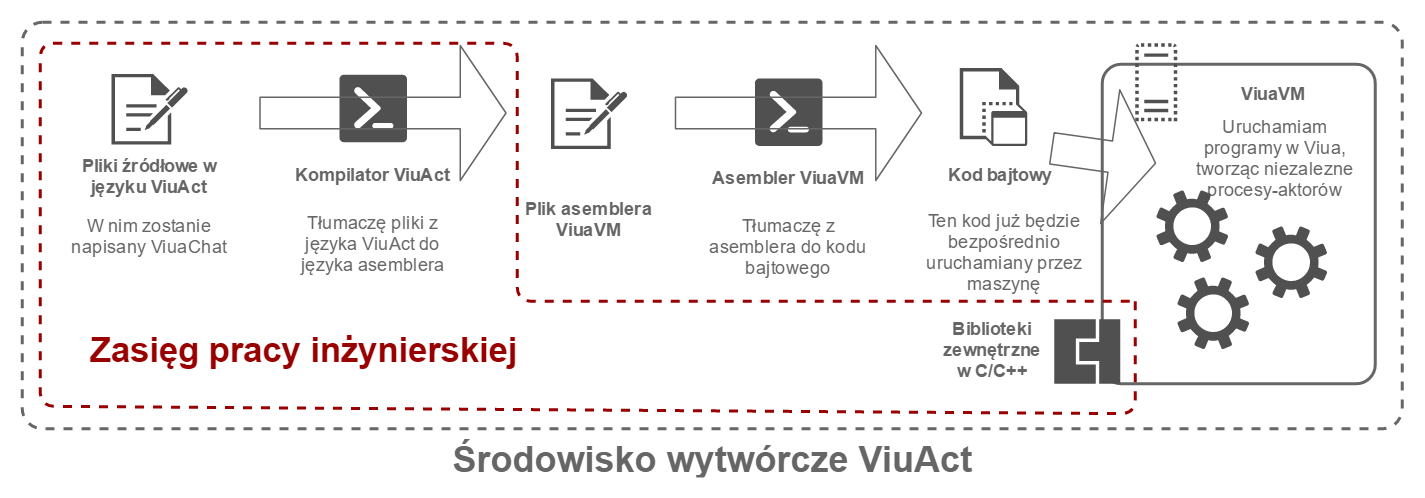
\includegraphics[width=\textwidth]{chat/fig/viuavm-env}
	\caption{Ilustracja środowiska wytwórczego wraz zasięgiem, którym są objęte prace przewidziane projektem inżynierskim}
\end{figure}

Cel demonstracyjny jest pierwszym i najważniejszym, jaki przyświeca konstrukcji czatu. Ponadto, sam proces wytwórczy pozwoli
przetestować wydajność całego środowiska w jego praktycznym wymiarze. Tym samym, możliwe będzie poprawienie konstrukcji kompilatora 
lub zastosowanych konstrukcji językowych ViuAct, podnoszących jego użyteczność.

Wszelcy odbiorcy dla aplikacji czatu zostaną, podobnie jak sama aplikacja, skonstruowani na cele demonstracyjne. Nie powinni oni
odbiegać od modelowych odbiorców podobnych komunikatorów, tak, aby potencjalny, poczatkujący użytkownik środowiska ViuaVM mógł
zrozumieć intencje stojące za rozwiązaniami zastosowanymi w ViuaChat oraz przenieść je do swoich pierwszych programów, opracowanych
w tym środowisku.

\subsection{Udziałowcy}

Poniżej wyszczególniono udziałowców, mających wpływ na rozwój czatu.

\begin{tabular}{ | l | l | }
  
	\hline
	\multicolumn{2}{ | l | }{\textbf{Karta udziałowca}}  \\
  
	\hline
    \parbox[t]{3cm}{
    	\textbf{Identyfikator}
    } & UN-01 \\  
    
    \hline
    \parbox[t]{3cm}{
    	\textbf{Nazwa}
    } & ViuaVM \\  
    
    \hline
    \parbox[t]{3cm}{
    	\textbf{Opis}
    } & \parbox[t]{12cm}{
    	Maszyna wirtualna, oparta o przechowywanie danych w rejestrach zamiast \textit{płaskich} tablic pamięci. Stanowi ona 
    	platformę, na której musi zostać uruchomiony serwer czatu. Ponieważ jej największym atutem jest zorientowanie na kod
    	wykonywany współbieżnie, sam serwer czatu powinien tę cechę wykorzystywać w maksymalnym stopniu. 
    	} \\ 
    
    \hline
    \parbox[t]{3cm}{
    	\textbf{Typ}
    } & Nieożywiony, bezpośredni \\  
    
    \hline
    \parbox[t]{3cm}{
    	\textbf{Punkt widzenia}
    } & \parbox[t]{12cm}{
    	ViuaVM jest absolutnie nieodzownym elementem projektu, a serwer czatu stanowi przede wszystkim dowód jej użyteczności.
    	O ile jądro maszyny nie ma być poddawane już żadnym zmianom i być wykorzystane takie, jakie było na inicjalnym etapie
    	pracy inżynierskiej, o tyle dopuszcza się poszerzanie jej funkcjonalności o dodatkowe biblioteki zewnętrzne.
    	} \\ 
    
    \hline
    \parbox[t]{3cm}{
    	\textbf{Ograniczenia}
    } & \parbox[t]{12cm}{
    	Maszyna wirtualna, jakkolwiek stanowi istotny czynnik dla decyzji w zakresie architektury czy konstrukcji oprogramowania,
    	nie powinna mieć wpływu na wymagania stricte biznesowe, jest bowiem jedynie środowiskiem do uruchamiania współbieżnych
    	programów, \textit{przezroczystym} dla końcowego użytkownika czy zleceniodawcy zrealizowanego oprogramowania.
    	} \\ 
    
    \hline
    \parbox[t]{3cm}{
    	\textbf{Wymagania}
    } & \colorbox{yellow}{...} \\ 
  
    \hline
\end{tabular}

\vspace{2em} 

\begin{tabular}{ | l | l | }

	\hline
	\multicolumn{2}{ | l | }{\textbf{Karta udziałowca}}  \\
  
	\hline
    \parbox[t]{3cm}{
    	\textbf{Identyfikator}
    } & UO-01 \\  
    
    \hline
    \parbox[t]{3cm}{
    	\textbf{Nazwa}
    } & Opiekun pracy inżynierskiej \\ 
    
    \hline
    \parbox[t]{3cm}{
    	\textbf{Opis}
    } & \parbox[t]{12cm}{
    	Pracownik uczelni, wyznaczony do opieki nad całym projektem inżynierskim - nadzorowania jego postępów, wskazywania problemów
    	oraz sugerowania decyzji podwyższających walor pracy oraz szanse na jej skuteczne obronienie. Ma również zasadniczy wpływ na 
    	decyzję o dopuszczeniu pracy do recenzji.
    } \\ 
    
    \hline
    \parbox[t]{3cm}{
    	\textbf{Typ}
    } & Ożywiony, bezpośredni \\  
    
    \hline
    \parbox[t]{3cm}{
    	\textbf{Punkt widzenia}
    } & \parbox[t]{12cm}{
    	Opiekun pracy patrzy na czat przede wszystkim przez pryzmat jego użyteczności jako efektownego przykładu implementacji modelu
    	aktora w praktycznym, programistycznym ujęciu. Stąd, jego uwaga skupia się przede wszystkim na konstrukcjach językowych,
    	strukturach oraz rozwiązaniach od strony kodu źródłowego. Czat stanowi jedynie pretekst do przeniesienia teoretycznych, akademickich
    	rozważań na praktyczny grunt. 
    	} \\ 
    
    \hline
    \parbox[t]{3cm}{
    	\textbf{Ograniczenia}
    } & \parbox[t]{12cm}{
    	Opiekun pracy, pomimo bycia jej nadzorcą i posiadania istotnych uprawnień decyzyjnych w stosunku do jej dalszego rozwoju, 
    	nie ma możliwości bieżącego śledzenia prac oraz
    	podejmowania decyzji w przypadku konkretnych problemów. Powinien zachować dystans, pozwalający na samodzielną realizację projektu
    	przez zespół. Stąd, jego faktyczny udział ogranicza się do udzielania porad w przypadku strategicznych kierunków, w jakich
    	będzie podążała grupa, a także doraźnego recenzowania ograniczonej puli zagadnień, wyłapanych w trakcie wspólnych spotkań.
    	} \\ 
    
    \hline
    \parbox[t]{3cm}{
    	\textbf{Wymagania}
    } & \colorbox{yellow}{...} \\ 
  
    \hline
\end{tabular}

\vspace{2em} 

\begin{tabular}{ | l | l | }

	\hline
	\multicolumn{2}{ | l | }{\textbf{Karta udziałowca}}  \\
  
	\hline
    \parbox[t]{3cm}{
    	\textbf{Identyfikator}
    } & UO-02 \\  
    
    \hline
    \parbox[t]{3cm}{
    	\textbf{Nazwa}
    } & \parbox[t]{12cm}{
    Członek zespołu ds. ViuAct
    } \\ 
    
    \hline
    \parbox[t]{3cm}{
    	\textbf{Opis}
    } & \parbox[t]{12cm}{
    	Student i członek zespołu, skupiający się w pierwszej kolejności nad rozwojem języka programowania ViuAct, jego kompilatora oraz
    	ewentualnego rozbudowania maszyny ViuaVM o kolejne, zewnętrzne biblioteki.
    } \\ 
    
    \hline
    \parbox[t]{3cm}{
    	\textbf{Typ}
    } & Ożywiony, bezpośredni \\  
    
    \hline
    \parbox[t]{3cm}{
    	\textbf{Punkt widzenia}
    } & \parbox[t]{12cm}{
    	Przede wszystkim, postrzega czat jako produkt, realizowany na końcowej platformie. Stąd, musi brać udział w formułowaniu
    	wymagań związanych z ViuaVM oraz językiem ViuAct. Jego zadaniem jest doprowadzenia do zaprojektowania czatu w sposób, 
    	który ukaże możliwości ViuAct jako solidnego, kompletnego rozwiązania. Przy tym, musi trzymać rękę na pulsie i reagować,
    	gdyby pojawiały się przeszkody w zaprogramowaniu czatu, wynikające z niedoskonałości środowiska wytwórczego.
    	
    	Podczas współudziału w definiowaniu wymagań, istotny jest dla niego zakres pracy, wiążący się z 
    	urzeczywistnianiem poszczególnych, proponowanych wymagań. Zbyt rozbudowany czat może opóźnić prace nad całym projektem,
    	a w efekcie - zniweczyć trud włożony w rozwój języka programowania i dedykowanego mu kompilatora.
    	} \\ 
    
    \hline
    \parbox[t]{3cm}{
    	\textbf{Ograniczenia}
    } & \parbox[t]{12cm}{
    	Jego udział w pracach nad czatem jest z gruntu nieograniczony. Jednakże, decydując się na podział odpowiedzialności 
    	podyktowany zespołowym charakterem projektu oraz własnymi ograniczeniami czasowymi, zrezygnował z decydowania o biznesowej 
    	części wymagań, faktycznie pozostając w roli konsultanta.
    	
    	} \\ 
    
    \hline
    \parbox[t]{3cm}{
    	\textbf{Wymagania}
    } & \colorbox{yellow}{...} \\ 
  
    \hline
\end{tabular}

\vspace{2em} 

\begin{tabular}{ | l | l | }

	\hline
	\multicolumn{2}{ | l | }{\textbf{Karta udziałowca}}  \\
  
	\hline
    \parbox[t]{3cm}{
    	\textbf{Identyfikator}
    } & UO-03 \\  
    
    \hline
    \parbox[t]{3cm}{
    	\textbf{Nazwa}
    } & \parbox[t]{12cm}{
    Członek zespołu ds. Czatu
    } \\ 
    
    \hline
    \parbox[t]{3cm}{
    	\textbf{Opis}
    } & \parbox[t]{12cm}{
    	Student i członek zespołu, odpowiedzialny za prace nad czatem
    } \\ 
    
    \hline
    \parbox[t]{3cm}{
    	\textbf{Typ}
    } & Ożywiony, bezpośredni \\  
    
    \hline
    \parbox[t]{3cm}{
    	\textbf{Punkt widzenia}
    } & \parbox[t]{12cm}{
    	Czat stanowi dla niego, obok dokumentacji, najistotniejszą część przedsięwzięcia. Musi z jednej strony nauczyć się poruszać
    	w nowym, dynamicznie zmieniającym się środowisku programistycznym, a z drugiej strony - zrealizować przy jego użyciu serwer
    	czatu, który pokaże jego możliwości i zastosowania innym nowicjuszom.
    	
    	Podczas współudziału w definiowaniu wymagań, istotny jest dla niego zakres końcowych funkcjonalności czatu. Nie może być zbyt 
    	wąski. Z drugiej strony, konstrukcja programu powinna pozostać prosta i przejrzysta. Przykładowy kod nie powinien odstraszać
    	potencjalnego programisty, dla którego cała koncepcja ViuaVM oraz modelu aktorów może wydawać się na pierwszy rzut oka nieco egzotyczna.
    	} \\ 
    
    \hline
    \parbox[t]{3cm}{
    	\textbf{Ograniczenia}
    } & \parbox[t]{12cm}{
    	Nie ma w zasadzie organizacyjnych czy kompetencyjnych ograniczeń dla formułowania wymagań. Nie oznacza to jednak, że może
    	definiować wymagań w oderwaniu od pozostałych udziałowców (ich role i punkty widzenia opisano wcześniej).
    	} \\ 
    
    \hline
    \parbox[t]{3cm}{
    	\textbf{Wymagania}
    } & \colorbox{yellow}{...} \\ 
  
    \hline
\end{tabular}

\subsection{Charakterystyka użytkowników}

Na etapie analizy kontekstu, w którym ma zostać zaprojektowany i zrealizowany czat, zadecydowano o zaprojektowaniu następujących,
modelowych użytkowników docelowego oprogramowania:

\begin{enumerate}

	\item \textbf{Użytkownik tymczasowy.} Typ użytkownika, którego konto jest tworzone podczas połączenia z serwerem czatu oraz 
		niszczone po jego zakończeniu. Podczas łączenia z czatem, nie będzie musiał się autoryzować przy użyciu hasła, a deklarować
		tylko unikalną nazwę, nie powtarzającą się z nazwą innego użytkownika, posiadającego konto na danym serwerze czatu. Ten typ
		konta jest przeznaczony dla osób, zainteresowanych dołączeniem do dyskusji na czacie bez dodatkowych zobowiązań.
		
	\item \textbf{Użytkownik stały.} Typ użytkownika, którego konto jest utrzymywane przez serwer pomiędzy połączeniami do czatu. W
		zamierzeniu, adresatami takiego rozwiązania mają być stali bywalcy serwera, którzy chcą mieć zarezerwowaną określoną nazwę
		dla siebie i uniknąć ewentualnego podszywania się. Stąd każdorazowo, przed rozpoczęciem sesji połączenia z serwerem, muszą się
		dodatkowo autoryzować przy użyciu hasła. Równocześnie, ich nazwa jest zarezerwowana wyłącznie do jego użytku oraz niedostępna
		dla użytkowników tymczasowych.
		
	\item \textbf{Administrator.} To użytkownik stały, który jest dodatkowo wyróżniony i posiada uprawienia do szeroko pojętego 
		zarządzania serwerem (w tym - pozostałymi użytkownikami). Nie wyróżnia się wśród administratorów żadnych dodatkowych, szczególnych
		ról (np. superadministrator, właściciel).
		
\end{enumerate}

Poza wspomnianymi różnicami, wszyscy użytkownicy po rozpoczęciu sesji połączenia mają prawo do dołączania do pokojów oraz wysyłania sobie
nawzajem wiadomości prywatnych. Łącznie, pula użytkowników przebywających na serwerze czatu w jednym momencie nie powinna przekraczać 320,
zaś w jednym pokoju - nie więcej niż 32. W związku z tym można przyjąć, że czat jest przeznaczony dla niewielkich społeczności, np.
szkolnych, uczelnianych czy hobbystycznych.

\subsection{Istniejąca infrastruktura}

\begin{itemize}
	\item \textbf{Komputer A}
	\begin{itemize}
		\item komputer przenośny z procesorem Intel Core i5 oraz systemem operacyjnym Windows 10
		\item XAMPP 7.2.7, obejmujący serwer Apache 2.4 oraz interpreter języka PHP w wersji 7.2.7.
	\end{itemize}
	
	\item \textbf{Komputer B}
	\begin{itemize}
		\item komputer przenośny, na którym zainstalowano system operacyjny Linux Mint 19 ,,Tara''
		\item GNU Compiler Collection 8.2
		\item wirtualna maszyna Viua VM w wersji 0.9.0
		\item \textit{należy doinstalować serwer Nginx, odpowiedzialny za wysłanie frontendu do
		użytkownika łączącego się z czatem oraz za handshake Websocketu}
	\end{itemize}
	
	\item \textit{\textbf{Do uzupełnienia}
	\begin{itemize}
		\item Kolejne urządzenie końcowe (trzecie), dzięki któremu będzie można symulować połączenie kolejnej
		osoby do usługi czatu
	\end{itemize}}

\end{itemize}

\section{Zasady biznesowe}

Zidentyfikowane zasady pogrupowano w 3 kategorie, biorąc pod uwagę podstawowe bloki funkcjonalności. Przydzielenie
do kategorii jest sygnalizowanie literą alfabetu, będącą prefiksem identyfikatora danej zasady. Dokonano
również priorytetyzacji zasad biznesowych według klasycznej skali ,,MoSCoW":

\begin{itemize}
	\item \textbf{,,M''} (z ang. \textit{must}) - zasady, których spełnienie jest niezbędne dla realizacji systemu
	\item \textbf{,,S''} (z ang. \textit{should}) - są to zasady o wysokim priorytecie, które powinny;
	zostać spełnione, o ile tylko jest to możliwe;
	\item \textbf{,,C''} (z ang. \textit{could}) - dobrze byłoby zrealizować takie wymagania, ale zależy to od czasu
	i zasobów, jakie pozostaną do dyspozycji po ukończeniu zadań ,,M" i ,,C";
	\item \textbf{,,W''} (z ang. \textit{won't}) - takie wymagania, po dyskusji, zostały wycofane dalszej realizacji.
\end{itemize}

\subsection{System użytkowników [ZU]}
  \begin{tabular}{ | l | l | l | }
	\hline
    \textbf{ID} & \parbox[t]{14cm}{
    	\textbf{Zasada biznesowa}
    } & \textbf{Priorytet} \\  
  
    \hline
    ZU-01 & \parbox[t]{14cm}{
      Podczas wejścia na czat, użytkownikowi pokazuje się monit z polem do wpisania nazwy użytkownika. 
    } & M \\

    \hline
    ZU-02 & \parbox[t]{14cm}{
      Użytkownicy bez stałego konta podczas logowania podają tylko nazwę użytkownika, pole hasła pozostaje puste .
    } & M \\

    \hline
    ZU-03 & \parbox[t]{14cm}{
      Nazwa użytkownika to ciąg od 3 do 32 alfanumerycznych znaków.
    } & M \\

    \hline
    ZU-04 & \parbox[t]{14cm}{
      Można rozpocząć sesję jako użytkownik, pod warunkiem, że zadeklarowana nazwa nie będzie powtarzać się z nazwami już zalogowanych użytkowników. 
    } & M \\

    \hline
    ZU-05 & \parbox[t]{14cm}{
      Monit podczas wejścia na czat jest wyposażony w pole do wpisania hasła (nieobowiązkowe). 
    } & S \\

    \hline
    ZU-06 & \parbox[t]{14cm}{
      Użytkownicy czatu ze stałym kontem, podczas logowania podają nazwę i odpowiadające mu hasło.
    } & S \\

    \hline
    ZU-07 & \parbox[t]{14cm}{
      Stałe konta użytkowników są utrzymywane na serwerze w postaci trójek wartości: nazwa użytkownika, hasło (md5), czy jest administratorem. 
    } & S \\

    \hline
    ZU-08 & \parbox[t]{14cm}{
      Nie można rozpocząć sesji użytkownika o nazwie, która pasuje do istniejącego konta, jeżeli nie zostanie podane prawidłowe hasło (nie można podszywać się pod nazwy użytkowników ze stałym kontem).
    } & S \\

    \hline
    ZU-09 & \parbox[t]{14cm}{
      Można rozpocząć sesję jako użytkownik bez podawania hasła, pod warunkiem, że zadeklarowana nazwa nie będzie powtarzać się z nazwami stałych kont użytkowników.
    } & S \\

    \hline
    ZU-10 & \parbox[t]{14cm}{
      W okienkach czatu, loginy użytkowników ze stałym kontem są pogrubione i pokolorowane: Administratorzy na czerwono,
      Pozostali na zielono. 
      } & S \\

    \hline
    ZU-11 & \parbox[t]{14cm}{
      Administratorzy mają prawo przeglądać nazwy pokojów na serwerze. 
    } & M \\

    \hline
    ZU-12 & \parbox[t]{14cm}{
      Administratorzy mają prawo tworzyć i usuwać pokoje. 
    } & S \\

    \hline
    ZU-13 & \parbox[t]{14cm}{
      Administratorzy mają prawo ustanawiać, zmieniać i usuwać hasła do pokojów. 
    } & C \\

    \hline
    ZU-14 & \parbox[t]{14cm}{
      Administratorzy mają prawo wyrzucać użytkowników z pokojów. 
    } & C \\

    \hline
    ZU-15 & \parbox[t]{14cm}{
      Administratorzy mają prawo wyrzucać użytkowników z serwera. 
    } & C \\

    \hline
    ZU-16 & \parbox[t]{14cm}{
      Administratorzy mają prawo przeglądać nazwy i poziomy uprawnień kont stałych użytkowników. 
    } & M \\

    \hline
    ZU-17 & \parbox[t]{14cm}{
      Administratorzy mają prawo tworzyć i usuwać użytkowników. 
    } & S \\

    \hline
    ZU-18 & \parbox[t]{14cm}{
      Administratorzy mają prawo zmieniać hasła użytkowników. 
    } & C \\

    \hline
    ZU-19 & \parbox[t]{14cm}{
      Administratorzy mają prawo zmieniać uprawnienia stałych kont użytkowników. 
    } & C \\

    \hline
    ZU-20 & \parbox[t]{14cm}{
      Użytkownicy ze stałymi kontami mogą zmieniać swoje hasło.
    } & W \\

    
    \hline
  \end{tabular}

\subsection{Pokoje [ZP]}
  \begin{tabular}{ | l | l | l | }
	\hline
    \textbf{ID} & \parbox[t]{14cm}{
    	\textbf{Zasada biznesowa}
    } & \textbf{Priorytet} \\  
    
    \hline
    ZP-01 & \parbox[t]{14cm}{
      Pokoje to właściwe czaty – tam użytkownicy mogą wejść i pisać do siebie nazwajem
    } & M \\

    \hline
    ZP-02 & \parbox[t]{14cm}{
      Każdy pokój ma unikalną nazwę będącą ciągiem alfanumerycznym od 3 do 32 znaków
    } & M \\

    \hline
    ZP-03 & \parbox[t]{14cm}{
      Lista pokojów jest widoczna dla każdego użytkownika po zalogowaniu się do serwera czatu
    } & M \\

    \hline
    ZP-04 & \parbox[t]{14cm}{
      Użytkownik może być równocześnie wpięty do jednego pokoju
    } & M \\

    \hline
    ZP-05 & \parbox[t]{14cm}{
      Wiadomość wysłana w pokoju jest widoczna w oknie pokoju dla wszystkich użytkowników podpiętych do tego pokoju
    } & M \\

    \hline
    ZP-06 & \parbox[t]{14cm}{
      Użytkownik może się samodzielnie wypiąć z pokoju, do którego jest wpięty
    } & S \\

    \hline
    ZP-07 & \parbox[t]{14cm}{
      Pokój może mieć ustanowione hasło, które użytkownik musi wpisać przed podpięciem się do niego
    } & C \\
    
    \hline
    ZP-08 & \parbox[t]{14cm}{
      Nowo wpięty użytkownik widzi 10 najnowszych wiadomości, 
      które zostały wysłane do pokoju tuż przed wpięciem
    } & S \\
    
    \hline
    ZP-09 & \parbox[t]{14cm}{
      Serwer czatu automatycznie wysyła do pokoju wiadomości, 
      zawierające powiadomienia o wydarzeniach związanych z
      pokojem, tzw. wiadomości systemowe
    } & S \\
    
    \hline
    ZP-10 & \parbox[t]{14cm}{
      Wiadomości systemowe są niepodpisane przez
      żadnego użytkownika i zapisane kursywą
   	} & C \\
   	
   	\hline
    ZP-11 & \parbox[t]{14cm}{
      Wiadomość systemowa zostaje wysłana podczas wpięcia się
      nowego użytkownika do pokoju
   	} & S \\
   	
   	\hline
    ZP-12 & \parbox[t]{14cm}{
      Wiadomość systemowa zostaje wysłana podczas wypięcia
      użytkownika z pokoju
   	} & S \\
   	
   	\hline
    ZP-13 & \parbox[t]{14cm}{
      Wiadomość systemowa zostaje wysłana, gdy użytkownik
      wpięty do pokoju traci połączenie z serwerem czatu
   	} & S \\
   	
   	\hline
    ZP-14 & \parbox[t]{14cm}{
      Wiadomość systemowa zostaje wysłana, gdy użytkownik
      zostaje wyrzucony z pokoju
   	} & S \\	
    
    \hline
    
  \end{tabular}

\subsection{Prywatne wiadomości [ZW]}
  \begin{tabular}{ | l | l | l | }
  	\hline
    \textbf{ID} & \parbox[t]{14cm}{
    	\textbf{Zasada biznesowa}
    } & \textbf{Priorytet} \\  
    
    \hline
    ZW-01 & \parbox[t]{14cm}{
      Wiadomości prywatne to wiadomości, które są wysyłane do
      konkretnego odbiorcy, innego niż nadawca. Są one widoczne
      wyłącznie dla nadawcy i odbiorcy takiej wiadomości
    } & M \\

    \hline
    ZW-02 & \parbox[t]{14cm}{
      Wiadomość prywatna może być wysłana z okna czatu pokoju – wiadomości prywatne nie są pokazywane wszystkim uczestnikom czatu, a jedynie użytkownikowi, do którego jest adresowana. 
    } & M \\

    \hline
    ZW-03 & \parbox[t]{14cm}{
      Aby wysłać wiadomość prywatną w oknie pokoju, należy poprzedzić ją znakiem \# i nazwą użytkownika, do którego jest kierowana wiadomość, oddzielona spacją od komunikatu, np.: „\#user Tajna wiadomość”.
    } & C \\

    \hline
    ZW-04 & \parbox[t]{14cm}{
      W oknie czatu pokoju dopuszczalne jest wysyłanie wiadomości prywatnych tylko tych użytkowników, którzy są do niego w danym momencie podpięci
    } & C \\

    \hline
    ZW-05 & \parbox[t]{14cm}{
      Próba wysłania wiadomości prywatnej w pokoju powinna zostać
      odrzucona przez serwer i zwrócić błąd w przypadku gdy:
      \begin{itemize}
      	\item Po znaku „\#” pojawi się od razu znak spacji lub nie
      	będzie żadnych znaków (nie zostanie podana 
		nazwa użytkownika który jest adresatem)
		\item Nazwa adresata jest dłuższa niż 32 znaki
		\item Wysyłamy wiadomość prywatną w pokoju czatu do
		użytkownika, który nie jest podpięty do tego pokoju
      \end{itemize}
		
    } & M \\
    
    \hline
    ZW-06 & \parbox[t]{14cm}{
      Użytkownik dysponuje dedykowanym oknem, w którym widzi wiadomości prywatne. 
    } & M \\
    
    \hline
    ZW-07 & \parbox[t]{14cm}{
      Z okna wiadomości prywatnych można odbierać i wysyłać wyłącznie
      wiadomości prywatne, których nadawcą/odbiorcą jest wybrany
      użytkownik
    } & M \\    
    
    \hline
    ZW-08 & \parbox[t]{14cm}{
      W oknie wiadomości prywatnych można przeglądać wiadomości wysłane do i odebrane od jednego, wybranego użytkownika.
      
    } & S \\
    
    \hline
    ZW-09 & \parbox[t]{14cm}{
      W oknie wiadomości prywatnych można wysyłać wiadomości
      wyłącznie do nadawcy, którego wiadomości są w danym momencie
      pokazywane.
    } & S \\
    
    \hline
    ZW-10 & \parbox[t]{14cm}{
      Czas istnienia wiadomości prywatnych zależy od typu użytkownika
      który jest jej nadawcą i odbiorcą:
      \begin{itemize}
      	\item Jeżeli co najmniej jedna strona komunikacji
      	 jest użytkownikiem tymczasowym, wiadomości są
      	 utrzymywane dopóki nadawca i odbiorca nie skończą
      	 sesji na serwerze
      	\item Jeżeli jedna strona komunikacji jest
      	użytkownikiem
      	tymczasowym, a druga stałym, to wiadomość jest utrzymywana
      	dopóki użytkownik tymczasowy skończy sesję połączenia z
      	serwerem
      	\item Jeżeli obie strony są użytkownikami stałymi, to
      	wiadomość jest trzymana bezterminowo
      \end{itemize}
    } & S \\
    
    \hline
    ZW-11 & \parbox[t]{14cm}{
      Dla każdej pary użytkowników, na serwerze jest
      gromadzone co najwyżej 100 wiadomości prywatnych.
    } & S \\
    \hline
  \end{tabular}

\section{Wymagania}
\label{program_viuachat_wymagania}

\subsection{Wymagania funkcjonalne}

Ponieważ obraną metodologią wytwarzania aplikacji jest \textit{mini-Scrum}, należący do kategorii metodyk zwinnych, wymagania funkcjonalne ujęto w formie historyjek (\textit{user stories}).

\vspace{2em} 

\begin{tabular}{ | l | l | }
	\hline
		\textbf{Identyfikator} & 
		WF-01
		\\
		
	\hline
		\textbf{Treść} & \parbox[t]{11cm}{
			Jako użytkownik serwera czatu, chcę się do niego zalogować, aby zobaczyć listę pokojów dyskusyjnych.
		}\\
		 
	\hline
		\parbox[t]{4cm}{\textbf{Powiązane zasady biznesowe}} & \parbox[t]{11cm}{
			ZU-01 Podczas wejścia na czat, użytkownikowi pokazuje się monit z polem do wpisania nazwy użytkownika. \\
			ZP-03 Lista pokojów jest widoczna dla każdego użytkownika
			po zalogowaniu się do serwera czatu
		}\\
		
	\hline
		\parbox[t]{4cm}{\textbf{Kryteria akceptacji}} & \parbox[t]{11cm}{
			\begin{enumreq}
				\item Po wejściu na czat bez rozpoczętej sesji, pokazuje się monit o podanie nazwy użytkownika.
				\item Po wpisaniu nazwy użytkownika i zatwierdzeniu, użytkownik rozpocznie sesję na serwerze czatu.
				\item Tuż po rozpoczęciu sesji czatu, użytkownik zobaczy listę pokojów.
			\end{enumreq}
			}
		\\

	\hline
\end{tabular}

\vspace{2em} 

\begin{tabular}{ | l | l | }
	\hline
		\textbf{Identyfikator} & 
		WF-02
		\\
		
	\hline
		\textbf{Treść} & \parbox[t]{11cm}{
			Jako użytkownik serwera czatu, chcę wpiąć się do pokoju,
			aby wziąć udział w dyskusji.
		}\\
		 
	\hline
		\parbox[t]{4cm}{\textbf{Powiązane zasady biznesowe}} & \parbox[t]{11cm}{
			ZP-01 Pokoje to właściwe czaty - tam użytkownicy mogą
			wejść i pisać do siebie nawzajem
		}\\
		
	\hline
		\parbox[t]{4cm}{\textbf{Kryteria akceptacji}} & \parbox[t]{11cm}{
			\begin{enumreq}
				\item Użytkownik, który ma otwartą sesję 
				połączenia z serwerem czatu i nie jest wpięty
				do żadnego pokoju, zobaczy listę pokojów.
				\item Użytkownik, po kilknięciu w liście pokojów
				na nazwę pokoju, zostanie do niego podpięty
				\item Użytkownik po wpięciu się do pokoju zobaczy
				okno pokoju
				\item Użytkownik, który ma otwartą sesję
				połączenia z serwerem i jest wpięty do pokoju,
				po odświeżeniu przeglądarki zobaczy okno pokoju, 
				do którego jest wpięty
			\end{enumreq}
			}
		\\

	\hline
\end{tabular}

\vspace{2em} 

\begin{tabular}{ | l | l | }
	\hline
		\textbf{Identyfikator} & 
		WF-03
		\\
		
	\hline
		\textbf{Treść} & \parbox[t]{11cm}{
			Jako użytkownik serwera czatu, chcę po wpięciu
			do pokoju zobaczyć ostatnie wiadomości wysłane
			przed moim dołączeniem, aby dowiedzieć się, co
			tam się obecnie dzieje.
		}\\
		 
	\hline
		\parbox[t]{4cm}{\textbf{Powiązane zasady biznesowe}} & \parbox[t]{11cm}{
			ZP-08 Nowo wpięty użytkownik widzi 10 najnowszych
			wiadomości, które zostały wysłane do pokoju tuż
			przed wpięciem
		}\\
		
	\hline
		\parbox[t]{4cm}{\textbf{Kryteria akceptacji}} & \parbox[t]{11cm}{
			\begin{enumreq}
				\item Użytkownik po wpięciu się do pokoju zobaczy
				10 najnowszych wiadomości wysłanych do pokoju
				przed jego dołączeniem (lub mniej, jeżeli
				dotychczas nie wysłano do pokoju co najmniej
				10 wiadomości)
			\end{enumreq}
			}
		\\

	\hline
\end{tabular}

\vspace{2em} 

\begin{tabular}{ | l | l | }
	\hline
		\textbf{Identyfikator} & 
		WF-04
		\\
		
	\hline
		\textbf{Treść} & \parbox[t]{11cm}{
			Jako użytkownik serwera czatu, chcę chcę wysłać
			wiadomość do pokoju w który jestem wpięty, aby
			zobaczyli ją inni uczestnicy dyskusji.
		}\\
		 
	\hline
		\parbox[t]{4cm}{\textbf{Powiązane zasady biznesowe}} & \parbox[t]{11cm}{
			ZP-01 Pokoje to właściwe czaty - tam użytkownicy mogą
			wejść i pisać do siebie nawzajem
		}\\
		
	\hline
		\parbox[t]{4cm}{\textbf{Kryteria akceptacji}} & \parbox[t]{11cm}{
			\begin{enumreq}
				\item Użytkownik wpisze tekst wiadomości w polu
				tekstowym u dołu czatu
				\item Wiadomość wpisana w polu tekstowym zostanie
				wysłana po wciśnięciu klawisza ,,Enter'', gdy aktywne
				będzie pole tekstowe
				\item Wiadomość wpisana w polu tekstowym zostanie
				wysłana po naciśnięciu przycisku ,,Wyślij'',
				widocznego obok pola tekstowego
				\item Po wysłaniu wiadomości, pole tekstowe zostanie
				wyczyszczone (niezależnie od tego czy wiadomość
				zostanie doręczona)
				\item Wiadomość wysłana do pokoju jest pokazywana
				wszystkim użytkownikom podpiętym do czatu u dołu
				strony
				\item Nowa wiadomość jest pokazywana wraz z nazwą
				użytkownika wysyłającego u dołu konwersacji
			\end{enumreq}
			}
		\\

	\hline
\end{tabular}

\vspace{2em} 

\begin{tabular}{ | l | l | }
	\hline
		\textbf{Identyfikator} & 
		WF-05
		\\
		
	\hline
		\textbf{Treść} & \parbox[t]{11cm}{
			Jako użytkownik serwera czatu, chcę chcę zobaczyć
			powiadomienie o wpięciu się nowego użytkownika do
			pokoju w którym sam jestem obecnie wpięty, aby powitać
			nowego dyskutanta
		}\\
		 
	\hline
		\parbox[t]{4cm}{\textbf{Powiązane zasady biznesowe}} & \parbox[t]{11cm}{
			ZP-09 Serwer czatu automatycznie wysyła do pokoju
			wiadomości, zawierające powiadomienia o wydarzeniach
			związanych z pokojem, tzw. wiadomości systemowe \\
			ZP-11 Wiadomość systemowa zostaje wysłana podczas
			wpięcia się nowego użytkownika do pokoju
		}\\
		
	\hline
		\parbox[t]{4cm}{\textbf{Kryteria akceptacji}} & \parbox[t]{11cm}{
			\begin{enumreq}
				\item Niezwłocznie po wpięciu się użytkownika do
				pokoju, serwer wyśle wiadomość systemową o treści
				,,Użytkownik ... dołączył do pokoju'', widoczną
				dla wszystkich użytkowników wpiętych do tego pokoju
			\end{enumreq}
			}
		\\

	\hline
\end{tabular}

\vspace{2em} 

\begin{tabular}{ | l | l | }
	\hline
		\textbf{Identyfikator} & 
		WF-06
		\\
		
	\hline
		\textbf{Treść} & \parbox[t]{11cm}{
			Jako użytkownik serwera czatu, chcę zobaczyć
			powiadomienie o opuszczeniu pokoju przez użytkownika,
			aby łatwo zorientować się, że nie bierze już udziału 
			w dyskusji.
		}\\
		 
	\hline
		\parbox[t]{4cm}{\textbf{Powiązane zasady biznesowe}} & \parbox[t]{11cm}{
			ZP-09 Serwer czatu automatycznie wysyła do pokoju
			wiadomości, zawierające powiadomienia o wydarzeniach
			związanych z pokojem, tzw. wiadomości systemowe \\
			ZP-12 Wiadomość systemowa zostaje wysłana podczas
			wpięcia wypięcia użytkownika z pokoju \\
			ZP-13 Wiadomość systemowa zostaje wysłana, gdy użytkownik
			wpięty do pokoju traci połączenie z serwerem \\
			ZP-14 Wiadomość systemowa zostaje wysłana, gdy użytkownik
			zostaje wyrzucony z pokoju
			
		}\\
		
	\hline
		\parbox[t]{4cm}{\textbf{Kryteria akceptacji}} & \parbox[t]{11cm}{
			\begin{enumreq}
				\item Niezwłocznie po wypięciu się użytkownika z
				pokoju, serwer wyśle wiadomość systemową, widoczną
				dla wszystkich użytkowników wpiętych do tego pokoju,
				o treści:
				\begin{enumerate}
					\item ,,Użytkownik ... opuścił pokój'', gdy
					użytkownik samodzielnie wypiął się z pokoju
					\item ,,Użytkownik ... stracił połączenie'',
					gdy użytkownik został wypięty z pokoju na skutek
					przerwania sesji z uwagi na zerwanie połączenia
					\item ,,Użytkownik ... został wyrzucony'', gdy
					użytkownik został wypięty wskutek interwencji
					administratora
				\end{enumerate}
			\end{enumreq}
			}
		\\

	\hline
\end{tabular}

\vspace{2em} 

\begin{tabular}{ | l | l | }
	\hline
		\textbf{Identyfikator} & 
		WF-07
		\\
		
	\hline
		\textbf{Treść} & \parbox[t]{11cm}{
			Jako użytkownik serwera czatu, chcę odpiąć się od pokoju,
			aby wpiąć się do innego pokoju.
		}\\
		 
	\hline
		\parbox[t]{4cm}{\textbf{Powiązane zasady biznesowe}} & \parbox[t]{11cm}{
			ZP-06 Użytkownik może się samodzielnie wypiąć z pokoju,
			do którego jest wpięty
			
		}\\
		
	\hline
		\parbox[t]{4cm}{\textbf{Kryteria akceptacji}} & \parbox[t]{11cm}{
			\begin{enumreq}
				\item W oknie pokoju użytkownik zobaczy przycisk
				lub link ,,Opuść pokój''.
				\item Po kliknięciu w ,,Opuść pokój'', użytkownik
				zobaczy listę pokojów.
			\end{enumreq}
			}
		\\

	\hline
\end{tabular}

\vspace{2em} 

\begin{tabular}{ | l | l | }
	\hline
		\textbf{Identyfikator} & 
		WF-08
		\\
		
	\hline
		\textbf{Treść} & \parbox[t]{11cm}{
			Jako użytkownik serwera czatu, chcę zobaczyć
			okno wiadomości prywatnych, aby odczytać wiadomości,
			które wysłano specjalnie do mnie.
		}\\
		 
	\hline
		\parbox[t]{4cm}{\textbf{Powiązane zasady biznesowe}} & \parbox[t]{11cm}{
			ZW-01 Wiadomości prywatne to wiadomości, które są
			wysyłane do konkretnego odbiorcy, innego niż
			nadawca... \\
			ZW-06 Użytkownik dysponuje dodatkowym oknem, na którym
			widzi wiadomości prywatne. \\
			ZW-07 Z okna wiadomości prywatnych można odbierać i
			wysyłać wyłącznie wiadomości prywatne, których
			nadawcą / odbiorcą jest wybrany użytkownik. \\
		}\\
		
	\hline
		\parbox[t]{4cm}{\textbf{Kryteria akceptacji}} & \parbox[t]{11cm}{
			\begin{enumreq}
				\item Po kliknięciu w link ,,PW'', użytkownik
				zobaczy okno prywatnych wiadomości
				\item W oknie wiadomości prywatnych, użytkownik
				zobaczy listę użytkowników, od których otrzymał
				wiadomości prywatne.
				\item Po kliknięciu w link z nazwą użytkownika,
				użytkownik zobaczy prywatne wiadomości, których
				nadawcą i odbiorcą jest wskazana osoba.
			\end{enumreq}
			}
		\\

	\hline
\end{tabular}

\vspace{2em} 

\begin{tabular}{ | l | l | }
	\hline
		\textbf{Identyfikator} & 
		WF-09
		\\
		
	\hline
		\textbf{Treść} & \parbox[t]{11cm}{
			Jako użytkownik serwera czatu, chcę wysłać
			wiadomość prywatną do jednego użytkownika, aby
			prowadzić z nim ciągłą konwersację.
		}\\
		 
	\hline
		\parbox[t]{4cm}{\textbf{Powiązane zasady biznesowe}} & \parbox[t]{11cm}{
			
			
		}\\
		
	\hline
		\parbox[t]{4cm}{\textbf{Kryteria akceptacji}} & \parbox[t]{11cm}{
			\begin{enumreq}
				\item Użytkownik wpisze tekst wiadomości w polu
				tekstowym u dołu okna wiadomości prywatnych
				\item Wiadomość wpisana w polu tekstowym zostanie
				wysłana po wciśnięciu klawisza ,,Enter'', gdy
				aktywne
				będzie pole tekstowe
				\item Wiadomość wpisana w polu tekstowym zostanie
				wysłana po naciśnięciu przycisku ,,Wyślij'',
				widocznego obok pola tekstowego
				\item Po wysłaniu wiadomości, pole tekstowe zostanie
				wyczyszczone (niezależnie od tego czy wiadomość
				zostanie doręczona)
				\item Wiadomość wysłana w oknie zostanie pokazana
				tylko użytkownikowi, z którym trwa otwarta
				konwersacja
				\item Nowa wiadomość jest pokazywana wraz z nazwą
				użytkownika wysyłającego u dołu konwersacji
			\end{enumreq}`								
			}
		\\

	\hline
\end{tabular}


\vspace{2em} 

\begin{tabular}{ | l | l | }
	\hline
		\textbf{Identyfikator} & 
		WF-10
		\\
		
	\hline
		\textbf{Treść} & \parbox[t]{11cm}{
			Jako użbytkownik czatu, chcę wysłać wiadomość
			prywatną w oknie czatu, aby zobaczył ją tylko jej
			odbiorca
		}\\
		 
	\hline
		\parbox[t]{4cm}{\textbf{Powiązane zasady biznesowe}} & \parbox[t]{11cm}{
			
			
		}\\
		
	\hline
		\parbox[t]{4cm}{\textbf{Kryteria akceptacji}} & \parbox[t]{11cm}{
			\begin{enumreq}
				\item Użytkownik wpisze w oknie pokoju 
				wiadomość zapoczątkowaną znakiem kratki \# i nazwą 
				użytkownika obecnego na czacie, oddzieloną spacją 
				od treści wiadomości
				tekstowym u dołu okna wiadomości prywatnych
				\item Wiadomość wysłana w oknie zostanie pokazana
				tylko użytkownikowi, do którego została skierowana
				a także u tego użytkownika, który ją nadał
				\item Wiadomości prywatna w oknie pokoju jest
				podświetlona na żółto.
			\end{enumreq}`								
			}
		\\

	\hline
\end{tabular}


\vspace{2em} 

\begin{tabular}{ | l | l | }
	\hline
		\textbf{Identyfikator} & 
		WF-11
		\\
		
	\hline
		\textbf{Treść} & \parbox[t]{11cm}{
			Jako użytkownik serwera czatu, chcę wysłać wiadomość 
			prywatną do innego użytkownika, z którym wcześniej nie
			wymieniałem takich wiadomości, aby rozpocząć z nim
			prywatną konwersację.
		}\\
		 
	\hline
		\parbox[t]{4cm}{\textbf{Powiązane zasady biznesowe}} & \parbox[t]{11cm}{
			
			
		}\\
		
	\hline
		\parbox[t]{4cm}{\textbf{Kryteria akceptacji}} & \parbox[t]{11cm}{
			\begin{enumreq}
				\item Użytkownik kliknie w oknie wiadomości
				prywatnych w przyciski ,,Nowy''.
				\item Użytkownik zobaczy monit o podanie nazwy
				użytkownika, z którym chce rozpocząć rozmowę
				\item Jeżeli użytkownik jest aktywny, wówczas 
				\item Wiadomość wpisana w polu tekstowym zostanie
				wysłana po wciśnięciu klawisza ,,Enter'', gdy
				aktywne
				będzie pole tekstowe
				\item Wiadomość wpisana w polu tekstowym zostanie
				wysłana po naciśnięciu przycisku ,,Wyślij'',
				widocznego obok pola tekstowego
				\item Po wysłaniu wiadomości, pole tekstowe zostanie
				wyczyszczone (niezależnie od tego czy wiadomość
				zostanie doręczona)
				\item Wiadomość wysłana w oknie zostanie pokazana
				tylko użytkownikowi, z którym trwa otwarta
				konwersacja
				\item Nowa wiadomość jest pokazywana wraz z nazwą
				użytkownika wysyłającego u dołu konwersacji
			\end{enumreq}`								
			}
		\\

	\hline
\end{tabular}

\subsection{Wymagania niefunkcjonalne}

\begin{tabular}{ | l | l | }
	\hline
		\textbf{Identyfikator} & 
		HN-1
		\\
		
	\hline
		\textbf{Treść} & \parbox[t]{13cm}{
			Długość nazwy użytkownika jest ograniczona od 2 do 32 znaków alfanumerycznych, w celu uniknięcia problemów z identyfikacją użytkownika na serwerze.
		}\\
		 
	\hline
		\parbox[t]{4cm}{\textbf{Powiązane zasady biznesowe}} & \parbox[t]{13cm}{
			U-3 Nazwa użytkownika to ciąg od 3 do 32 alfanumerycznych znaków.
		}\\
		
	\hline
		\parbox[t]{4cm}{\textbf{Kryteria akceptacji}} & \parbox[t]{13cm}{
			\begin{enumreq}
				\item Po wpisaniu do pola użytkownika nazwy krótszej niż 2 znaki, dłużej niż 32 znaki lub zawierającej inne znaki niż alfanumeryczne, zwracany jest błąd.
			\end{enumreq}
			}
		\\

	\hline
\end{tabular}

\subsection{Wymagania na środowisko docelowe}

\begin{tabular}{ | l | l | }
	\hline
		\textbf{Identyfikator} & 
	WS-01
		\\
		
	\hline
		\textbf{Treść} & \parbox[t]{13cm}{
			W rozwiązaniu należy wykorzystać środowisko ViuaVM i
			język Viuact
		}\\

	\hline
\end{tabular}

\begin{tabular}{ | l | l | }
	\hline
		\textbf{Identyfikator} & 
	WS-02
		\\
		
	\hline
		\textbf{Treść} & \parbox[t]{13cm}{
			Czat będzie użytkowany jako aplikacja webowa typu
			\textit{single page application}
		}\\

	\hline
\end{tabular}

\begin{tabular}{ | l | l | }
	\hline
		\textbf{Identyfikator} & 
	WS-03
		\\
		
	\hline
		\textbf{Treść} & \parbox[t]{13cm}{
			Aplikacja czatu będzie dostosowana przede wszystkim
			do obsługi z wykorzystaniem urządzeń mobilnych.
		}\\

	\hline
\end{tabular}

\subsection{Wymagania dotyczące procesu wytwarzania}

\begin{tabular}{ | l | l | }
	\hline
		\textbf{Identyfikator} & 
	WW-01
		\\
		
	\hline
		\textbf{Treść} & \parbox[t]{13cm}{
			W procesie wytwórczym należy korzystać z metodologii
			mini-Scrum
		}\\

	\hline
\end{tabular}


\chapter{Program ViuaChat}
\label{program_viuachat}

Drugą częścią naszej pracy jest program ViuaChat - chat internetowy o funkcjonalności podobnej do IRC.
Umożliwia użytkownikom logowanie się do sieci, zakładanie pokojów tematycznych do rozmów, oraz rozmowy
''prywatne'' (tj. wyłączne dla dwóch użytkowników).

\section{Projekt struktury}

\subsection{Wykorzystywane struktury danych}

Brak jest rozbudowanego diagramu klas, ponieważ program nie jest pisany w stylu obiektowym.
W programie istnieją dwie główne grupy struktur opisujące elementy języka -- typy tokenów i typy grup
(reprezentujących konstrukcje językowe), struktura reprezentująca adres rejestru (abstrakcyjny ,,slot'' na
wartości), struktura reprezentująca stan kompilowanego programu, oraz cztery struktury reprezentujące
niskopoziomowe abstrakcje linii programu w języku assemblera -- konstruktor, przeniesienie, wywołanie, i
,,\emph{verbatim}''.

\begin{quote}
    Listingi przedstawiające wykorzystywane struktury danych jest podany w języku OCaml.
    Kompilator jest napisany w języku Python, który nie pozwala na tak łatwe i czytelne definiowanie
    nowych struktur danych -- stąd decyzja o użyciu innego języka w pracy.

    Zachowane zostały typy danych, nazwy pól i całych struktur. OCaml pozwala na duże bardziej
    przejrzyste i czytelne opisanie typów danych poszczególnych pól niż Python, co ma dużą
    wartość dokumentacyjną.
\end{quote}

\subsubsection{Tokeny}
\label{diagram_klas_tokeny}

Każdy typ tokenu jest reprezentowany przez osobną strukturę. Tokeny, oprócz swojego typu mają atrybuty
określające ich lokalizację w pliku (wiersz i kolumna), oraz pole z leksemem. Typy tokenów wymagane do
reprezentacji języka ViuAct są opisane w specyfikacji języka.

Definicje struktur reprezentujących tokeny są zawarte w pliku \texttt{viuact/token\_types.py}.

\subsubsection{Grupy}
\label{diagram_klas_grupy}

Każda konstrukcja językowa jest reprezentowana przez osobną strukturę. Konstrukcje wymagane do reprezentacji
języka ViuAct są opisane w specyfikacji języka.

Definicje struktur reprezentujących grupy są zawarte w pliku \texttt{viuact/group\_types.py}.

\subsubsection{Slot}
\label{diagram_klas_slot}

\begin{lstlisting}
enum Register_set =
    | Local
    | Parameters
    | Arguments
    | Closure_local

type Slot = {
    name         : string ;
    index        : int ;
    register_set : register_set ;
}
\end{lstlisting}

Struktura \texttt{Slot} reprezentuje adres rejestru. Z punktu widzenia języka ViuAct istotne jest pole
\texttt{name} (określające nazwę slotu jaką posługuje się programista); z punktu widzenia emitera kodu istotne
są pola \texttt{index} i \texttt{register\_set} określające adres rejestru jakim posługuje się Viua VM.

\subsubsection{Stan programu}
\label{diagram_klas_stan_programu}

Stan programu (struktura \texttt{State}) zawiera pola śledzące ilość zaalokowanych rejestrów, widoczne
funkcje, a w przypadkach śledzenia stanu funkcji zagnieżdżonej -- także wykorzystywane sloty z otaczającego
zakresu leksykalnego.

\subsubsection{Konstruktor}
\label{diagram_klas_konstruktor}

\begin{lstlisting}
type Ctor = {
    of_type : string ;
    slot    : Slot ;
    value   : string ;
}
\end{lstlisting}

Konstruktor reprezentuje instrukcję bezpośrednio tworzącą wartość w rejestrze. Przykładowo, aby wyemitować
instrukcję \texttt{integer \%1 local 42} utworzony zostanie:

\begin{lstlisting}
{
    of_type = "integer" ;
    slot = { name = "x"; index = 1 ; Register_set.Local } ;
    value = "42"
}
\end{lstlisting}

\subsubsection{Przeniesienie}
\label{diagram_klas_przeniesienie}

\begin{lstlisting}
enum Move_kind =
    | Move
    | Copy

type Move = {
    kind   : Move_kind ;
    source : Slot ;
    dest   : Slot option ;
}
\end{lstlisting}

Przeniesienie opisuje przesunięcie (instrukcja \emph{\texttt{move}}) lub kopię wartości (instrukcja
\emph{\texttt{copy}}). Slot docelowy nie musi być obecny - np. wtedy wartość jest przenoszona do slotu
\texttt{void}.

\subsubsection{Wywołanie}
\label{diagram_klas_wywolanie}

\begin{lstlisting}
enum Call_kind =
    | Synchronous
    | Actor
    | Tail
    | Deferred

type Call = {
    kind : Call_kind ;
    slot : Slot option ;
    to   : string ;
}
\end{lstlisting}

Wywołanie opisuje wywołanie funkcji w każdy sposób dostępny w języku ViuAct: zwykłe wywołanie funkcji,
wywołanie tworzące aktora, wywołąnie \emph{tail call}, i wywołanie ''odroczone''.

Typy wywołań opisane są w specyfikacji języka.

\subsubsection{Linia ''\emph{verbatim}''}
\label{diagram_klas_linia_verbatim}

\begin{lstlisting}
type Verbatim = {
    text : string ;
}
\end{lstlisting}

Linia \emph{verbatim} opisuje dowolną linię języka assemblera (m.in. dyrektywy \texttt{.import:} czy
\texttt{.function:}).

\emph{Emitter} (rozdział \ref{opis_etapow_kompilacji_emisja_kodu_wynikowego} na stronie
\pageref{opis_etapow_kompilacji_emisja_kodu_wynikowego}) większość instrukcji tworzy za pomocą linii
\emph{verbatim}. Jest to zabieg o tyle ''brzydki'' co efektywny; na etapie prototypowania bardzo szybko
można w ten sposób wyemitować spory zakres instrukcji bez potrzeby projektowania struktury dla każdego typu
instrukcji.

\section{Decyzje projektowe}

\subsection{Środowisko docelowe}

Środowiskiem docelowym, na którym będą uruchamiane programy napisane w języku \ViuAct jest maszyna wirtualna
Viua VM. Środowisko docelowa musi spełniać wymagania jakie ma Viua VM (m.in. musi to być system zgodny ze
standardem POSIX).

\subsection{Środowisko implementacji}

Środowiskiem implmentacji jest Linux z dostępnymi standardowymi narzędziami GNU, językiem Python 3, i
umożliwiającym uruchomienie assemblera dostarczanego przez Viua VM.

\subsection{Priorytety implementacyjne}

Maksymalizacja prostoty budowy kompilatora i języka.
Marginalizacja obsługi błędów w kompilatorze z uwagi na brak czasu.
Marginalizacja optymalizacji z uwagi na brak czasu.

\section{Projekt algorytmów i przyjętych protokołów}

Dyskusja na temat algorytmów i sposobu implementacji jest częściowo przeprowadzona w rozdziale
\ref{opis_etapow_kompilacji} na stronie \pageref{opis_etapow_kompilacji}, szczególnie w rozdziale
\ref{opis_etapow_kompilacji_analiza_skladniowa}.

\section{Projekt rozwiązań sprzętowych}

Brak w tym projekcie. Jest on wyłącznie softwareowy.

\section{Projekt interfejsu}

\subsection{Interfejs użytkownika}

Interfejs użytkownika opisany jest w osobnym dokumencie -- podręczniku użytkownika kompilatora ViuAct (plik
''viuact-manual.pdf'').

\subsubsection{Założenia konstrukcji interfejsu}

\subsection{Interfejs kompilatora}

Kompilator składa się z dwóch programów: \texttt{viuact-cc} (kompilatora właściwego) i \texttt{viuact-opt}
(programu łączącego). Programy te są konfigurowane za pomocą zmiennych środowiskowych, które kontrolują poziom
''głośności'' logów, położenie assemblera Viua VM, a także włączają bądź wyłączają serializację formy
pośredniej.

Interfejs kompilatora opisany jest w osobnym dokumencie.

\subsection{Interfejs języka}

Interfejsem języka jest jego składnia.
Jest ona opisana w specyfikacji języka.

\subsection{Inne interfejsy}

\subsubsection{Pliki interfejsów modułów (\texttt{.i})}
\label{pliki_interfejsow_modulow}

Pliki interfejsów modułów wyliczają funkcje eksportowane przez dany moduł, oraz prezentują metadane wymagane
do połączenia plików w sposób, który będzie mógł działać na Viua VM. Pliki interfejsu dla modułów ''własnych''
nie różnią się zasadniczą strukturą od plików interfejsu dla modułów ''obcych'', ale pliki interfejsu dla
modułów ''obcych'' muszą być uzupełnione o kilka dodatkowych pól. Jest to dokładniej opisane w rozdziale
\ref{pliki_interfejsow_modulow_obcych} na stronie \pageref{pliki_interfejsow_modulow_obcych}.

Pliki interfejsów są zapisywane w formacie JSON.

\paragraph{Plik interfejsu dla modułów ''własnych''}

Moduły ''własne'' języka ViuAct to moduły napisane w języku ViuAct.

\begin{lstlisting}
{
    "foreign": false,
    "real_name": "A_module",
    "fns": [
        {
            "arity": 1,
            "name": "f",
            "real_name": "A_module::f",
            "from_module": "A_module"
        }
    ]
}
\end{lstlisting}

Atrybut \texttt{foreign} określa czy moduł jest ''obcy'' (\texttt{true}) czy ''własny'' (\texttt{false}).
Atrybut \texttt{real\_name} określa nazwę modułu tak jak będzie prezentowana na poziomie bytecode'u.
Atrybut \texttt{fns} jest listą funkcji, które są przez dany moduł eksportowane.

W elementach listy \texttt{fns} atrybuty mają następujące znaczenie:

\begin{enumerate}
    \item \texttt{arity} określa ''moc'' funkcji
    \item \texttt{name} określa nazwę funkcji widoczną z poziomu języka ViuAct
    \item \texttt{real\_name} określa pełną nazwę funkcji widoczną z poziomu bytecode'u
    \item \texttt{from\_module} określa pełną nazwę modułu, z którego pochodzi dana funkcja
\end{enumerate}

\paragraph{Plik interfejsu dla modułów ''obcych''}
\label{pliki_interfejsow_modulow_obcych}

Moduły ''obce'' języka ViuAct to moduły napisane w języku assemblera Viua VM lub w C++.

\begin{lstlisting}
{
    "foreign": true,
    "real_name": "std::posix::network",
    "fns": [
        {
            "arity": 0,
            "name": "socket",
            "real_name": "Std::Posix::Network::socket",
            "bytecode_name": "std::posix::network::socket",
            "from_module": "Std::Posix::Network"
        }
    ]
}
\end{lstlisting}

Różnicą w stosunku do plików interfejsu dla modułow ''własnych'' jest dodatkowy atrybut w deklaracji
eksportowanej funkcji -- \texttt{bytecode\_name} określający nazwę funkcji na poziomie bytecode'u. Nazwa ta
nie musi pokrywać się z nazwą w atrybucie \texttt{real\_name}, który określa pełną nazwę funkcji widoczną na
poziomie języka ViuAct.

Dwa atrybuty są potrzebne ponieważ na tym poziomie następuje łączenie dwóch ''światów''; języka ViuAct, który
narzuca reguły tego jak muszą wyglądać nazwy modułów i funkcji, oraz języka assemblera Viua VM, który takich
reguł nie narzuca. Dla modułów ''własnych'' atrybuty \texttt{bytecode\_name} jest zbędny ponieważ dla nich
nazwa widoczna na poziomie ViuAct i języka assemblera Viua VM jest taka sama.

\subsubsection{Pliki zależności modułów (\texttt{.d})}
\label{pliki_zaleznosci_modulow}

Pliki zależności są kodowane w formacie JSON.

\begin{lstlisting}
{
    "imports": [
        {
            "module_name": "Std::Random",
            "real_name": "std::random",
            "foreign": true
        }
    ]
}
\end{lstlisting}

Atrybut \texttt{imports} przechowuje listę modułów importowanych przez moduł, którego zależności definiuje
dany plik (co jest określane na podstawie nazwy pliku).

W elementach listy \texttt{imports} atrybuty mają następujące znaczenie:

\begin{enumerate}
    \item \texttt{module\_name} określa pełną nazwę modułu z punktu widzenia języka ViuAct
    \item \texttt{real\_name} określa pełną nazwę modułu widoczną z poziomu bytecode'u
    \item \texttt{foreign} określa czy moduł jest ''własny'' (\texttt{false}) czy ''obcy'' (\texttt{true})
\end{enumerate}

\section{Projekt bazy danych}

Brak bazy danych jako takiej w projekcie.
Dane przetwarzane przez kompilator są trzymane w plikach, których struktura opisana jest w rozdziałach
\ref{pliki_interfejsow_modulow} na stronie \pageref{pliki_interfejsow_modulow} i
\ref{pliki_zaleznosci_modulow} na stronie \pageref{pliki_zaleznosci_modulow}.

\section{Opis implementacji}

Implementacja kompilatora jest bardzo prosta, jak na standardy tego typu projektów.
Rysunek \ref{basic_compiler_flow} na stronie \pageref{basic_compiler_flow} bardzo dobrze oddaje strukturę
kompilatora dostarczonego jako wynik tej pracy.

\paragraph*{Analiza leksykalna i składniowa}
W fazie przygotowania tekstu programu ''do obróbki'' najpierw przeprowadzana jest analiza leksykalna (podział
tekstu na tokeny), później analiza składniowa -- która w dużej mierze polega na uporządkowaniu ''płaskiej''
listy tokenów w grupy ograniczone nawiasami. Algorytm dokonujący analizy składniowej jest trywialny:

\begin{enumerate}
    \item utwórz pustą listę przetworzoną
    \item rozważ token pierwszy nieprzenalizowany token
    \item jeśli ten token to \texttt{(} lub \texttt{\{}, rozpocznij rekurencyjnie przetwarzanie strumienia
        tokenów od następnego tokenu, a wynik analizy dodaj jako pojedynczy element do listy przetworzonej
    \item w innym przypadku dodaj token do listy przetworzonej
    \item jeśli na strumień tokenów jest pusty, zakończ algorytm
    \item w innym przypadku kontynuuj od punktu 2.
\end{enumerate}

Na pierwszy rzut oka widać, że ten algorytm nie analizuje wiele -- jego jedynym zadaniem jest pogrupowanie
płaskiego, jednowymiarowego strumienia tokenów w grupy reprezentujące konkretne konstrukcje językowe. Prostota
algorytmu sprawia, że jest on też bardzo szybki w działaniu.

Faktycznie, na tym etapie łączone są również rozbudowane identyfikatory (np. \texttt{foo.bar.baz}), ale nie
wpływa to znacząco na skomplikowanie kodu.

\paragraph*{Klasyfikacja grup}
Po tym etapie ''wstępnej'' analizy następuje klasyfikacja grup. W tym przypadku algorytm również jest bardzo
prosty. Klasyfikator rekurencyjnie sprawdza wszystkie listy i nadaje im typ oznaczający jaką konstrukcję
językową reprezentują. W tym celu musi jedynie sprawdzić typ pierwszego tokenu, i ewentualnie (w przypadku
dowiązań \emph{\texttt{let}} i definicji funkcji) długość listy.

Wykorzystanie algorytmu o tak niskim poziomie złożoności jest możliwe dzięki uważnemu zaprojektowaniu składni
języka. Każda konstrukcja językowa jest grupowana nawiasami -- klamrowymi bądź okrągłymi -- lub ma stałe
miejsce w grupie. Poniżej, dla przykładu, zaprezentowane są wzorce odpowiadające wybranym konstrukcjom
językowym:
\begin{lstlisting}
(let   %*\emph{name}*) %*\emph{expression}*))
(if    %*\emph{condition-expr}*) %*\emph{true-expr}*) %*\emph{false-expr}*))
(try   %*\emph{guarded-expr}*) ...)
(actor %*\emph{id}*) %*\emph{expr}*)*)
(+     %*\emph{lhs-expr}*) %*\emph{rhs-expr}*))
\end{lstlisting}

Jeśli całość oprócz pierwszego tokenu zostanie ''ukryta'' to dalej oczywistym jest z jaką konstrukcją mamy do
czynienia:
\begin{lstlisting}
(let   ...)
(if    ...)
(try   ...)
(actor ...)
(+     ...)
\end{lstlisting}

Wykorzystanie notacji polskiej (notacji prefiksowej) i takie zaprojektowanie składni, że każda konstrukcja ma
stałą ''szerokość'' pozwala na zastosowanie chwytu ''\emph{pierwszy token decyduje}''. Sprawia to też, że
język ma rozpoznawalne tempo i styl, a konsekwencja układu nadaje mu elegancji.


\section{Diagramy Przypadków Użycia}

\subsection{Diagram Przypadków Użycia}

Diagram przypadków użycia jest pokazany na rysunku \ref{dpu-chat-v2}
\nameref{dpu-chat-v2}.
\begin{figure}[!htp]
	\centering
	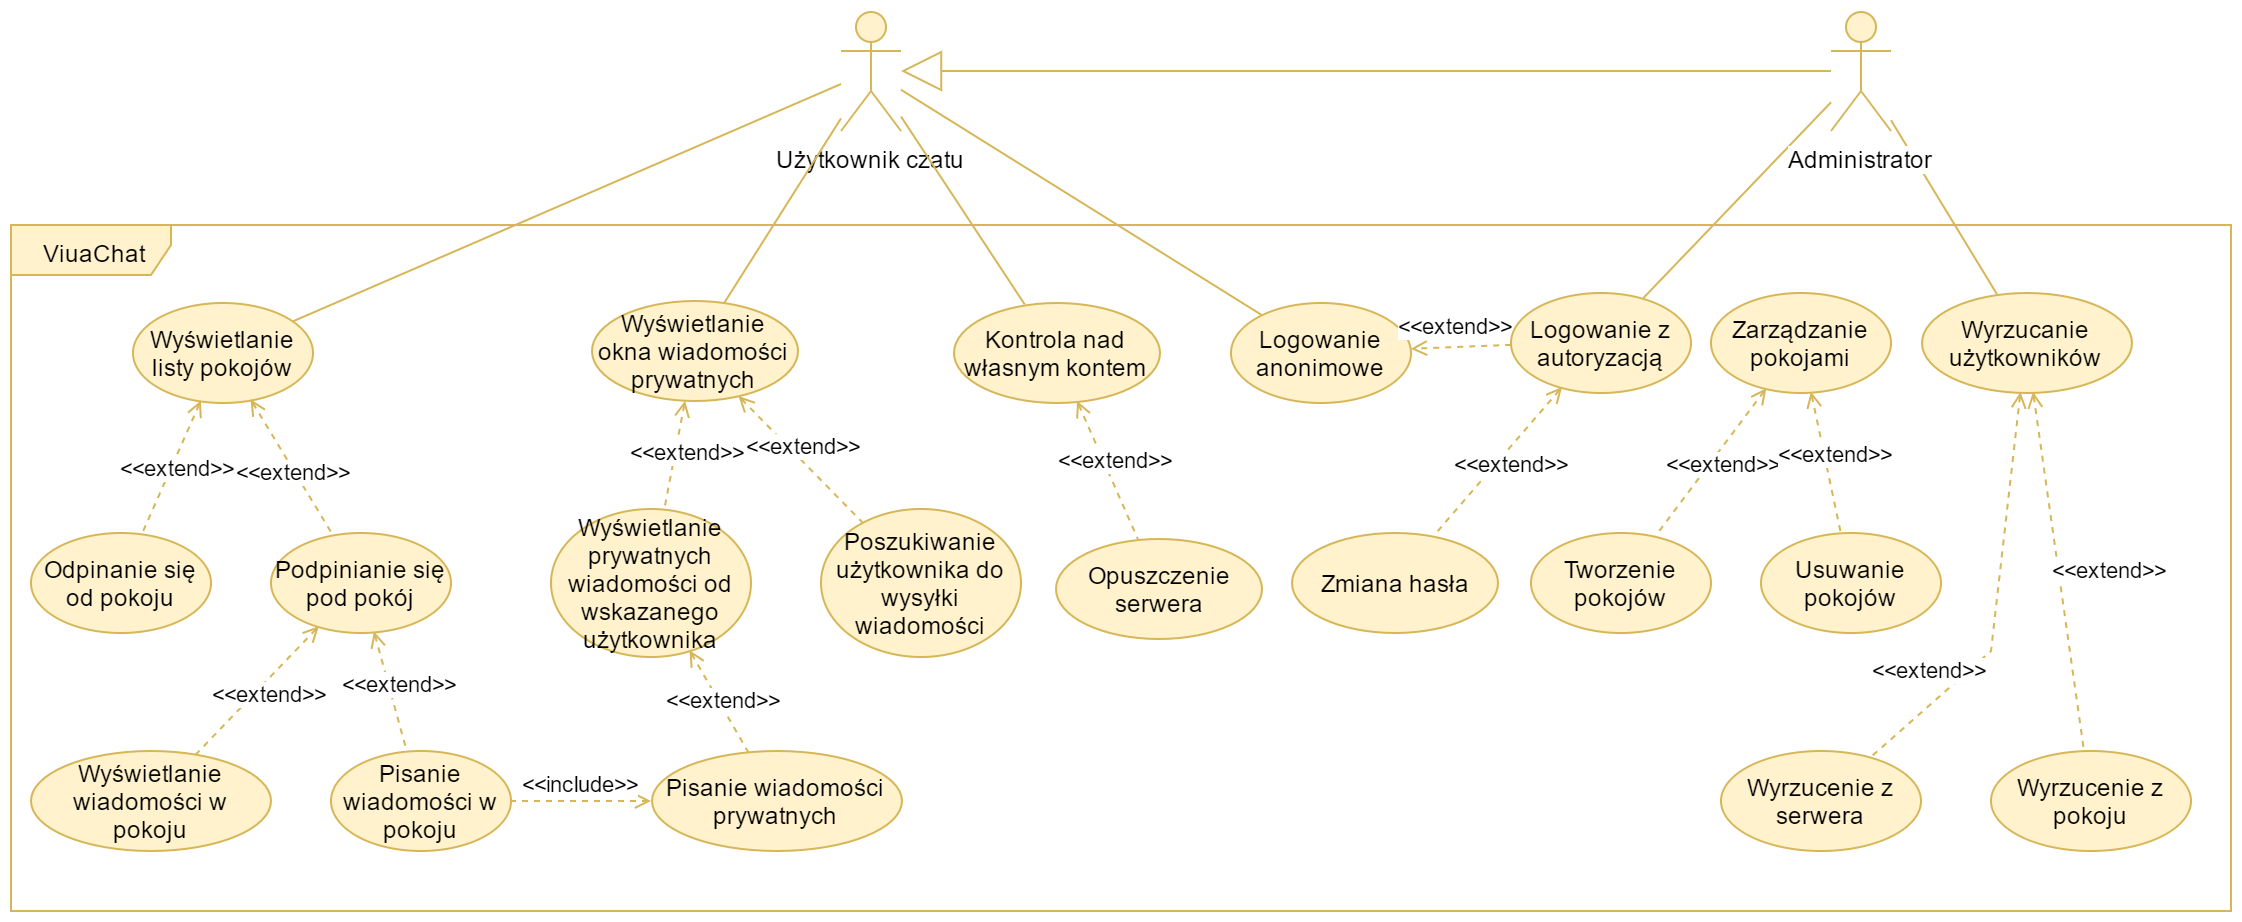
\includegraphics[width=\textwidth]{chat/fig/dpu-chat-v2}
	\caption{Diagram przypadków użycia aplikacji ViuaChat}
	\label{dpu-chat-v2}
\end{figure}

\subsection{Opis aktorów}

\textit{Uwaga! W niniejszej sekcji, słowo ,,aktor'' jest używane w rozumieniu
języka UML, a nie języka \ViuAct.}

\begin{enumerate}
	\item \textbf{Użytkownik czatu.} Typ użytkownika, którego konto
	jest tworzone podczas połączenia z serwerem czatu oraz niszczone po jego
	zakończeniu. Podczas łączenia z czatem, nie będzie musiał się autoryzować przy
	użyciu hasła, a deklarować tylko unikalną nazwę, nie powtarzającą się z nazwą
	innego użytkownika, posiadającego konto na danym serwerze czatu. Ten typ konta
	jest przeznaczony dla osób, zainteresowanych dołączeniem do dyskusji na czacie
	bez dodatkowych zobowiązań. Jest aktorem aktywnym i głównym.

	\item \textbf{Administrator.} To użytkownik, który jest dodatkowo
	wyróżniony i posiada uprawienia do szeroko pojętego zarządzania serwerem (w
	tym - pozostałymi użytkownikami). Konto administratora jest
	utrzymywane przez serwer pomiędzy połączeniami do czatu. Każdorazowo, przed
	rozpoczęciem sesji połączenia z serwerem, administratorzy muszą się dodatkowo
	autoryzować przyużyciu hasła. Równocześnie, ich nazwa jest zarezerwowana
	wyłącznie do jego	użytku oraz niedostępna	dla użytkowników tymczasowych. Nie
	wyróżnia się wśród administratorów żadnych dodatkowych, szczególnych ról
	(np. superadministrator, właściciel). Jest aktorem aktywnym i głównym.

\end{enumerate}

\subsection{Opis przypadków użycia}

Poniżej opisano przypadki użycia ujęte na rysunku \ref{dpu-chat-v2}
\nameref{dpu-chat-v2}.

{\footnotesize

\vspace{2em}

\begin{tabularx}{\textwidth}{|l|X|}
	\hline
		\textbf{Identyfikator} &
		UC-01
		\\

	\hline
		\textbf{Nazwa} &
		Logowanie anonimowe
		\\

	\hline
		\textbf{Aktorzy} &
			Użytkownik czatu
		\\

	\hline
		\textbf{Streszczenie} &
			Użytkownik rozpoczyna korzystanie z czatu pod wybraną nazwą
			użytkownika, ale bez konieczności podawania hasła.
		\\

	\hline
		\textbf{Warunek wstępny} &
			Użytkownik nie ma rozpoczętej sesji połączenia z serwerem
		\\

	\hline
		\textbf{Wyjątki} &
			\begin{itemize}
				\item Użytkownik ma już wcześniej rozpoczętą sesję z serwerem
			\end{itemize}
		\\

	\hline
		\textbf{Scenariusz podstawowy} &
			\begin{enumreq}
				\item Użytkownik wprowadza nazwę użytkownika i zatwierdza
				\item System sprawdza czy nazwa użytkownika jest wolna
				\item Gdy nazwa jest wolna, serwer rozpoczyna sesję	z użytkownikiem
			\end{enumreq}
		\\

	\hline
		\textbf{Scenariusze alternatywne} &
			\begin{enumreq}
				\item Gdy nazwa użytkownika jest zajęta (przez zalogowanego
				użytkownika lub stałe konto użytkownika), logowanie nie
				powiedzie się.
			\end{enumreq}
		\\

	\hline
		\textbf{Warunek końcowy} &
			Użytkownik ma rozpoczętą sesję z serwerem.
		\\

	\hline
		\textbf{Komentarz} &
			\textit{Brak}
		\\

	\hline
\end{tabularx}

\vspace{2em}

\begin{tabularx}{\textwidth}{|l|X|}
	\hline
		\textbf{Identyfikator} &
		UC-02
		\\

	\hline
		\textbf{Nazwa} &
		Logowanie z autoryzacją
		\\

	\hline
		\textbf{Aktorzy} &
			Administrator
		\\

	\hline
		\textbf{Streszczenie} &
			Administrator rozpoczyna korzystanie z czatu z wykorzystaniem stałego
			konta użytkownika. Podczas logowania, administrator, oprócz podana samej
			nazwy użytkownika, dodatkowo uwierzytelnia się hasłem, aby zweryfikować
			czy ma prawo do wykorzystywania konta.
		\\

	\hline
		\textbf{Warunek wstępny} &
			\begin{enumerate}
				\item Użytkownik nie ma rozpoczętej żadnej sesji połączenia z serwerem.
				\item Użytkownik posiadał wcześniej skonfigurowane konto administratora
				na serwerze
			\end{enumerate}
		\\

	\hline
		\textbf{Wyjątki} &
			\begin{itemize}
				\item Użytkownik ma już wcześniej rozpoczętą sesję z serwerem
			\end{itemize}
		\\

	\hline
		\textbf{Scenariusz podstawowy} &
			\begin{enumerate}
				\item Użytkownik wprowadza nazwę użytkownika, hasło	i zatwierdza
				\item Gdy istnieje konto administratora o wskazanej nazwie, a podane
				hasło jest z nim zgodne, wówczas serwer rozpoczyna sesję z
				użytkownikiem.
			\end{enumerate}
		\\

	\hline
		\textbf{Scenariusze alternatywne} &
			\begin{enumerate}
				\item Gdy nie istnieje konto administratora o podanej nazwie,
				próba zalogowania z hasłem nie powiedzie się - w przypadku logowania bez
				użycia hasła, patrz UC-01.
				\item Gdy podane hasło nie jest zgodne z hasłem do konta administratora
				o podanej nazwie, logowanie nie powiedzie	się.
			\end{enumerate}
		\\

	\hline
		\textbf{Warunek końcowy} &
			Użytkownik ma rozpoczętą sesję z serwerem.
		\\

	\hline
		\textbf{Komentarz} &
			\textit{Brak}
		\\

	\hline
\end{tabularx}

\vspace{2em}

\begin{tabularx}{\textwidth}{|l|X|}
	\hline
		\textbf{Identyfikator} &
		UC-03
		\\

	\hline
		\textbf{Nazwa} &
		Wyświetlanie listy pokojów
		\\

	\hline
		\textbf{Aktorzy} &
			Użytkownik czatu
		\\

	\hline
		\textbf{Streszczenie} &
			Użytkownik uzyskuje wgląd do listy pokojów z której może wybrać ten, do
			którego chce się podpiąć.
		\\

	\hline
		\textbf{Warunek wstępny} &
			\begin{enumreq}
				\item Użytkownik ma rozpoczętą sesję z serwerem
			\end{enumreq}
		\\

	\hline
		\textbf{Wyjątki} &
			\begin{enumreq}
				\item Użytkownik nie może być wcześniej podpięty do żadnego pokoju.
			\end{enumreq}
			\textit{Brak}
		\\

	\hline
		\textbf{Scenariusz podstawowy} &
			\begin{enumreq}
				\item Użytkownik wybiera z górnego menu opcję ,,Pokoje''.
				\item Pokazywany jest ekran listy pokojów.
				\item Użytkownik wybiera z listy nazwę pokoju, do którego chce
				się wpiąć.
			\end{enumreq}
		\\

	\hline
		\textbf{Scenariusze alternatywne} &
			\begin{enumreq}
				\item Wiadomości prywatne są wysyłane z okna czatu w
				specyficzny sposób (patrz UC-10)
				\item Tuż po zalogowaniu do serwera, scenariusz podstawowy zaczyna się
				od kroku 2.
			\end{enumreq}
		\\

	\hline
		\textbf{Warunek końcowy} &
			Użytkownik wybrał pokój do wpięcia się.
		\\

	\hline
		\textbf{Komentarz} &
			\textit{Brak}
		\\

	\hline
\end{tabularx}

\vspace{2em}

\begin{tabular}{ | l | l | }
	\hline
		\textbf{Identyfikator} &
		UC-04
		\\

	\hline
		\textbf{Nazwa} &
		Podpinanie się pod pokój
		\\

	\hline
		\textbf{Aktorzy} & \parbox[t]{11cm}{
			Użytkownik czatu
		}\\

	\hline
		\textbf{Streszczenie} & \parbox[t]{11cm}{
			Użytkownik czatu, po wybraniu pokoju z listy pokojów, jest
			do niego wpinany.

		}\\

	\hline
		\textbf{Warunek wstępny} & \parbox[t]{11cm}{
			\begin{enumreq}
				\item Użytkownik wybrał pokój z listy pokojów.
			\end{enumreq}

		}
		\\

	\hline
		\textbf{Wyjątki} & \parbox[t]{11cm}{
			\begin{enumreq}
				\item Użytkownik nie może być wcześniej wpięty do żadnego pokoju.
			\end{enumreq}

		}
		\\

	\hline
		\textbf{Scenariusz podstawowy} & \parbox[t]{11cm}{
			\begin{enumreq}
				\item Użytkownik wybiera pokój z listy
				\item Serwer weryfikuje, czy użytkownik nie był już wcześniej wpięty do
				innego pokoju
				\item Jeżeli użytkownik pozostawał wcześniej niepodpięty, serwer
				sprawdza, czy wybrany pokój nadal istnieje,
				\item Jeżeli pokój nadal istnieje, następuje podpięcie użytkownika pod
				wybrany pokój.
				\item Uzytkownikowi, który zostaje nowo podpięty do pokoju,	pokazywane
				jest 10 wiadomości wysłanych tuż przed jego dołączeniem do tego pokoju.
			\end{enumreq}
		}
		\\

	\hline
		\textbf{Scenariusze alternatywne} & \parbox[t]
		{11cm}{
			\begin{enumreq}
				\item Gdy użytkownik był wcześniej wpięty do innego pokoju,	najpierw
				zostaje od niego odpięty (UC-05), a dopiero później zostaje wpięty do
				wybranego pokoju.
			\end{enumreq}
		}
		\\

	\hline
		\textbf{Warunek końcowy} & \parbox[t]{11cm}{
			Użytkownik został podpięty pod pokój.
		}
		\\

	\hline
		\textbf{Komentarz} & \parbox[t]{11cm}{
			\textit{Brak}
		}
		\\

	\hline
\end{tabular}

\vspace{2em}

\begin{tabular}{ | l | l | }
	\hline
		\textbf{Identyfikator} &
		UC-05
		\\

	\hline
		\textbf{Nazwa} &
		Odpinanie się od pokoju
		\\

	\hline
		\textbf{Aktorzy} & \parbox[t]{11cm}{
			Użytkownik czatu
		}\\

	\hline
		\textbf{Streszczenie} & \parbox[t]{11cm}{
			Użytkownik, który był wcześniej wpięty do pokoju, może się od niego
			odpiąć, aby wpiąć się do innego pokoju lub po prostu zrezygnować z dalszej
			konwersacji.
		}\\

	\hline
		\textbf{Warunek wstępny} & \parbox[t]{11cm}{
			\begin{enumreq}
				\item Użytkownik ma rozpoczętą sesję z serwerem
				\item Użytkownik jest podpięty do pokoju
			\end{enumreq}

		}
		\\

	\hline
		\textbf{Wyjątki} & \parbox[t]{11cm}{
			\textit{Brak}
		}
		\\

	\hline
		\textbf{Scenariusz podstawowy} & \parbox[t]{11cm}{
			\begin{enumreq}
				\item Użytkownik wybiera przycisk ,,Opuść pokój''.
				\item Serwer weryfikuje, czy użytkownik nadal jest podpięty pod pokój.
				\item Jeżeli użytkownik jest nadal podpięty, następuje odpięcie.
				\item Użytkownik zostaje przekierowany do listy pokojów (UC-03 od kroku
				2)
			\end{enumreq}
		}
		\\

	\hline
		\textbf{Scenariusze alternatywne} & \parbox[t]
		{11cm}{
			\begin{enumreq}
				\item Gdy użytkownik pozostawał wcześniej niepodpięty, akcja kończy się
				niepowodzeniem.
			\end{enumreq}
		}
		\\

	\hline
		\textbf{Warunek końcowy} & \parbox[t]{11cm}{
			Użytkownik zostaje odpięty od pokoju.
		}
		\\

	\hline
		\textbf{Komentarz} & \parbox[t]{11cm}{
			\textit{Brak}
		}
		\\

	\hline
\end{tabular}

\vspace{2em}

\begin{tabular}{ | l | l | }
	\hline
		\textbf{Identyfikator} &
		UC-06
		\\

	\hline
		\textbf{Nazwa} &
		Pisanie wiadomości w pokoju
		\\

	\hline
		\textbf{Aktorzy} & \parbox[t]{11cm}{
			Użytkownik czatu
		}\\

	\hline
		\textbf{Streszczenie} & \parbox[t]{11cm}{
			Użytkownik może napisać wiadomość w pokoju czatu, którą zobaczą
			inni użytkownicy podpięci do tego pokoju (włącznie z jej nadawcą)
		}\\

	\hline
		\textbf{Warunek wstępny} & \parbox[t]{11cm}{
			\begin{enumreq}
				\item Użytkownik ma rozpoczętą sesję z serwerem
				\item Użytkownik jest podpięty do pokoju
			\end{enumreq}

		}
		\\

	\hline
		\textbf{Wyjątki} & \parbox[t]{11cm}{
			\textit{Brak}
		}
		\\

	\hline
		\textbf{Scenariusz podstawowy} & \parbox[t]{11cm}{
			\begin{enumreq}
				\item Użytkownik pisze wiadomość w polu tekstowym pod wiadomościami
				czatu.
				\item Po zatwierdzeniu wiadomości do wysyłki, pole tekstowe jest
				czyszczone.
				\item Gdy użytkownik jest nadal podpięty do pokoju, wiadomość zostaje
				wpisana do listy wiadomości i rozesłana do wszystkich	użytkowników.
				\item Użytkownik widzi swoją wiadomość wyświetloną u dołu ekranu.
			\end{enumreq}
		}
		\\

	\hline
		\textbf{Scenariusze alternatywne} & \parbox[t]
		{11cm}{
			\begin{enumreq}
				\item Gdy użytkownik nie był wpięty do pokoju w momencie wysyłania
				wiadomości, wysyłka kończy się niepowodzeniem
				\item Gdy wiadomość jest poprzedzona znakiem ..\#'', to jest realizowany
				scenariusz UC-11
			\end{enumreq}
		}
		\\

	\hline
		\textbf{Warunek końcowy} & \parbox[t]{11cm}{
			Wiadomość została zaakceptowania do rozesłania przez serwer.
		}
		\\

	\hline
		\textbf{Komentarz} & \parbox[t]{11cm}{
			\textit{Brak}
		}
		\\

	\hline
\end{tabular}

\vspace{2em}

\begin{tabular}{ | l | l | }
	\hline
		\textbf{Identyfikator} &
		UC-08
		\\

	\hline
		\textbf{Nazwa} &
		Wyświetlanie wiadomości prywatnych w pokoju
		\\

	\hline
		\textbf{Aktorzy} & \parbox[t]{11cm}{
			Użytkownik czatu
		}\\

	\hline
		\textbf{Streszczenie} & \parbox[t]{11cm}{
			Użytkownik widzi wiadomości prywatne, skierowane do niego przez
			innego użytkownika podpiętego do tego samego pokoju. Wiadomości
			tych nie widzi żaden inny użytkownik podpięty do pokoju, oprócz
			jej nadawcy i odbiorcy.

		}\\

	\hline
		\textbf{Warunek wstępny} & \parbox[t]{11cm}{
			\begin{enumreq}
				\item Użytkownik ma rozpoczętą sesję z serwerem
				\item Użytkownik jest podpięty do pokoju
				\item Użytkownik wysłał wiadomość do pokoju (patrz UC-07)
				poprzedzoną znakiem ,,\#''
			\end{enumreq}

		}
		\\

	\hline
		\textbf{Wyjątki} & \parbox[t]{11cm}{
			\textit{Brak}

		}
		\\

	\hline
		\textbf{Scenariusz podstawowy} & \parbox[t]{11cm}{
			\begin{enumreq}
				\item Użytkownik wysyła do pokoju wiadomość poprzedzoną znakiem ,,\#''.
				\item Serwer sprawdza, czy przed treścią wiadomości znajduje się łańcuch
				znaków będący prawidłową nazwą użytkownika.
				\item Jeżeli forma nazwy jest prawidłowa, serwer sprawdza, czy
				użytkownik wskazany na początku wiadomości jest podpięty do pokoju.
				\item Jeżeli użytkownik jest podpięty do pokoju, wiadomość zostaje
				przyjęta przez serwer jako wiadomość prywatna.
			\end{enumreq}
		}
		\\

	\hline
		\textbf{Scenariusze alternatywne} & \parbox[t]
		{11cm}{
			\begin{enumreq}
				\item Gdy nazwa użytkownika odbiorcy ma nieprawidłową formę, wiadomość
				nie zostanie przyjęta przez serwer i wysyłka zakończy się niepowodzeniem
				\item Gdy odbiorca wiadomości nie jest podpięty pod pokój, wiadomość nie
				zostanie przyjęta przez serwer i wysyłka zakończy się niepowodzeniem.
			\end{enumreq}
		}
		\\

	\hline
		\textbf{Warunek końcowy} & \parbox[t]{11cm}{
			Wiadomość prywatna została przyjęta przez serwer.
		}
		\\

	\hline
		\textbf{Komentarz} & \parbox[t]{11cm}{
			\textit{Brak}
		}
		\\

	\hline
\end{tabular}

\vspace{2em}

\begin{tabular}{ | l | l | }
	\hline
		\textbf{Identyfikator} &
		UC-09
		\\

	\hline
		\textbf{Nazwa} &
		Wyświetlanie okna wiadomości prywatnych
		\\

	\hline
		\textbf{Aktorzy} & \parbox[t]{11cm}{
			Użytkownik czatu
		}\\

	\hline
		\textbf{Streszczenie} & \parbox[t]{11cm}{
			Użytkownik może zobaczyć okno z wiadomościami prywatnymi (niezależnie od
			tego czy zostały wysłane z pokoju czy z okna wiadomości prywatnych),
			pogrupowane wg ich nadawców/odbiorców
		}\\

	\hline
		\textbf{Warunek wstępny} & \parbox[t]{11cm}{
			\begin{enumreq}
				\item Użytkownik ma rozpoczętą sesję z serwerem.
			\end{enumreq}

		}
		\\

	\hline
		\textbf{Wyjątki} & \parbox[t]{11cm}{
			\textit{Brak}

		}
		\\

	\hline
		\textbf{Scenariusz podstawowy} & \parbox[t]{11cm}{
			\begin{enumreq}
				\item Użytkownik wybiera z menu opcję ,,PW''
				\item Użytkownikowi zostaje pokazana lista nazw użytkowników,	od których
				otrzymał lub którym wysyłał wiadomości prywatne.
			\end{enumreq}
		}
		\\

	\hline
		\textbf{Scenariusze alternatywne} & \parbox[t]
		{11cm}{
			\begin{enumreq}
				\item Gdy użytkownik nie wysłał ani nie odebrał żadnych wiadomości
				prywatnych, lista nazw użytkowników będzie pusta.
			\end{enumreq}
		}
		\\

	\hline
		\textbf{Warunek końcowy} & \parbox[t]{11cm}{
			Użytkownik zobaczy listę nazw użytkowników, od których otrzymał lub którym
			wysłał wiadomości prywatne.
		}
		\\

	\hline
		\textbf{Komentarz} & \parbox[t]{11cm}{
			\textit{Brak}
		}
		\\

	\hline
\end{tabular}

\vspace{2em}

\begin{tabular}{ | l | l | }
	\hline
		\textbf{Identyfikator} &
		UC-10
		\\

	\hline
		\textbf{Nazwa} &
		Wyświetlanie prywatnych wiadomości od wskazanego użytkownika
		\\

	\hline
		\textbf{Aktorzy} & \parbox[t]{11cm}{
			Użytkownik czatu
		}\\

	\hline
		\textbf{Streszczenie} & \parbox[t]{11cm}{
			Użytkownik musi wybrać konkretnego innego użytkownika, aby zobaczyć jego
			wiadomości (tj. wiadomości prywatne, których jest nadawcą/odbiorcą).

		}\\

	\hline
		\textbf{Warunek wstępny} & \parbox[t]{11cm}{
			\begin{enumreq}
				\item Użytkownik wybrał nazwę użytkownika w oknie wiadomości prywatnych.
			\end{enumreq}

		}
		\\

	\hline
		\textbf{Wyjątki} & \parbox[t]{11cm}{
		\begin{enumreq}
		 \item Użytkownik nie wysłał ani nie odebrał dotychczas żadnych wiadomości
		 prywatnych.
	 	\end{enumreq}

		}
		\\

	\hline
		\textbf{Scenariusz podstawowy} & \parbox[t]{11cm}{
			\begin{enumreq}
				\item Użytkownik wybiera jedną z nazw, którą widzi na liście w oknie
				wiadomości prywatnych
				\item Użytkownikowi pokazywana jest lista wiadomości prywatnych, które
				otrzymał od tego użytkownika lub do których je skierował.
			\end{enumreq}
		}
		\\

	\hline
		\textbf{Scenariusze alternatywne} & \parbox[t]
		{11cm}{
			\begin{enumreq}
				\item Gdy wybrany użytkownik nie istnieje i/lub nie jest połączony z
				serwerem, operacja zakończy się błędem.
			\end{enumreq}
		}
		\\

	\hline
		\textbf{Warunek końcowy} & \parbox[t]{11cm}{
			Użytkownik zobaczył wiadomości prywatne, które odebrał od lub nadał do
			konkretnego użytkownika.
		}
		\\

	\hline
		\textbf{Komentarz} & \parbox[t]{11cm}{
			\textit{Brak}
		}
		\\

	\hline
\end{tabular}

\vspace{2em}

\begin{tabular}{ | l | l | }
	\hline
		\textbf{Identyfikator} &
		UC-11
		\\

	\hline
		\textbf{Nazwa} &
		Pisanie prywatnych wiadomości
		\\

	\hline
		\textbf{Aktorzy} & \parbox[t]{11cm}{
			Użytkownik czatu
		}\\

	\hline
		\textbf{Streszczenie} & \parbox[t]{11cm}{
			Użytkownik w oknie wiadomości prywatnych pisze wiadomości, które są
			domyślnie uznawane za wiadomości prywatne skierowane do użytkownika, który
			został wcześniej wybrany.
		}\\

	\hline
		\textbf{Warunek wstępny} & \parbox[t]{11cm}{
			\begin{enumreq}
				\item Użytkownik jest w oknie wiadomości prywatnych.
				\item Użytkownik wybrał, czyje wiadomości ogląda (patrz UC-10)
			\end{enumreq}

		}
		\\

	\hline
		\textbf{Wyjątki} & \parbox[t]{11cm}{
			\begin{enumreq}
				\item Użytkownik wybrany w oknie czatu rozłączył się z serwerem, zanim
				wiadomość została wysłana.
			\end{enumreq}
		}
		\\

	\hline
		\textbf{Scenariusz podstawowy} & \parbox[t]{11cm}{
			\begin{enumreq}
				\item Użytkownik wpisuje wiadomość do pola tekstowego pod wiadomościami
				w oknie wiadomości prywatnych
				\item Użytkownik decyduje o wysłaniu wiadomości.
				\item Pole tekstowe zostaje wyczyszczone.
				\item Serwer przyjmuje wiadomość jako wiadomość prywatną i rozsyła do
				nadawcy i odbiorcy
				\item Użytkownik widzi wysłaną wiadomość u dołu pola tekstowego.
			\end{enumreq}
		}
		\\

	\hline
		\textbf{Scenariusze alternatywne} & \parbox[t]
		{11cm}{
			\begin{enumreq}
				\item Gdy wybrany użytkownik odłączył się od serwera, wysłanie
				wiadomości kończy się niepowodzeniem.
			\end{enumreq}
		}
		\\

	\hline
		\textbf{Warunek końcowy} & \parbox[t]{11cm}{
			Wiadomość została pokazana nadawcy i odbiorcy.
		}
		\\

	\hline
		\textbf{Komentarz} & \parbox[t]{11cm}{
			Wiadomości wysyłane z okna wiadomości prywatych nie muszą być
			poprzedzane znakiem ,,\#'' i nazwą odbiorcy. Użytkownik docelowy
			jest wnioskowany z tego, czyje wiadomości są obecnie pokazywane w
			oknie wiadomości prywatnych (patrz UC-10)
		}
		\\

	\hline
\end{tabular}

\vspace{2em}

\begin{tabular}{ | l | l | }
	\hline
		\textbf{Identyfikator} &
		UC-12
		\\

	\hline
		\textbf{Nazwa} &
		Wyrzucanie użytkowników z serwera
		\\

	\hline
		\textbf{Aktorzy} & \parbox[t]{11cm}{
			Administrator
		}\\

	\hline
		\textbf{Streszczenie} & \parbox[t]{11cm}{
			Administrator ma prawo w dowolnym momencie przerwać połączenie dowolnego
			użytkownika z serwerem.

		}\\

	\hline
		\textbf{Warunek wstępny} & \parbox[t]{11cm}{
			\begin{enumreq}
				\item Administrator ma rozpoczętą sesję z serwerem.
				\item Wybrany uzytkownik ma rozpoczetą sesję z serwerem i nadal jest z
				nim połączony.
			\end{enumreq}

		}
		\\

	\hline
		\textbf{Wyjątki} & \parbox[t]{11cm}{
			Nie jest możliwe wyrzucenie samego siebie.
		}
		\\

	\hline
		\textbf{Scenariusz podstawowy} & \parbox[t]{11cm}{
			\begin{enumreq}
				\item Administrator klika nazwę użytkownika (niezależnie od miejsca, w
				którym została wyświetlona).
				\item Z menu, administrator wybiera opcję ,,Wyrzuć z serwera''.
				\item Wskazany użytkownik zostaje niezwłocznie odpięty z pokoju (o ile
				był podpięty do któregokolwiek).
				\item Połączenie wybranego użytkownika zostaje zakończone.
			\end{enumreq}
		}
		\\

	\hline
		\textbf{Scenariusze alternatywne} & \parbox[t]
		{11cm}{
			\begin{enumreq}
				\item Gdy wybrany użytkownik nie jest już połączony z serwerem, akcja
				kończy się niepowodzeniem.
			\end{enumreq}
		}
		\\

	\hline
		\textbf{Warunek końcowy} & \parbox[t]{11cm}{
			Wskazany użytkownik został odłączony od serwera.
		}
		\\

	\hline
		\textbf{Komentarz} & \parbox[t]{11cm}{
			\textit{Brak}
		}
		\\

	\hline
\end{tabular}

\vspace{2em}

\begin{tabular}{ | l | l | }
	\hline
		\textbf{Identyfikator} &
		UC-13
		\\

	\hline
		\textbf{Nazwa} &
		Wyrzucanie użytkowników z pokojów
		\\

	\hline
		\textbf{Aktorzy} & \parbox[t]{11cm}{
			Administrator
		}\\

	\hline
		\textbf{Streszczenie} & \parbox[t]{11cm}{
			Administrator może odpiąć wybranego użytkownika od pokoju, do którego jest
			obecnie wpięty.
		}\\

	\hline
		\textbf{Warunek wstępny} & \parbox[t]{11cm}{
			\begin{enumreq}
				\item Administrator ma rozpoczętą sesję z serwerem.
				\item Wybrany użytkownik jest wpięty do jakiegokolwiek pokoju.
			\end{enumreq}
		}
		\\

	\hline
		\textbf{Wyjątki} & \parbox[t]{11cm}{
			\textit{Brak}

		}
		\\

	\hline
		\textbf{Scenariusz podstawowy} & \parbox[t]{11cm}{
			\begin{enumreq}
				\item Administrator klika nazwę użytkownika, przebywając w oknie pokoju.
				\item Z menu, administrator wybiera opcję ,,Wyrzuć z pokoju''.
				\item Wskazany użytkownik zostaje niezwłocznie odpięty z pokoju.
			\end{enumreq}
		}
		\\

	\hline
		\textbf{Scenariusze alternatywne} & \parbox[t]
		{11cm}{
			\begin{enumreq}
				\item Gdy użytkownik, przed podjęciem przez administratora decyzji o
				wyrzuceniu, sam wypiął się z pokoju lub zerwał połączenie z serwerem,
				operacja kończy się niepowodzeniem.
			\end{enumreq}
		}
		\\

	\hline
		\textbf{Warunek końcowy} & \parbox[t]{11cm}{
			Użytkownik został wypięty z pokoju.
		}
		\\

	\hline
		\textbf{Komentarz} & \parbox[t]{11cm}{
			\textit{Brak}
		}
		\\

	\hline
\end{tabular}

\vspace{2em}

\begin{tabular}{ | l | l | }
	\hline
		\textbf{Identyfikator} &
		UC-14
		\\

	\hline
		\textbf{Nazwa} &
		Tworzenie pokojów
		\\

	\hline
		\textbf{Aktorzy} & \parbox[t]{11cm}{
			Administrator
		}\\

	\hline
		\textbf{Streszczenie} & \parbox[t]{11cm}{
			Administrator ma prawo tworzyć i usuwać pokoje

		}\\

	\hline
		\textbf{Warunek wstępny} & \parbox[t]{11cm}{
			\begin{enumreq}
				\item Administrator ma rozpoczętą sesję z serwerem
			\end{enumreq}

		}
		\\

	\hline
		\textbf{Wyjątki} & \parbox[t]{11cm}{
			\textit{Brak}

		}
		\\

	\hline
		\textbf{Scenariusz podstawowy} & \parbox[t]{11cm}{
			\begin{enumreq}
				\item Administrator wchodzi w listę pokojów
				\item Administrator klika w ikonę plusa obok nagłówka listy
				\item Pokazany zostaje okno utworzenia nowego pokoju
				\item W oknie utworzenia nowego pokoju, administrator wpisuje nazwę
				pokoju.
				\item Administrator zatwierdza utworzenie pokoju.
				\item Jeżeli nazwa pokoju jest prawidłowa pod względem wymagań
				biznesowych, tworzony jest nowy pokój.
			\end{enumreq}
		}
		\\

	\hline
		\textbf{Scenariusze alternatywne} & \parbox[t]
		{11cm}{
			\begin{enumreq}
				\item Gdy nazwa pokoju pokrywa się z istniejącym pokojem lub nie spełnia
				wymagań biznesowych, administrator jest poproszony o podanie takiej,
				która jest prawidłowa.
				\item Gdy administrator wyjdzie z okna utworzenia nowego pokoju bez
				jego zatwierdzenia, pokój nie zostaje dodany.
			\end{enumreq}
		}
		\\

	\hline
		\textbf{Warunek końcowy} & \parbox[t]{11cm}{
			Pokój został utworzony.
		}
		\\

	\hline
		\textbf{Komentarz} & \parbox[t]{11cm}{
			\textit{Brak}
		}
		\\

	\hline
\end{tabular}

\vspace{2em}

\begin{tabular}{ | l | l | }
	\hline
		\textbf{Identyfikator} &
		UC-15
		\\

	\hline
		\textbf{Nazwa} &
		Usuwanie pokojów.
		\\

	\hline
		\textbf{Aktorzy} & \parbox[t]{11cm}{
			Administrator
		}\\

	\hline
		\textbf{Streszczenie} & \parbox[t]{11cm}{
			Administrator ma prawo usuwać pokoje z serwera.

		}\\

	\hline
		\textbf{Warunek wstępny} & \parbox[t]{11cm}{
			\begin{enumreq}
				\item Administrator ma rozpoczętą sesję z serwerem
			\end{enumreq}

		}
		\\

	\hline
		\textbf{Wyjątki} & \parbox[t]{11cm}{
			\textit{Brak}

		}
		\\

	\hline
		\textbf{Scenariusz podstawowy} & \parbox[t]{11cm}{
			\begin{enumreq}
				\item Administrator przechodzi do listy pokojów.
				\item Administrator klika w ikonę trzech pionowych kropek obok nazwy
				wybranego pokoju.
				\item W rozwijanym menu zostaje pokazana opcja ,,Usuń''.
				\item Zostaje pokazany monit z prośbą o potwierdzenie decyzji, w którym
				zostaje obowiązkowo wymieniona nazwa pokoju.
				\item Po zatwierdzeniu decyzji, użytkownicy wpięci do usuwanego pokoju
				zostają usunięte, a następnie sam pokój zostaje usunięty.
			\end{enumreq}
		}
		\\

	\hline
		\textbf{Scenariusze alternatywne} & \parbox[t]
		{11cm}{
			\begin{enumreq}
				\item Gdy pokój przestahe istnieć pomiędzy wybraniem a potwierdzeniem
				usunięcia, operacja zostanie zakończona niepowodzeniem.
				\item Gdy administrator zrezygnuje z usunięcia pokoju na etapie okna
				potwierdzającego usunięcie, pokój pozostanie nieusunięty.
			\end{enumreq}
		}
		\\

	\hline
		\textbf{Warunek końcowy} & \parbox[t]{11cm}{
			Pokój zostaje usunięty.
		}
		\\

	\hline
		\textbf{Komentarz} & \parbox[t]{11cm}{
			\textit{Brak}
		}
		\\

	\hline
\end{tabular}
}


\chapter{Wpływ pracy na platformę Viua VM}

W tym rozdziale omówiony jest wpływ naszej pracy inżynierskiej na platformę Viua VM; zarówno na implementację
samej maszyny wirtualnej i dopracowanie jej mechanizmów (np. doprowadzenie systemu modułów do stanu
używalności), ale też na ,,ekosystem'' dookoła niej -- nowe moduły biblioteki standardowej i zewnętrzne.

\section{System modułów}

Viua VM musiała zostać wyposażona w system modułów. Wymagane było przeprojektowanie i ,,ucywilizowanie''
stanu, w którym system modułów Viua VM się znajdował przed rozpoczęciem prac nad projektem inżynierskim.

\section{Moduł do obsługi protokołu WebSocket}

Do wykonania czatu potrzebny był moduł do obsługi protokołu WebSocket.

\chapter{Wkład własny członków zespołu}
\label{wklad_wlasny_czlonkow_zespolu}

\section{Krzysztof Franek}

\section{Marek Marecki}

\section{Słownik pojęć}
\label{slownik_pojec}

W tym rozdziale prezentujemy słownik pojęć używanych w pracy, a których znaczenie może być niejednoznaczne lub
nieznane czytelnikowi.
Pojęcia są ułożone w kolejności alfabetycznej.

\subsection{Pojęcia ogólne}
\label{slownik_pojec_ogolnych}

\begin{labeling}{interakcje języka z platformą}
    \item [FFI] (ang. \emph{foreign function interface}) interfejs umożliwiający wywoływanie z jednego języka
        funkcji napisanych w innym języku
    \item [ViuAct] język wysokiego poziomu, oparty o modelu aktorów, kompilowany
        do języka asemblera Viua VM
    \item [Viua VM] maszyna wirtualna, umożliwiająca uruchamianie programów
        wykorzystujących współbieżność
    \item[interakcje języka z platformą] wykorzystanie zasobów sprzętowych, operacje I/O, oraz wszelkie
        efekty uboczne będące wynikiem działania programu
\end{labeling}

\subsection{Pojęcia związane z językiem i kompilatorem}
\label{slownik_pojec_jezyka}

\begin{labeling}{jednostka translacji}
    \item[biblioteka] zbiór modułów
    \item[\emph{compile-time}] ,,\emph{czas kompilacji}''; czas, w którym program jest kompilowany
    \item[jądro] podsystem Viua VM odpowiadający za uruchamianie programów (tzw. ''\emph{kernel}'')
    \item[jednostka translacji] w przypadku języka ViuAct jest to pojedynczy moduł
    \item[kompilator] program tłumaczący kod w jednym języku (zazwyczaj wysokiego poziomu) na kod o takim
        samym znaczeniu w innym języku (zazwyczaj niższego poziomu)
    \item[leksem] ciąg znaków odpowiadający wzorcowi określającemu możliwe wartości tokenu
    \item[linker] program łączący wiele modułów w plik wykonywalny
    \item[moc funkcji] (ang. \emph{arity}) ilość parametrów formalnych przyjmowanych przez funkcję (pojęcie
        zapożyczone z pojęcia mocy zbioru)
    \item [model aktorów] model przetwarzania współbieżnego, opierający się na
        podstawowych strukturach, nazywanych „aktorami”, posiadających swój
        własny prywatny stan i porozumiewających się pomiędzy sobą za pomocą
        komunikatów
    \item[moduł] w załeżności od kontekstu: \emph{1/} kod źródłowy modułu w języku ViuAct, lub \emph{2/} plik
        zawierający bytecode w formacie, który może zostać wykorzystany przez linker bądź jądro Viua VM do
        dołączenia
    \item[plik wykonywalny] plik zawierający bytecode w formacie, który może zostać wykonany przez jądro Viua
        VM
    \item[runtime] ,,\emph{środowisko uruchomieniowe}''; maszyna wirtualna bądź realna, na której
        wykonywany jest program
    \item[\emph{run-time}] ,,\emph{czas wykonywania}''; czas, w którym program jest wykonywany przez VM;
        przeciwieństwo \emph{compile-time}
    \item[token] abstrakcyjna reprezentacja konkretnego elementu leksykalnego, np. słowa kluczowego lub
        identyfikatora, składająca się z nazwy typu tokenu i leksemu, który dana instancja tokenu zawiera
    \item[wzorzec] wyrażenie regularne określające jaką formę mogą przyjąć leksemy danego typu tokenu
\end{labeling}

\subsection{Pojęcia związane z chatem}
\label{slownik_pojec_chatu}

\begin{labeling}{Wpięcie użytkownika w pokój}
    \item[Pokój] Współdzielony czat, do którego dostęp ma równocześnie wielu uczestników, widzących nawzajem
        wysyłane przez siebie wiadomości
    \item[Wiadomości prywatne] Wiadomości, które są wysyłane konkretnemu użytkownikowi i są widoczne wyłącznie
        dla nadawcy i odbiorcy takiej wiadomości
    \item[Wpięcie użytkownika w pokój] Rodzaj relacji, polegający na tym, że dany użytkownik ma możliwość
        nadawania i odbierania wiadomości w ramach określonego pokoju
\end{labeling}


\chapter{Bibliografia}

Książki. Internetowe materiały. Materiały wykładowe. Opracowania własne.

\end{document}
